%  template.tex for Biometrics papers
%
%  This file provides a template for Biometrics authors.  Use this
%  template as the starting point for creating your manuscript document.
%  See the file biomsample.tex for an example of a full-blown manuscript.

%  ALWAYS USE THE referee OPTION WITH PAPERS SUBMITTED TO BIOMETRICS!!!
%  You can see what your paper would look like typeset by removing
%  the referee option.  Because the typeset version will be in two
%  columns, however, some of your equations may be too long. DO NOT
%  use the \longequation option discussed in the user guide!!!  This option
%  is reserved ONLY for equations that are impossible to split across 
%  multiple lines; e.g., a very wide matrix.  Instead, type your equations 
%  so that they stay in one column and are split across several lines, 
%  as are almost all equations in the journal.  Use a recent version of the
%  journal as a guide. 
%  
\documentclass[useAMS,usenatbib,referee]{biom}
%\documentclass[useAMS,usenatbib]{biom}
\usepackage{graphicx}
\usepackage{amsmath,amsfonts}
\usepackage{xcolor}
%\usepackage{amssymb}
%documentclass[useAMS]{biom}
%
%  If your system does not have the AMS fonts version 2.0 installed, then
%  remove the useAMS option.
%
%  useAMS allows you to obtain upright Greek characters.
%  e.g. \umu, \upi etc.  See the section on "Upright Greek characters" in
%  this guide for further information.
%
%  If you are using AMS 2.0 fonts, bold math letters/symbols are available
%  at a larger range of sizes for NFSS release 1 and 2 (using \boldmath or
%  preferably \bmath).
% 
%  Other options are described in the user guide. Here are a few:
% 
%  -  If you use Patrick Daly's natbib  to cross-reference your 
%     bibliography entries, use the usenatbib option
%
%  -  If you use \includegraphics (graphicx package) for importing graphics
%     into your figures, use the usegraphicx option
% 
%  If you wish to typeset the paper in Times font (if you do not have the
%  PostScript Type 1 Computer Modern fonts you will need to do this to get
%  smoother fonts in a PDF file) then uncomment the next line
%  \usepackage{Times}

%%%%% PLACE YOUR OWN MACROS HERE %%%%%

\def\bSig\bmath{\Sigma}
\newcommand{\VS}{V\&S}
\newcommand{\tr}{\mbox{tr}}
\newcommand{\tcr}[1]{\textcolor{red}{#1}}
\newcommand{\tcb}[1]{\textcolor{blue}{#1}}
\newcommand{\tco}[1]{\textcolor{orange}{#1}}
%  The rotating package allows you to have tables displayed in landscape
%  mode.  The rotating package is NOT included in this distribution, but
%  can be obtained from the CTAN archive.  USE OF LANDSCAPE TABLES IS
%  STRONGLY DISCOURAGED -- create landscape tables only as a last resort if
%  you see no other way to display the information.  If you do this,
%  then you need the following command.

%\usepackage[figuresright]{rotating}

%%%%%%%%%%%%%%%%%%%%%%%%%%%%%%%%%%%%%%%%%%%%%%%%%%%%%%%%%%%%%%%%%%%%%

%  Here, place your title and author information.  Note that in 
%  use of the \author command, you create your own footnotes.  Follow
%  the examples below in creating your author and affiliation information.
%  Also consult a recent issue of the journal for examples of formatting.

\title{A Structured Framework for Bayesian Sequential Monitoring in Clinical Trials}

%  Here are examples of different configurations of author/affiliation
%  displays.  According to the Biometrics style, in some instances,
%  the convention is to have superscript *, **, etc footnotes to indicate 
%  which of multiple email addresses belong to which author.  In this case,
%  use the \email{ } command to produce the emails in the display.

%  In other cases, such as a single author or two authors from 
%  different institutions, there should be no footnoting.  Here, use
%  the \emailx{ } command instead. 

%  The examples below correspond to almost every possible configuration
%  of authors and may be used as a guide.  For other configurations, consult
%  a recent issue of the journal.

%  Single author -- USE \emailx{ } here so that no asterisk footnoting
%  for the email address will be produced.

%\author{John Author\emailx{email@address.edu} \\
%Department of Statistics, University of Warwick, Coventry CV4 7AL, U.K.}

%  Two authors from the same institution, with both emails -- use
%  \email{ } here to produce the asterisk footnoting for each email address

%\author{John Author$^{*}$\email{author@address.edu} and
%Kathy Authoress$^{**}$\email{email2@address.edu} \\
%Department of Statistics, University of Warwick, Coventry CV4 7AL, U.K.}

%  Exactly two authors from different institutions, with both emails  
%  USE \emailx{ } here so that no asterisk footnoting for the email address
%  is produced.

%\author
%{John Author\emailx{author@address.edu} \\
%Department of Statistics, University of Warwick, Coventry CV4 7AL, U.K. 
%\and
%Kathy Author\emailx{anotherauthor@address.edu} \\
%Department of Biostatistics, University of North Carolina at Chapel Hill, 
%Chapel Hill, North Carolina, U.S.A.}

%  Three or more authors from same institution with all emails displayed
%  and footnoted using asterisks -- use \email{ } 

%\author{John Author$^*$\email{author@address.edu}, 
%Jane Author$^{**}$\email{jane@address.edu}, and 
%Dick Author$^{***}$\email{dick@address.edu} \\
%Department of Statistics, University of Warwick, Coventry CV4 7AL, U.K}

%  Three or more authors from same institution with one corresponding email
%  displayed

%\author{John Author$^*$\email{author@address.edu}, 
%Jane Author, and Dick Author \\
%Department of Statistics, University of Warwick, Coventry CV4 7AL, U.K}

%  Three or more authors, with at least two different institutions,
%  more than one email displayed 

%\author{John Author$^{1,*}$\email{author@address.edu}, 
%Kathy Author$^{2,**}$\email{anotherauthor@address.edu}, and 
%Wilma Flinstone$^{3,***}$\email{wilma@bedrock.edu} \\
%$^{1}$Department of Statistics, University of Warwick, Coventry CV4 7AL, U.K \\
%$^{2}$Department of Biostatistics, University of North Carolina at 
%Chapel Hill, Chapel Hill, North Carolina, U.S.A. \\
%$^{3}$Department of Geology, University of Bedrock, Bedrock, Kansas, U.S.A.}

%  Three or more authors with at least two different institutions and only
%  one email displayed

\author{Evan Kwiatkowski$^{1,*}$\email{ekwiatkowski@unc.edu}, 
Eugenio Andraca-Carrera$^{2}$, Mat Soukup$^{2}$, and Matthew A. Psioda$^{1}$ \\
$^{1}$Department of Biostatistics, University of North Carolina, \\
McGavran-Greenberg Hall, CB\#7420, \\
Chapel Hill, North Carolina, USA\\
$^{2}$Division of Biometrics VII, Office of Biostatistics, \\
Center for Drug Evaluation and Research, US Food and Drug Administration, \\
Silver Spring, Maryland, USA}

\DeclareMathOperator*{\argmax}{arg\,max}
\DeclareMathOperator*{\argmin}{arg\,min}

\begin{document}

%  This will produce the submission and review information that appears
%  right after the reference section.  Of course, it will be unknown when
%  you submit your paper, so you can either leave this out or put in 
%  sample dates (these will have no effect on the fate of your paper in the
%  review process!)


%\date{{\it Received October} 2007. {\it Revised February} 2008.  {\it
%Accepted March} 2008.}
\date{}

%  These options will count the number of pages and provide volume
%  and date information in the upper left hand corner of the top of the 
%  first page as in published papers.  The \pagerange command will only
%  work if you place the command \label{firstpage} near the beginning
%  of the document and \label{lastpage} at the end of the document, as we
%  have done in this template.

%  Again, putting a volume number and date is for your own amusement and
%  has no bearing on what actually happens to your paper!  

\pagerange{\pageref{firstpage}--\pageref{lastpage}} 

%\volume{64}
\volume{}
%\pubyear{2008}
\pubyear{}
%\artmonth{December}
\artmonth{}

%  The \doi command is where the DOI for your paper would be placed should it
%  be published.  Again, if you make one up and stick it here, it means 
%  nothing!

%\doi{10.1111/j.1541-0420.2005.00454.x}
\doi{}

%  This label and the label ``lastpage'' are used by the \pagerange
%  command above to give the page range for the article.  You may have 
%  to process the document twice to get this to match up with what you 
%  expect.  When using the referee option, this will not count the pages
%  with tables and figures.  

\label{firstpage}

%  put the summary for your paper here

\begin{abstract}

We present a Bayesian framework for sequential monitoring that allows for use of external data, and that 
can be applied in a wide range of clinical trial applications. The basis for this framework is the 
idea that, in many cases, specification of priors used for sequential monitoring and the stopping criteria can be semi-algorithmic 
byproducts of the trial hypotheses and relevant external data, simplifying the process of prior elicitation. 
Monitoring priors are defined using the family of generalized normal distributions which comprise a flexible class of priors, naturally allowing one to construct a prior that is peaked or flat about the parameter values thought to be most likely. External data are incorporated into the monitoring process though mixing an 
a priori skeptical prior with an enthusiastic one using a weight that can be fixed or adaptively estimated based on the degree to which observed data are better supported by a skeptical perspective versus an enthusiastic one. 
%
The proposed method is applied in two examples: (1) a single-arm proof-of-concept trial and (2) a two-arm randomized 
controlled trial. Both examples are motivated by completed pediatric trials, and the designs incorporate information from adult 
trials to varying degrees. Preposterior analysis of each trial design is performed to illustrate that the proposed Bayesian 
approaches provide reasonable frequentist operating characteristics without having that explicit focus.

\end{abstract}

%  Please place your key words in alphabetical order, separated
%  by semicolons, with the first letter of the first word capitalized,
%  and a period at the end of the list.
%

\begin{keywords}
Adaptive Trial Design; Bayesian Sequential Monitoring; Information Borrowing; Pediatric Trials; Skeptical Prior
\end{keywords}

%  As usual, the \maketitle command creates the title and author/affiliations
%  display 

\maketitle

%  If you are using the referee option, a new page, numbered page 1, will
%  start after the summary and keywords.  The page numbers thus count the
%  number of pages of your manuscript in the preferred submission style.
%  Remember, ``Normally, regular papers exceeding 25 pages and Reader Reaction 
%  papers exceeding 12 pages in (the preferred style) will be returned to 
%  the authors without review. The page limit includes acknowledgements, 
%  references, and appendices, but not tables and figures. The page count does 
%  not include the title page and abstract. A maximum of six (6) tables or 
%  figures combined is often required.''

%  You may now place the substance of your manuscript here.  Please use
%  the \section, \subsection, etc commands as described in the user guide.
%  Please use \label and \ref commands to cross-reference sections, equations,
%  tables, figures, etc.
%
%  Please DO NOT attempt to reformat the style of equation numbering!
%  For that matter, please do not attempt to redefine anything!

\section{Introduction}

In the United States, sponsors of trials evaluating new drugs, biologics, and devices are required to monitor these trials \citep{FDA2006}. 
%
While monitoring of trials takes on various forms, one form of monitoring is to assess the safety and efficacy of a product in an ongoing trial at pre-defined intervals (i.e. interim analyses), typically through an independent data monitoring committee. 
%
The most commonly used statistical approach to account for interim analyses are frequentist group sequential methods in which Type I error for testing a null and alternative hypothesis is distributed across the set of interim analyses to ensure overall Type I error control for establishing the efficacy or futility of a product \citep{Jennison2000}.  
%
%Bayesian monitoring of sequential trials is an alternative to the frequentist approach. 
Alternatively, in Bayesian sequential monitoring data can be monitored on a continual basis and the evidence in favor (or against) a hypothesis can be evaluated against a single standard without penalty \citep{Spiegelhalter1993}. %
%Under this paradigm, data is monitored and collection stopped when any of the following conditions are met (a) a sufficiently skeptical person is convinced the alternative hypothesis is true (b) a sufficiently enthusiastic person is convinced the alternative is false or the benefit of treatment is not as high as expected (c) the probability of eventually proving the alternative is true is sufficiently low or (d) all resources allocated have been exhausted \citep{Spiegelhalter1993} .

In the clinical development of a therapeutic product, external forces may impede a clinical trial from reaching its objective (e.g. difficulty in enrolling, limited patient populations, long latency in observing the outcome of interest, etc.). 
%
This challenge is especially apparent in cases where the disease for which the investigational product (IP) is an intended treatment is rare or where the focus is on pediatric disease. 
%
In settings where patients are difficult to enroll, and therefore meaningful numbers of patients will complete follow up prior to the trial reaching full enrollment, the concept of frequently monitoring interim data to determine whether a trial (or enrollment) can be stopped becomes appealing. 
%
As such, the use of Bayesian sequential methods, rooted in the likelihood principle and thus completely consistent with frequent or even continual data monitoring, provide an ideal basis from which to develop Complex Innovative Designs (CIDS) – a performance goal set forth under PDUFA VI legislation \citep{FDA2017}.
%
Moreover, in settings where pertinent preexisting data are available, Bayesian methods provide a natural approach for incorporating that information via a prior distribution into the design and analysis of a future trial.
%
The potential use of Bayesian methods is discussed throughout the draft guidance \citep{FDA_CID}, created in response to the 21st Century Cures Act \citep{USCongress2016}, including the use of Bayesian methods to extrapolate information from adult patients to pediatric settings as one type of possible CID (see Section III, Part C).

%Enrolling the number of patients needed to adequately address objectives of a clinical trial can be difficult.
%% 
%This challenge is especially apparent in cases where the disease for which the investigational product (IP) is an 
%intended treatment is rare or where the focus is on pediatric disease.
%%
%There is increased interest in innovative ways to perform trials in these settings to facilitate obtaining substantial
%evidence of treatment benefit as efficiently as possible given the challenge of enrolling patients in a timely fashion.
%%
%Indeed, this is exemplified by the draft guidance from the United States Food and Drug Administration (FDA) which outlines
%procedures for interacting with FDA on complex innovative trial designs \citep{FDA_CID}, abbreviated CIDs, and the FDA CID Pilot 
%Program which was initiated to fulfill a performance goal set forth under the PDUFA IV legislation.
%%
%In the draft guidance (see Section II), CIDs are defined as ``trial designs that have rarely or never been used 
%to date to provide substantial evidence of effectiveness in new drug applications or biologics license applications.''
%%
%The potential use of Bayesian methods are discussed throughout the draft guidance and, in particular, the use of Bayesian methods
%to extrapolate information from adult patients to pediatric settings is given as one type of possible CID (see Section 
%II, Part C).
%
%In settings where patients are difficult to enroll, and therefore meaningful numbers of patients will complete follow up prior to 
%the trial reaching full enrollment, the concept of frequently monitoring interim data to determine whether a trial 
%(or enrollment) can be stopped becomes appealing. 
%%
%A promising interim analysis that provides substantial evidence of efficacy may justify ending enrollment, while enrolled patients may continue 
%to receive the treatment for the pre-planned period of exposure. 
%%
%A discouraging interim analysis that provides substantial evidence of futility may justify ending enrollment, and may call for enrolled patients 
%who are ongoing in the trial to be transitioned off the IP (i.e., termination of investigation of the treatment). 
%%
%For the Bayesian, the question becomes ``From what prior perspective must the evidence be substantial to justify one of the two actions described above?'' 
%%
%This motivates the notion of skeptical and enthusiastic perspectives.
%%
%The use of monitoring based on changing the opinion of skeptical and enthusiastic observers has been described as overcoming a 
%handicap \citep{Freedman1989} and providing a brake on the premature termination of trials \citep{Fayers1997}, and as 
%constructing ``an adversary who will need to be disillusioned by the data to stop further experimentation" \citep{Spiegelhalter1994}. 
%
%
%In the author's opinion, the use of Bayesian sequential methods, rooted in the likelihood principle and thus completely consistent with 
%frequent or even continual data monitoring, provide an ideal basis from which to develop CIDs 
%for these settings.
%%
%Moreover, in settings where pertinent preexisting data are available, Bayesian methods inarguably provide a natural 
%approach for incorporating that information via a prior distribution into the design and analysis of a future trial. 

In this paper, we propose a strategy for designing sequentially monitored clinical trials that entails eliciting 
priors used to monitor enrollment and/or data collection (i.e., monitoring priors) and stopping criteria that can 
be derived in a semi-automatic fashion based on standard inputs that are required for trial planning. 
%
These inputs include (1) the boundary null value for the treatment effect, (2) a plausible, clinically meaningful 
value for the treatment effect, and (3) a criteria for what constitutes a compelling demonstration of efficacy. 
%
In principle, the plausible, clinically meaningful value for the treatment effect should be informed by relevant external data, when available. 


A key contribution of this work is to give structured definitions for skeptical and enthusiastic perspectives that can be used 
to inform early stopping decisions in favor of efficacy and futility, respectively. Skeptical and enthusiastic priors are developed using the generalized normal family of distributions. 
	%
This flexible family includes the normal distribution as a special case, and provides the capacity to construct monitoring 
priors that reflect nuanced prior opinion about the treatment effect (Section \ref{sec:gen_normal}). 
	%
A conditional-marginal prior factorization is proposed for settings where there are one or more nuisance 
parameters (Section \ref{sec:cond_marg}) and we illustrate how prior information can be used in both marginal 
distribution for the treatment effect and conditional distribution for the nuisance parameters, if desired. 

We perform simulation-based preposterior analysis to examine a variety of operating characteristics for the proposed design framework,
and to understand how key operating characteristics are influenced by the frequency of monitoring.
%	%
%\textcolor{red}{General feedback: Compare this text against the previous version. There was a good deal of 
%confusing/inaccurate language -- e.g.,  coverage probability for the treatment effect or probability of early stopping
%at an interim or final analysis. We need all sentences to be 100\% conceptually and mathematically precise.}
	%
Specifically, we estimate the probability of stopping early at an interim analysis due to a compelling demonstration of efficacy or futility, the expected sample size and trial duration, the average posterior mean, and the coverage probabilities for 95\% credible intervals for the treatment effect. 
	%
In most cases, patients will be ongoing in the trial at the time interim data are obtained that lead to 
ending enrollment as a result of a compelling demonstration of efficacy. 
	%
It is our assumption that in most cases these patients will complete the study protocol and, accordingly, we also explore 
the degree that interim evidence changes on average, once final data are available.	

Bayesian sequential designs are often restricted to have explicit frequentist properties \citep{Ventz2015, Zhu2015}. 
	%
Prior work has shown such restrictions can result in Bayesian and frequentist designs that have stopping rules which are 
nearly identical \citep{Stallard2020, Kopp-Schneider2020, Zhu2019}.
	%
While it is possible to calibrate a Bayesian design to have specific frequentist operating characteristics, we do not advocate
for that strategy.
	%
Instead, we propose a Bayesian framework that leverages what the authors argue is an intuitive criteria for stopping enrollment 
and/or data collection at any point (based on posterior inference using a consistent criteria for a compelling demonstration) without 
explicit focus on strict type I error control -- something that is not achievable when prior information is incorporated into 
the analysis \citep{Psioda2018}.
	%
%\textcolor{green}{Please check the accuracy of the following claim.}
%As will be illustrated, when prior information is not incorporated into the analysis, the designs operating characteristics 
%are ``well-calibrated" as discussed by \cite{Grieve2016}. 

%\textcolor{green}{Please give a more granular breakdown of what is in the paper. In particular, please describe the content 
%in Section \ref{sec:methods} in more depth. You can go into what is in the subsections.}
This paper is organized as follows: %
Section \ref{sec:preliminaries} reviews Bayesian hypothesis testing using posterior probabilities and the use of  skeptical and enthusiastic priors for efficacy and futility monitoring. 
%
Section \ref{sec:mps} presents a method for parameterizing monitoring priors using the generalized normal distribution and for incorporating prior information into the monitoring priors, as well as construction of inference priors and a method to specify priors for nuisance parameters.
%
Examples are given in Section \ref{sec:examples}, with Section \ref{sec:example1} presenting an example based on a single-arm trial and Section \ref{sec:example2} presenting an example based on a two-arm randomized, controlled trial.
%Conclusions from Bayesian inferences are not affected by the frequency with which the data are monitored, and such interim analyses should be encouraged to terminate data collection if appropriate \citep{Berry1989,Berry1993,Spiegelhalter1994}. The Bayesian perspective is based on the likelihood principle which asserts that any data with the same likelihood function should lead to the same conclusion \citep{Berger1988}. In the context of sequential analysis of clinical trials, the stopping rule that leads to the termination of data collection is irrelevant to the conclusion \citep{Barnard1947,Anscombe1963,Cornfield1966a,Cornfield1966b}. 
%In contrast ... add stuff Frequentist group sequential designs rely on pre-specified interim analyses and spending functions to maintain desired trial operating characteristics \citep{Pocock1977,OBrien1979}.
%Interpretation of conclusions from the Bayesian perspective is natural when specification of prior distributions are intuitively related to the research objectives. Skeptical and enthusiastic monitoring priors are used to evaluate efficacy and futility at an interim analysis \citep{Freedman1989,Freedman1992,Spiegelhalter1993,Fayers1997}. The most common Bayesian metrics for assessing evidence at interim analyses are posterior probabilities and predictive probabilities, and the choice of metric depends on the research objective. Posterior probabilities assess the level of evidence in favor of the null or alternative hypothesis, and predictive probabilities determine the capacity for the trial to show convincing evidence in favor of the alternative hypothesis if more outcomes are ascertained. 
\section{Methods}\label{sec:methods}

\subsection{Preliminaries}\label{sec:preliminaries}
\subsubsection{Bayesian Hypothesis Testing}
Consider a clinical trial application where the primary objective is to test a hypothesis about an unknown quantity of interest which we denote by $\theta$, with possible values
for $\theta$ falling in the parameter space $\Theta$.
%
For example, in a single-arm trial with a binary response endpoint, $\theta \in (0,1)$ may be the response probability associated with patients receiving the IP.
%
In a two-arm trial with a binary response endpoint, $\theta \in (-1,1)$ may be the difference in response probabilities between patients receiving the IP and those receiving the control treatment (e.g., placebo).

Throughout the paper we will let $\bmath{D}$ represent the data collected in a trial at some point in time. 
%
For example, for the two-arm trial example above and assuming no covariates other than the treatment indicator, $\bmath{D}=\left\{y_i,z_i:i=1,...,n\right\}$ where $y_i$ is an indicator of response for patient $i$ and $z_i$ is an indicator for whether patient $i$ was assigned the IP.
%
We use the generic representation $p(\bmath{D}|\theta,\eta)$ to reflect the density or mass function for the collective data $\bmath{D}$ as 
a function of $\theta$ and potential nuisance parameters $\eta$, which could be multi-dimensional.
%
For the two-arm trial example, $\eta$ might correspond to the response probability for patients receiving the control treatment or some transformation thereof. 
	%
For ease of exposition, for the remainder of Section~\ref{sec:preliminaries} we will focus on the case where $\theta$ is the only unknown parameter.

Consider the hypothesis $H_0:\theta\in\Theta_{0}$ versus $H_1:\theta\in\Theta_{1}$. The posterior probability that $\theta\in\Theta_i$ is given by
\begin{equation}
P(\theta\in\Theta_i|\bmath{D})
=\frac{\int_{\Theta_i} p(\bmath{D}|\theta)\pi (\theta)d\theta}{\int_{\Theta}p(\bmath{D}|\theta)\pi(\theta) d\theta}
\end{equation}
where $p(\bmath{D}|\theta)$ is commonly referred to as the likelihood for $\theta$ and $\pi(\theta)$ is its prior distribution. 
%
% To make clear that the likelihood is a function of $\theta$, we denote it as $\mathcal{L}(\theta)$.
%
%\textcolor{red}{All of the appendices need to be moved to Supplemental Online Appendices in the format of the Biometrics paper I sent. If not, they are 
%considered an appendix to the paper and also considered towards the length maximum. Hence, we have to move them to a separate PDF file. }
%
We will also refer to $P(\theta\in\Theta_i|\bmath{D})$ as the posterior probability of hypothesis $H_i$.
%
See Web Appendix A for a brief discussion of the appropriateness of referring to $P(\theta\in\Theta_i|\bmath{D})$
as the posterior probability of hypothesis $H_i$.

%see \eqref{eq:equation1} and \eqref{eq:equation2} in Appendix Section \ref{sec:hypothesis}).

\subsubsection{Formalizing the Statistical Concept of a Compelling Demonstration}\label{sec:sub_evid}
Consider the one-sided hypotheses $H_0: \theta \le \theta_0$ versus $H_1: \theta > \theta_0$ for fixed $\theta_0$, which we refer to as the boundary null value.
	%
Often in Bayesian hypothesis testing, one rejects the null hypothesis when $P(\theta > \theta_0 |\bmath{D})$ exceeds 
a prespecified threshold.
%
Let $\epsilon$ represent \textit{insignificant residual probabilistic uncertainty} regarding a claim. 
 %
 Define $1-\epsilon$ to be the threshold for posterior probabilities in favor of the claim 
(e.g., that $\theta > \theta_0$), such that posterior probabilities above $1-\epsilon$ are considered as providing \textit{a compelling demonstration} 
that the claim is true. 
%
Leveraging common practice, we will use $\epsilon=0.025$ for the examples presented herein 
so that $1-\epsilon=0.975$ is the threshold that determines when evidence of a claim is compelling.
%
Our purpose in this paper is not to debate the appropriateness of using $0.975$ as a threshold for defining a compelling demonstration, but rather to develop a strategy for prior elicitation that leverages an accepted threshold to simplify prior elicitation for sequentially monitored trials in hopes that this may facilitate the use of sequential monitoring more broadly and consistently.

%%\begin{mydef}
Formally, we say that an individual whose belief is summarized by the distribution $\pi\left(\theta\right)$ is \textit{all but convinced} that $H_i$ is true if 
\begin{equation}\label{eq:compellingevidence}
		P_\pi(\theta\in\Theta_i)\geq 1-\epsilon,
\end{equation} 
where the subscript $\pi$ in \eqref{eq:compellingevidence} is simply to indicate that the probability is calculated based on $\pi\left(\theta\right)$ which could be either a prior
or posterior distribution.
%%\end{mydef}

\subsubsection{Skeptical and Enthusiastic Monitoring Priors}\label{sec:MP}
Monitoring priors are used for interim analyses of the data, and the purpose of monitoring priors is to help answer the question ``Is the evidence compelling enough to stop enrollment for the trial, or possibly end it altogether?''
%
A promising interim analysis that provides a compelling demonstration of efficacy may justify ending enrollment, while enrolled patients may continue to receive the treatment for the pre-planned period of exposure. 
%
A discouraging interim analysis that provides a compelling demonstration of futility may justify ending enrollment, and may call for enrolled patients who are ongoing in the trial to be transitioned off the IP (i.e., termination of investigation of the treatment). 
%
For the Bayesian, the question becomes ``From what prior perspective must the evidence be compelling to justify one of the two actions described above?'' 
%
This motivates skeptical and enthusiastic monitoring priors, which represent two extreme but plausible beliefs about the quantity of interest $\theta$ relative to the hypotheses considered.
%
%The use of monitoring based on changing the opinion of skeptical and enthusiastic observers has been described as ``overcoming a handicap" \citep{Freedman1989} and ``providing a brake on the premature termination of trials" \citep{Fayers1997}, and as constructing ``an adversary who will need to be disillusioned by the data to stop further experimentation" \citep{Spiegelhalter1994}. 


Having formalized concepts for \textit{a compelling demonstration} and  being \textit{all but convinced} of a claim, we now can develop a structured framework for constructing skeptical and enthusiastic monitoring priors which will be used to determine early stopping rules for efficacy and futility, respectively.
%
Consider again the hypotheses $H_0: \theta \le \theta_0$ versus $H_0: \theta > \theta_0$ where $\theta_0$ represents a 
treatment effect of interest and let $\theta_1>\theta_0$ represent a plausible, clinically meaningful effect.
%
Define an enthusiastic prior, denoted as $\pi_{E}(\theta)$, as a prior consistent with $\theta_1$ being the most 
likely value of $\theta$ (i.e., the prior mode) and that reflects the belief of an observer who is 
\textit{all but convinced} that $H_1$ is true a priori. 
%
Formally, this is defined as satisfying (i) $\text{argmax}_\theta~\pi_E(\theta)=\theta_1$
and (ii) $P_E(\theta >\theta_0)=1-\epsilon$, where the subscript $E$ indicates that the probability is 
based on $\pi_{E}(\theta)$.
%
Similarly, define a skeptical prior, denoted as $\pi_{S}(\theta)$, as a prior consistent with $\theta_0$ being the most 
likely value of $\theta$ and that reflects the belief of an observer who is \textit{all but convinced} that 
$\theta <\theta_1$ is true a priori. 
%
Formally, this is defined as the prior $\pi_{S}(\theta)$ satisfying
(iii) $\text{argmax}_\theta~\pi_S(\theta)=\theta_0$  and (iv) $P_S(\theta <\theta_1)=1-\epsilon$.
%
In what follows we refer to (i) and (iii) as \textit{mode value constraints} and (ii) and (iv) as \textit{tail-probability constraints}, respectively.

Note that the proposed development of the skeptical prior does not generally reflect skepticism regarding whether the alternative hypothesis is true. 
%
Indeed, assuming a symmetric skeptical prior is elicited (as we propose), the \textit{induced} prior probabilities on the hypotheses
satisfy $p(H_0) =  p(H_1)$ (see Web Appendix A).
%
%See Appendix XX of the Supplemental Materials for more exposition on this point.
%
%\textcolor{red}{Please make sure the first appendix touches on this point.}
%
Thus, the skeptical prior simply reflects skepticism regarding the possibility of large treatment effects but is
otherwise consistent with clinical equipoise regarding the two hypotheses.
%

The totality of evidence in favor of a hypothesis is influenced by 
the prior distribution used for analysis.
%
It is natural that one would stop a trial early in favor of efficacy or futility when the evidence in favor of the appropriate claim is compelling
to a sufficiently skeptical or enthusiastic observer, respectively, as defined above.
%
For example, if at any point data sufficiently convince an observer whose prior belief is in accordance with $\pi_{S}(\theta)$ that 
the alternative is true, then any less skeptical observer would also be convinced. Therefore, ceasing enrollment and possibly collection 
of additional data in order to assess whether the treatment is beneficial would be a reasonable action from almost any rational perspective.
%
Similarly, if at any point data sufficiently convince an observer whose prior belief is in accordance with $\pi_{E}(\theta)$ that 
the effect of interest is significantly less than what was originally believed, then any less enthusiastic observer would be similarly convinced and ceasing the collection of data altogether would be a reasonable action from almost any rational perspective.
\vspace{-0.5in}
\subsubsection{Maximum Sample Size and Formal Stoppage Criteria}
In this section we formalize stopping criteria for futility and efficacy and give general 
advice for specifying a maximum sample size for the trial.
%
Although sequentially monitored trials in principle require no fixed sample size, in practice due to resource 
constraints it will almost always be the case that a maximum sample size exists. 
%
We recommend that (resources permitting) the maximum sample size, denoted by $n_{\text{max}}$, should be chosen so that there is a 
high probability that the trial generates a compelling demonstration from the perspective of the skeptic when in 
fact $\theta \approx \theta_1$ in a scenario where the data are only examined once when the full set of 
outcomes are ascertained.
%
The rationale behind this strategy is that one would want to ensure the trial's sample size is sufficient so that
there is high probability the data collected will provide a compelling demonstration of treatment benefit to observers 
having relatively extreme skepticism regarding the magnitude of treatment benefit a priori.  


For a sequentially monitored trial, observed data are analyzed as often as is feasible in accordance with 
the cost and/or logistical challenges of assembling the necessary data.
%
For example, if an outcome requires adjudication by a committee of clinical experts, it may not be possible to reanalyze the
data after each new patient's outcome is obtained due to scheduling or other constraints on the adjudication panel.
%
In other scenarios, a patient's outcome may be based on a laboratory parameter's change after a fixed period of time
and the rate limiting factor for sequential monitoring will be how quickly samples can be shipped, processed, and entered
into a database for analysis.  
%
The strategies presented herein for sequential monitoring are appropriate regardless of how frequently data can be monitored.
%even if the motivation for sequential monitoring is scenarios where frequent monitoring is feasible.

%\textcolor{red}{Note that I am revising this section significantly. Predominately this is due to imprecise language and what
%seems to be unnecessary introduction of additional notation. For example, $\rmn{eff}(\bmath{D})$ is the same thing as 
%$P_S(\theta>\theta_0|\bmath{D})$ which has already been defined so there is no need to relabel it. Also, it is not ``efficacy 
%criteria'', it is a posterior probability -- this is what I mean by an imprecise statement. We need to be careful to avoid these.}

Stopping criteria for efficacy are defined from the perspective of a skeptical observer. 
	%
The skeptic becomes convinced that a treatment is effective if at some point the observed data suggest there is 
a compelling demonstration that the alternative hypothesis is true. 
	%
Formally, the early stopping criteria are met based on data $\bmath{D}$ when $P_S(\theta>\theta_0|\bmath{D})>1-\epsilon$.
	%
Note that the evidence must \textit{exceed} the threshold for what defines it as being compelling.
	%
When the evidence in favor of the alternative surpasses this threshold, it may no longer be necessary to 
enroll patients for the purpose of proving treatment efficacy.


Stopping criteria for futility monitoring are defined from the perspective of the enthusiastic observer. At first thought it may seem appealing to stop the trial when the enthusiast becomes convinced that the
null hypothesis is true, that is, that $P_E(\theta\leq\theta_0|\mathbf{D})>1-\epsilon$. 
%
However, when $\theta=\theta_0$, $P_E(\theta\le\theta_0| \bmath{D})$ approaches $0.5$ for large sample sizes. 
%
Therefore this potential futility criteria would not be satisfiable unless the observed data were consistent with values of
$\theta$ much less than $\theta_0$.
%
For this reason, we consider a different approach.
%
Recalling that $\theta_1$ represents a plausible, clinically meaningful treatment effect, the early stopping criteria are met based on data $\mathbf{D}$ when $P_E\left(\theta<\theta_1| \bmath{D}\right)>1-\epsilon$. In this case the trial may be stopped due to there being a compelling demonstration that the treatment effect is much less than hypothesized (i.e., $\theta_1$).
%
\subsection{Specifying Monitoring Priors}\label{sec:mps}
\subsubsection{Default Monitoring Priors}
The skeptical and enthusiastic monitoring priors defined in Section \ref{sec:MP} have mode value and tail-probability constraints. 
%
However, these constraints alone do not uniquely determine the priors.
%
There are infinitely many distributions which satisfy these conditions.
%
However, the mode and tail constraints do uniquely determine a pair of normal distributions which might serve as a default set of monitoring priors. 
%
%The density for a  normal distribution $\mathcal{N}(\mu,\sigma)$ is $f(\theta)=\frac{1}{\sqrt 2\pi\sigma} \text{exp}(-\frac{1}{2}(\frac{\theta-\mu}{\sigma})^2)$ where $\mu$ is a location parameter and $\sigma>0$ is the standard deviation. 
%
A default enthusiastic monitoring prior satisfying (i) $\text{argmax}_\theta~\pi_E(\theta)=\theta_1$
and (ii) $P_E(\theta > \theta_0)=1-\epsilon$ is the normal distribution with location $\theta_1$ and standard deviation $\sigma=\frac{\theta_1-\theta_0}{\Phi^{-1}(1-\epsilon)}$, where $\Phi^{-1}$ denotes the quantile function of a standard normal.
%
The specification of $\mu$ and $\sigma$ completely determine the density at all points, including the value of the density at the mode which is $f(\theta_1)=\frac{1}{\sqrt{2\pi}\sigma}$.
%
The skeptical monitoring prior is similarly defined, satisfying (i) $\text{argmax}_\theta~\pi_S(\theta)=\theta_0$ and (ii) $P_S(\theta < \theta_1)=1-\epsilon$.
%Specifying the specification of the mean and variance of a normal distribution completely determine the mode value and tail-probabilities, and is therefore sufficient for defining skeptical and enthusiastic priors (see Section \ref{sec:normal_tail_area}). 

Use of normal distributions for the monitoring priors can be motivated by the Bayesian Central Limit Theorem (CLT) \citep{LeCam2000} which states that, under general conditions, the posterior distribution for $\theta$ approaches normality as the sample size increases, regardless of the initial choice of prior.
%
Therefore, a normally distributed monitoring prior is consistent with belief derived from a sufficiently large (hypothetical) dataset with maximum likelihood estimate equal to the mode value required by the prior.

\subsubsection{Generalized Normal Distribution}\label{sec:gen_normal}
Despite the aforementioned justification of normally distributed priors, it may be desirable to construct a monitoring prior with different behavior about the  mode than what is possible when using the normal distribution. 
%
Choosing a flattened distribution is appropriate {when one wishes to reflect more uncertainty regarding the likelihood that 
$\theta$ is near $\theta_1$ (relative to what is permitted by the normal distribution), while maintaining the same residual uncertainty 
that $\theta<\theta_0$}. 
%
Similarly, choosing a concentrated distribution is appropriate {when one wishes to reflect} a higher 
degree of certainty that $\theta$ is near $\theta_1$, while maintaining residual uncertainty that $\theta<\theta_0$. 
%

The family of generalized normal distributions, which contains the normal distribution as a special case, is able to accommodate changes in the density value at the mode while still satisfying the mode value and tail probability constraints. 
%
The density for a generalized normal distribution $\mathcal{GN}(\mu,\alpha,\beta)$ is
\begin{align*}
f(\theta)=\frac{\beta}{2\alpha\Gamma(1/\beta)}\exp\left\{-\left(\frac{|\theta-\mu|}{\alpha}\right)^\beta\right\}
\end{align*} where $\mu$ is a location parameter, $\alpha>0$ is a scale parameter, and $\beta>0$ is a shape parameter \citep{Nadarajah2005}. Fixing the location parameter to be the mode value and changing the shape and scale parameters in conjunction can maintain the tail probability constraint while also changing the density's behavior near the mode. 
%
Recall the density at the mode for a default enthusiastic prior is $f(\theta_1)=\frac{1}{\sqrt{2\pi}\sigma}$. 
%
An enthusiastic monitoring prior in the generalized normal family of distributions can have density at the mode equal to $k\times \frac{1}{\sqrt{2\pi}\sigma}$, with $k<1$ indicating a more flattened distribution and $k>1$ indicating a more peaked distribution at the mode, relative to the default normal distribution. 
%
Web Appendix B details a procedure for parameterizing these flattened and concentrated monitoring priors. 

Flattened and concentrated distributions for different choices of $k$ are shown in Figure \ref{fig:figure1}. 

\begin{figure}
\begin{center}
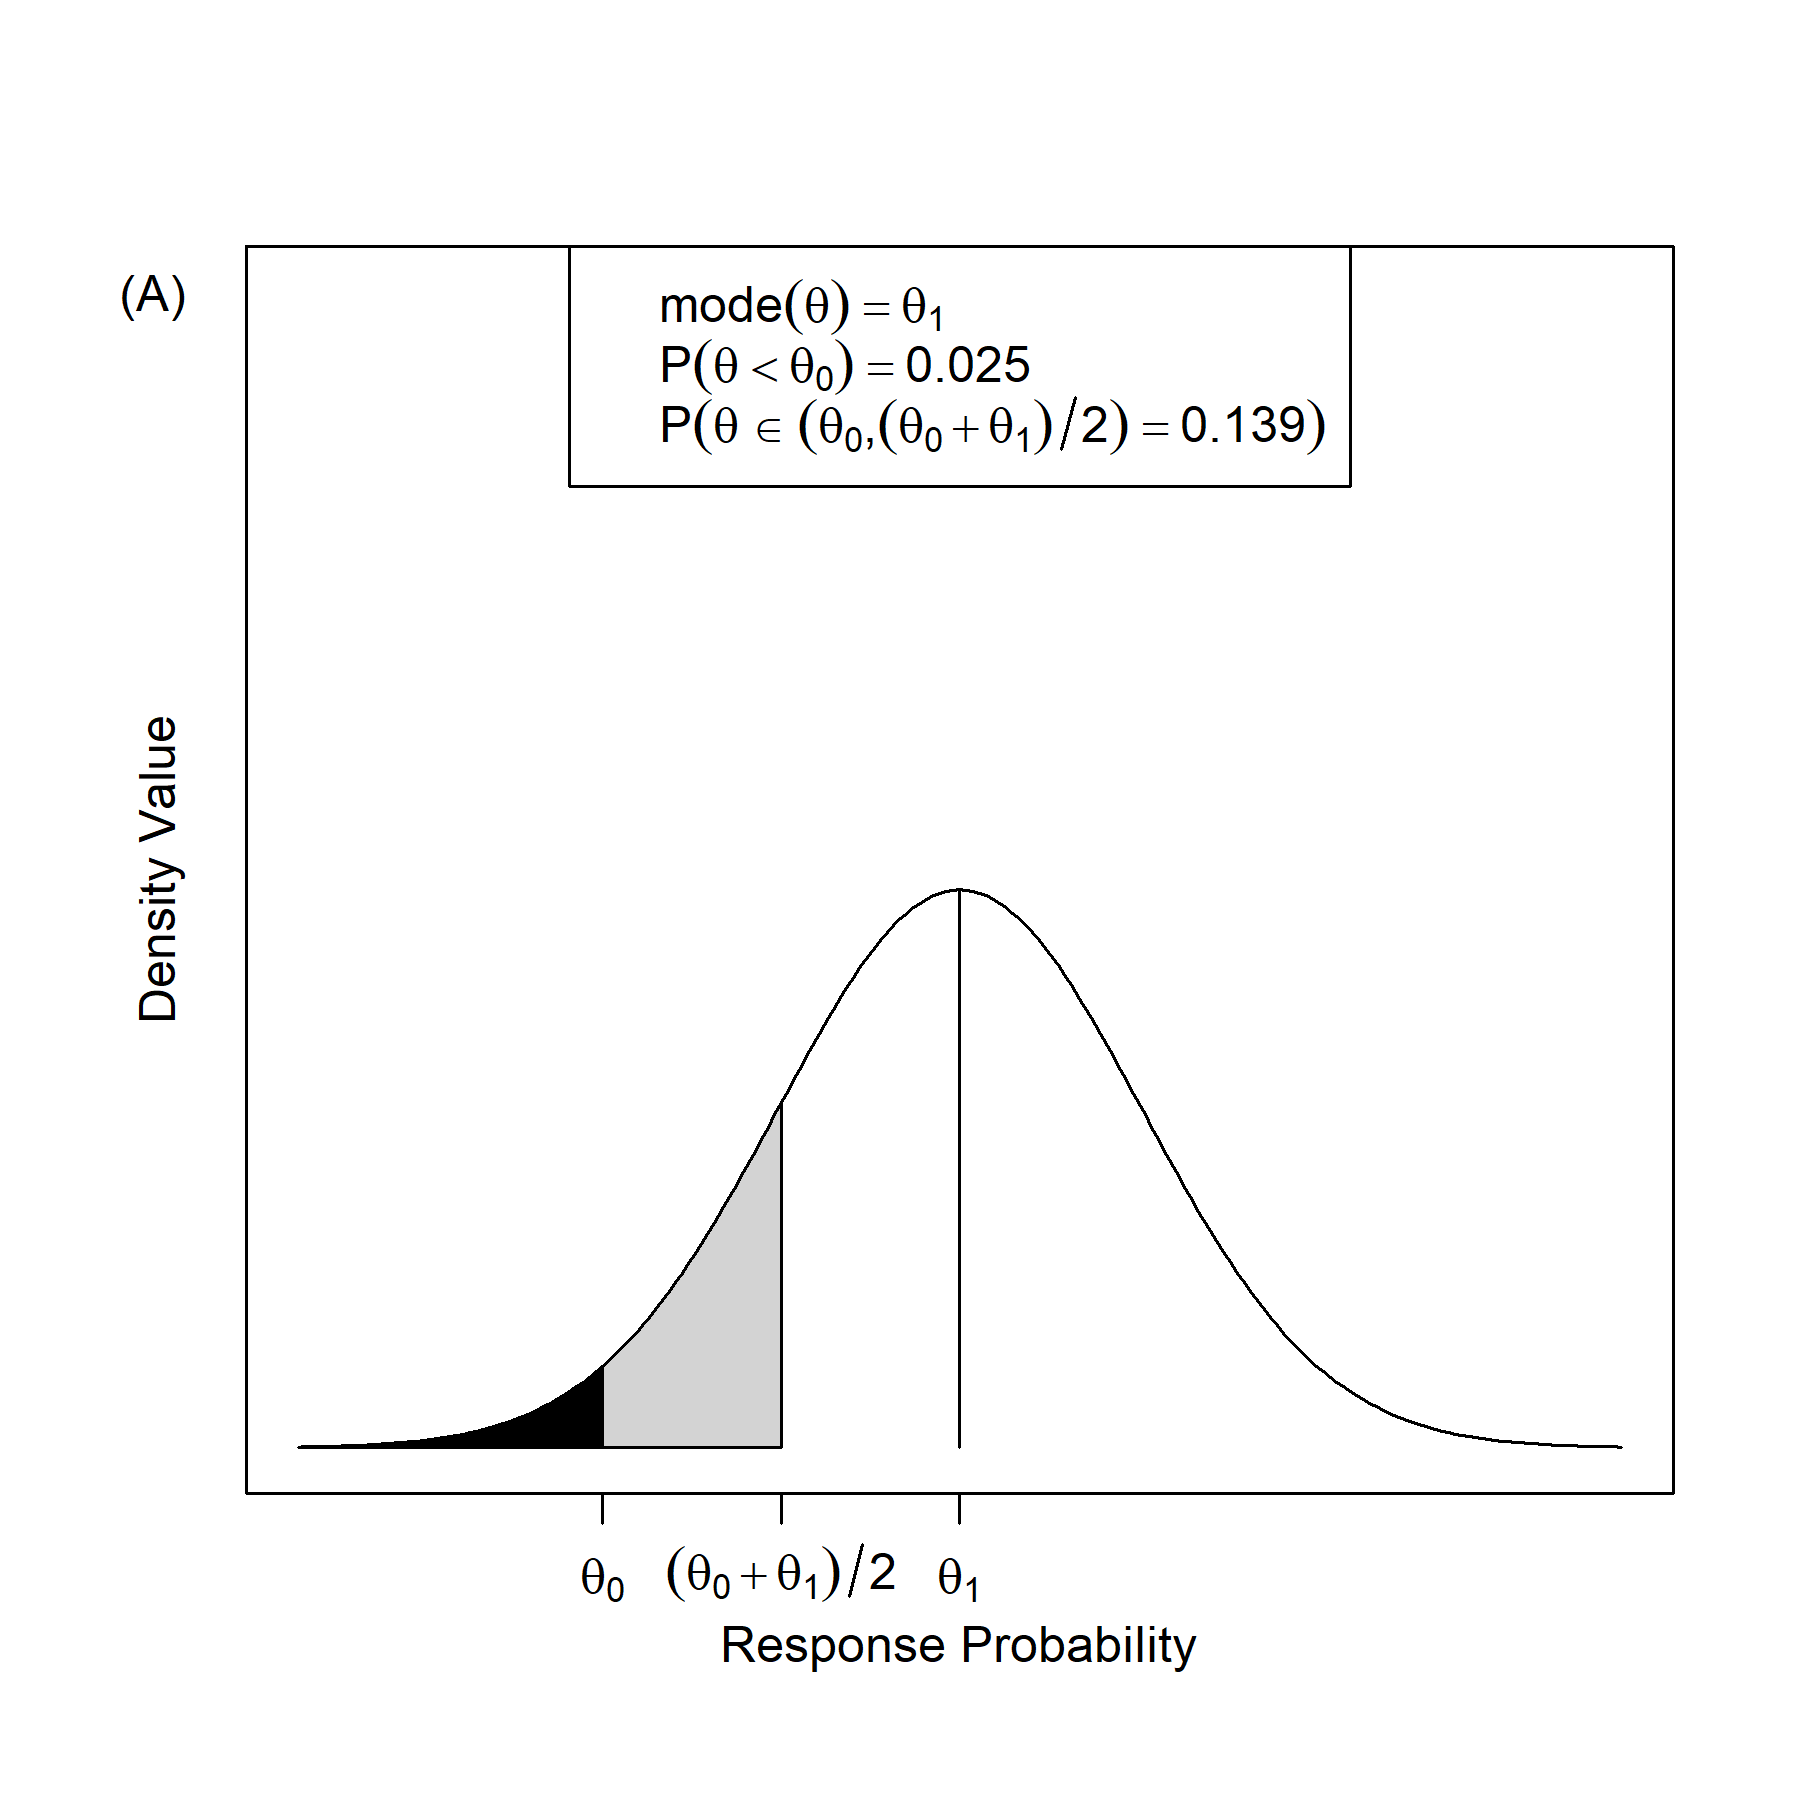
\includegraphics[width=3in]{figure1a.png}
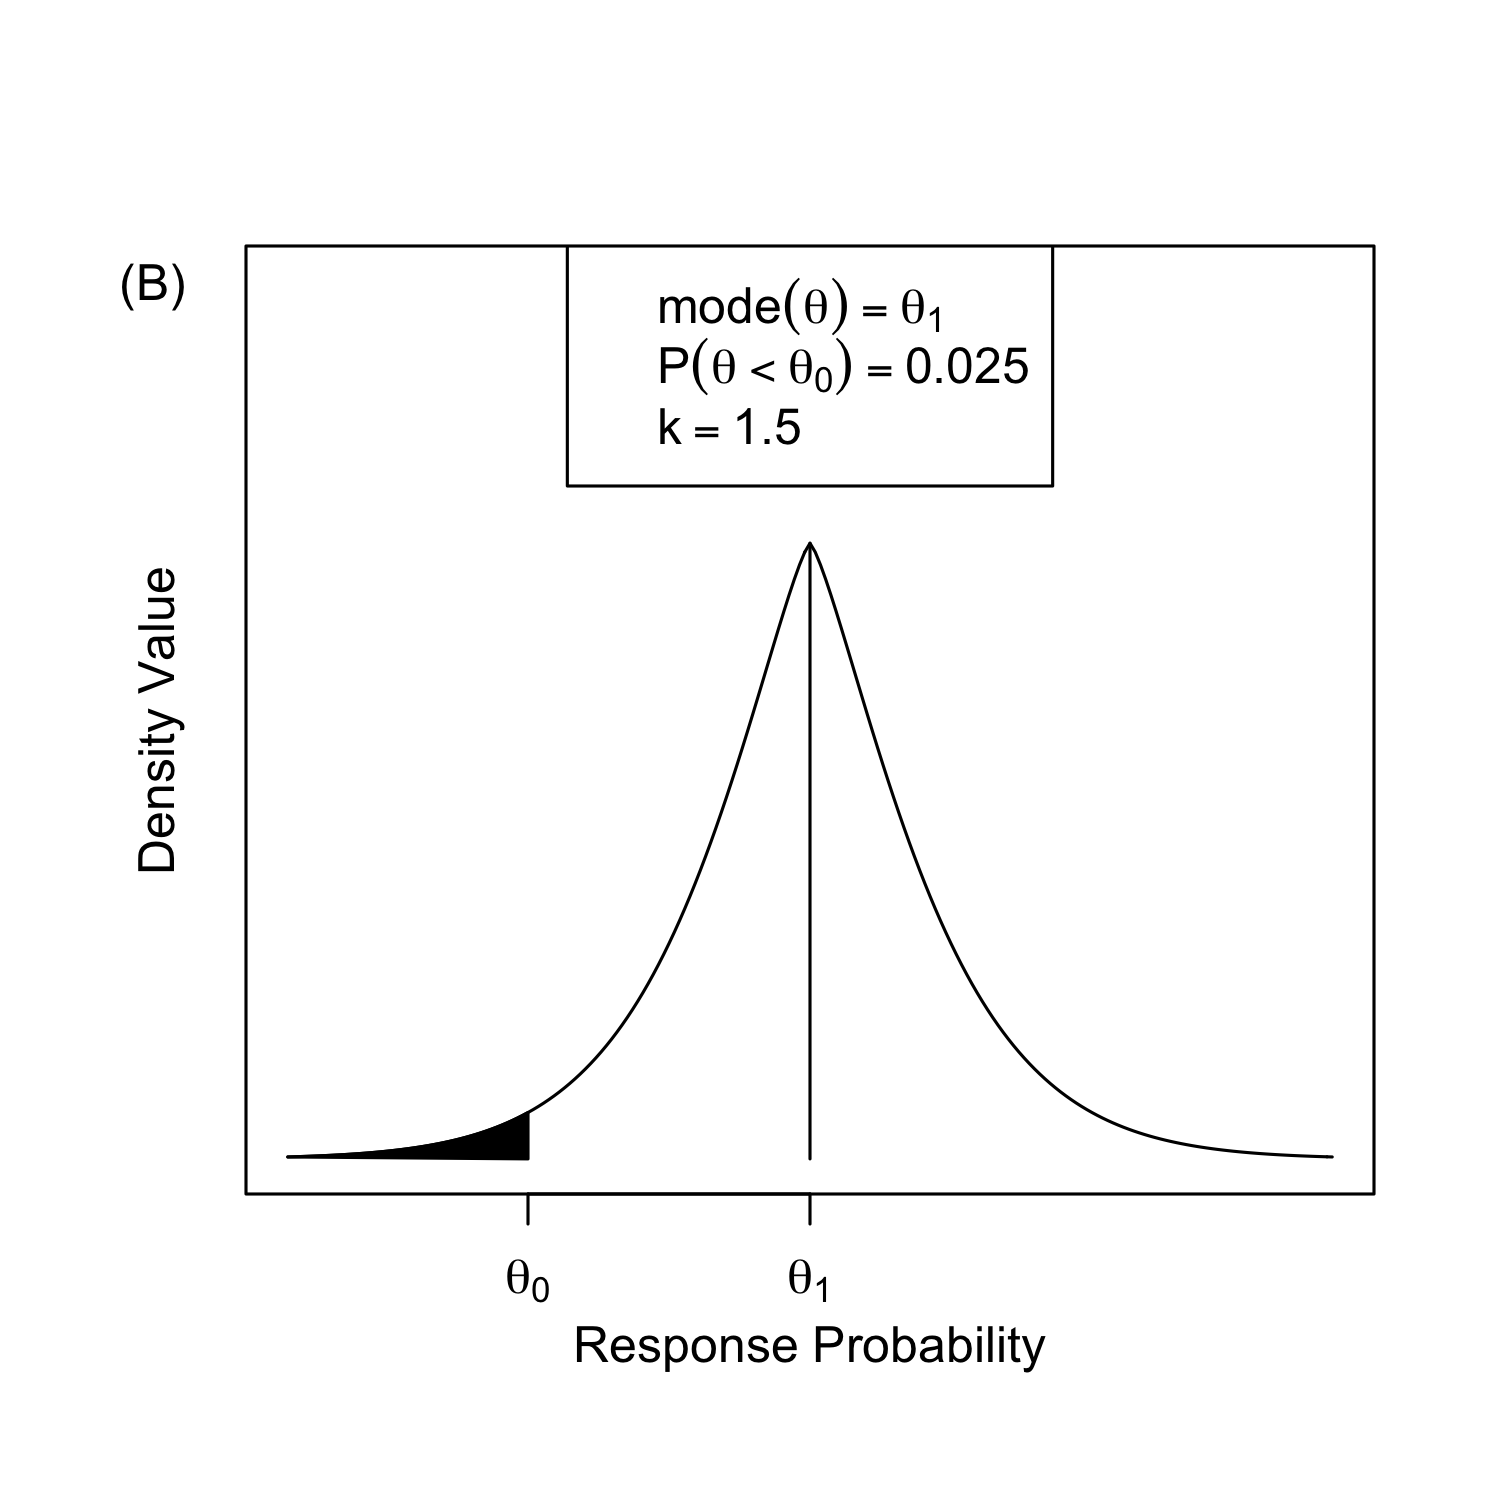
\includegraphics[width=3in]{figure1b.png}
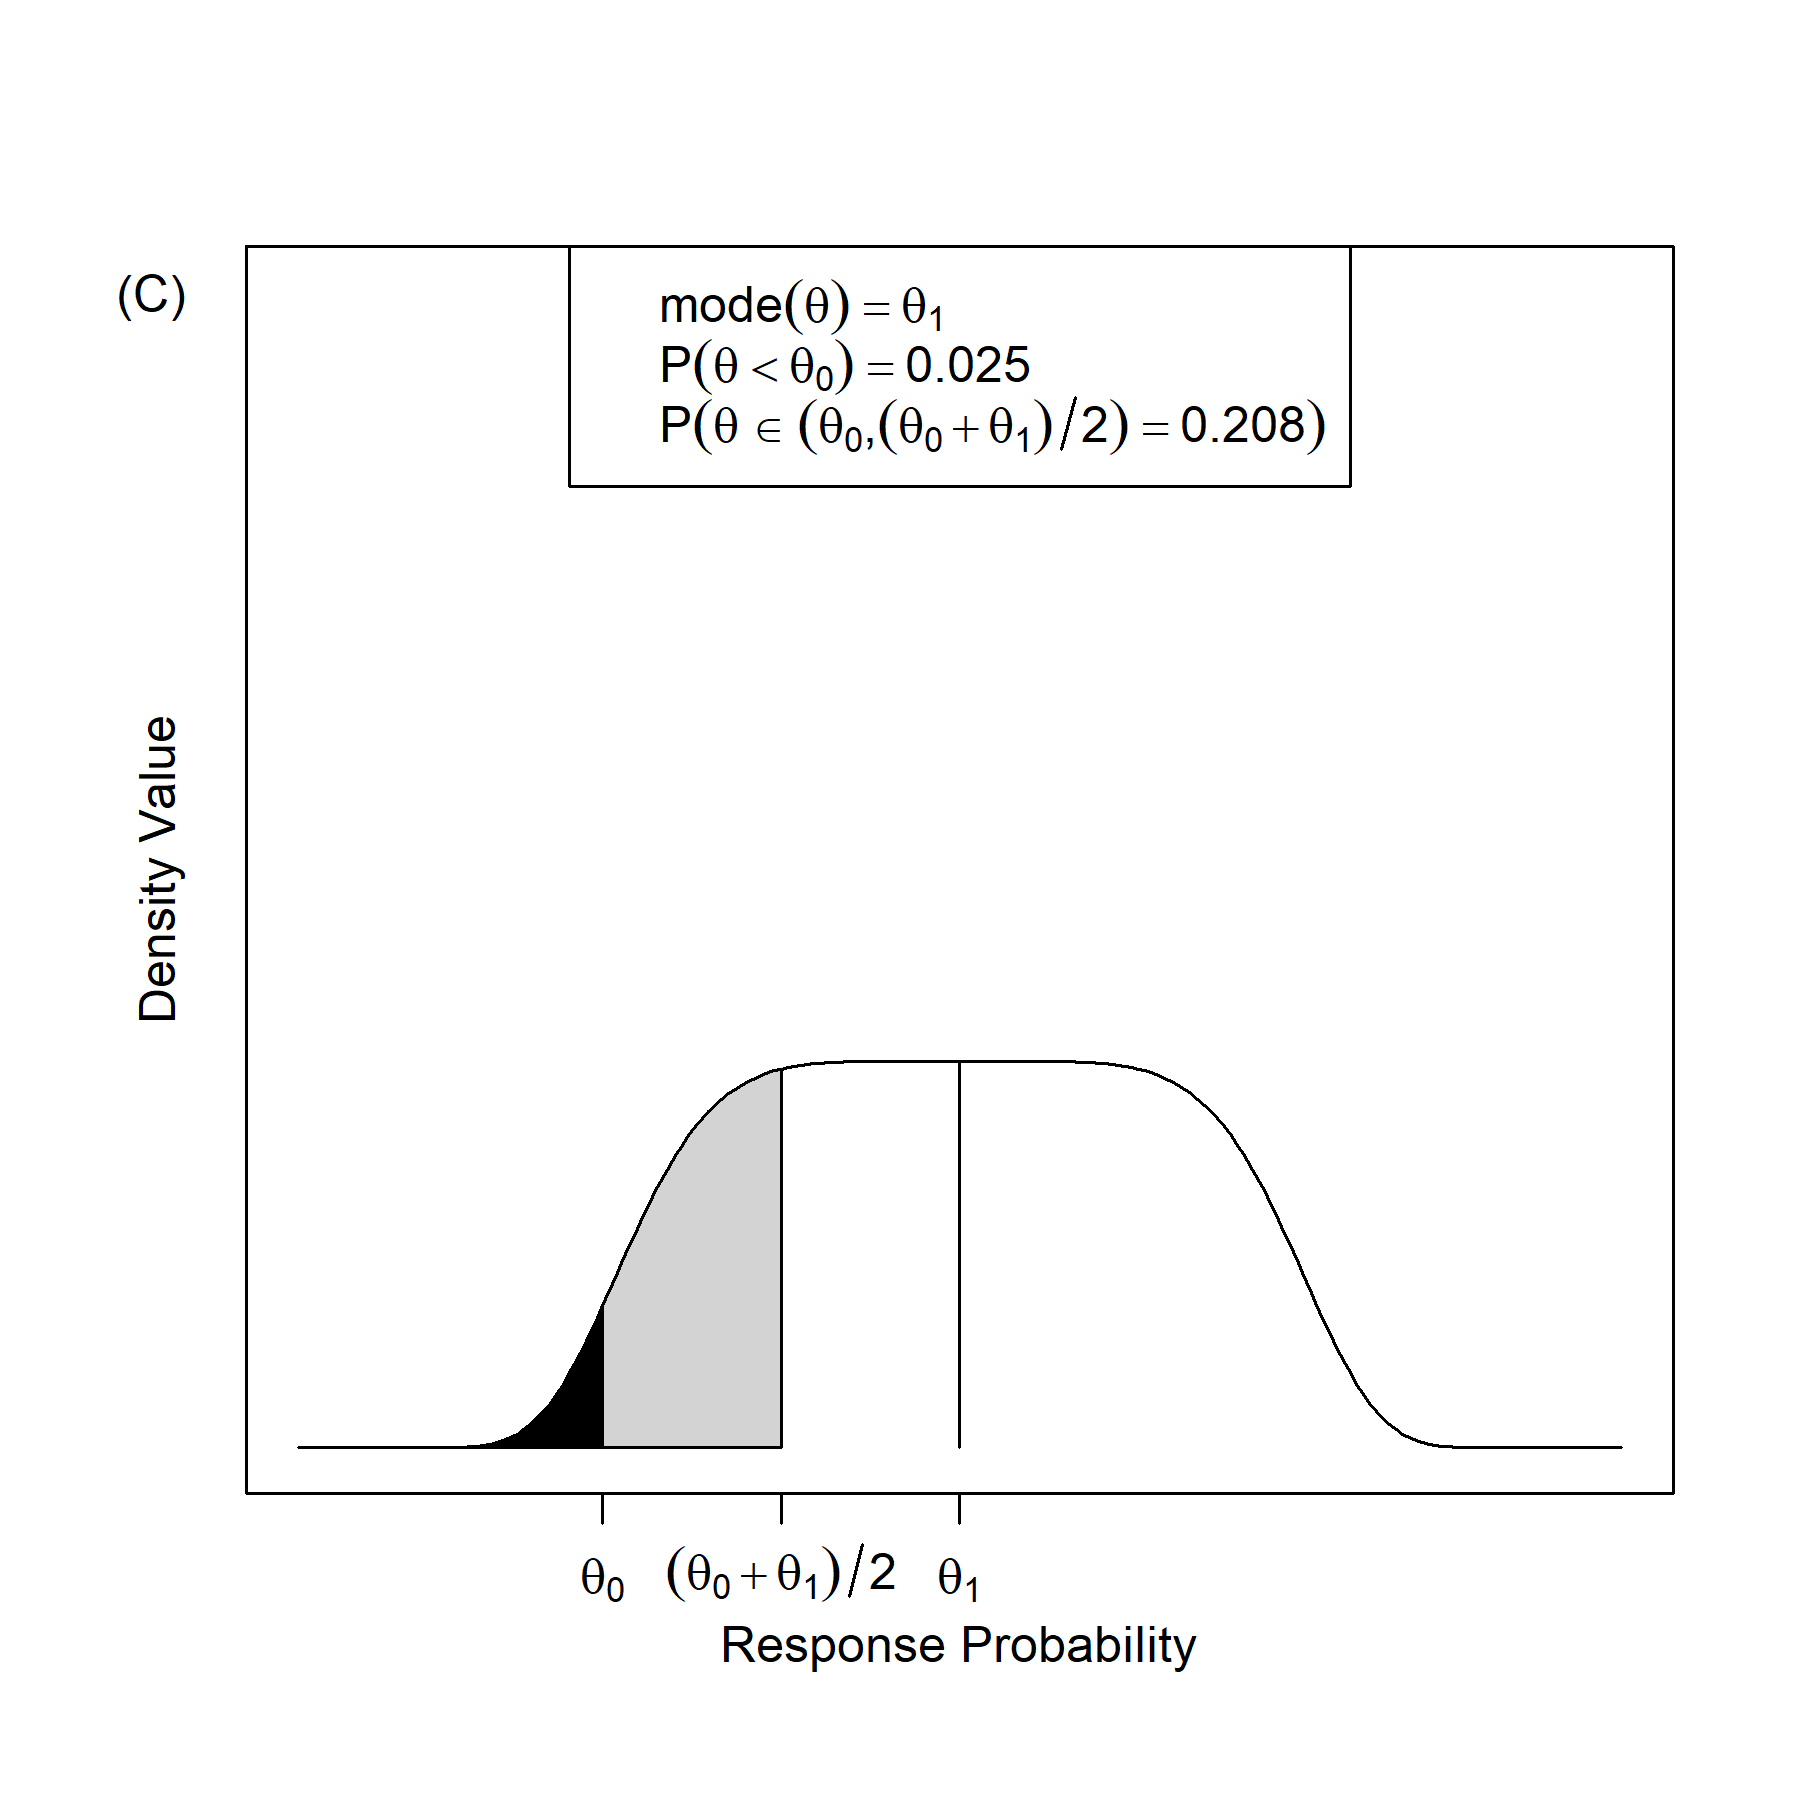
\includegraphics[width=3in]{figure1c.png}
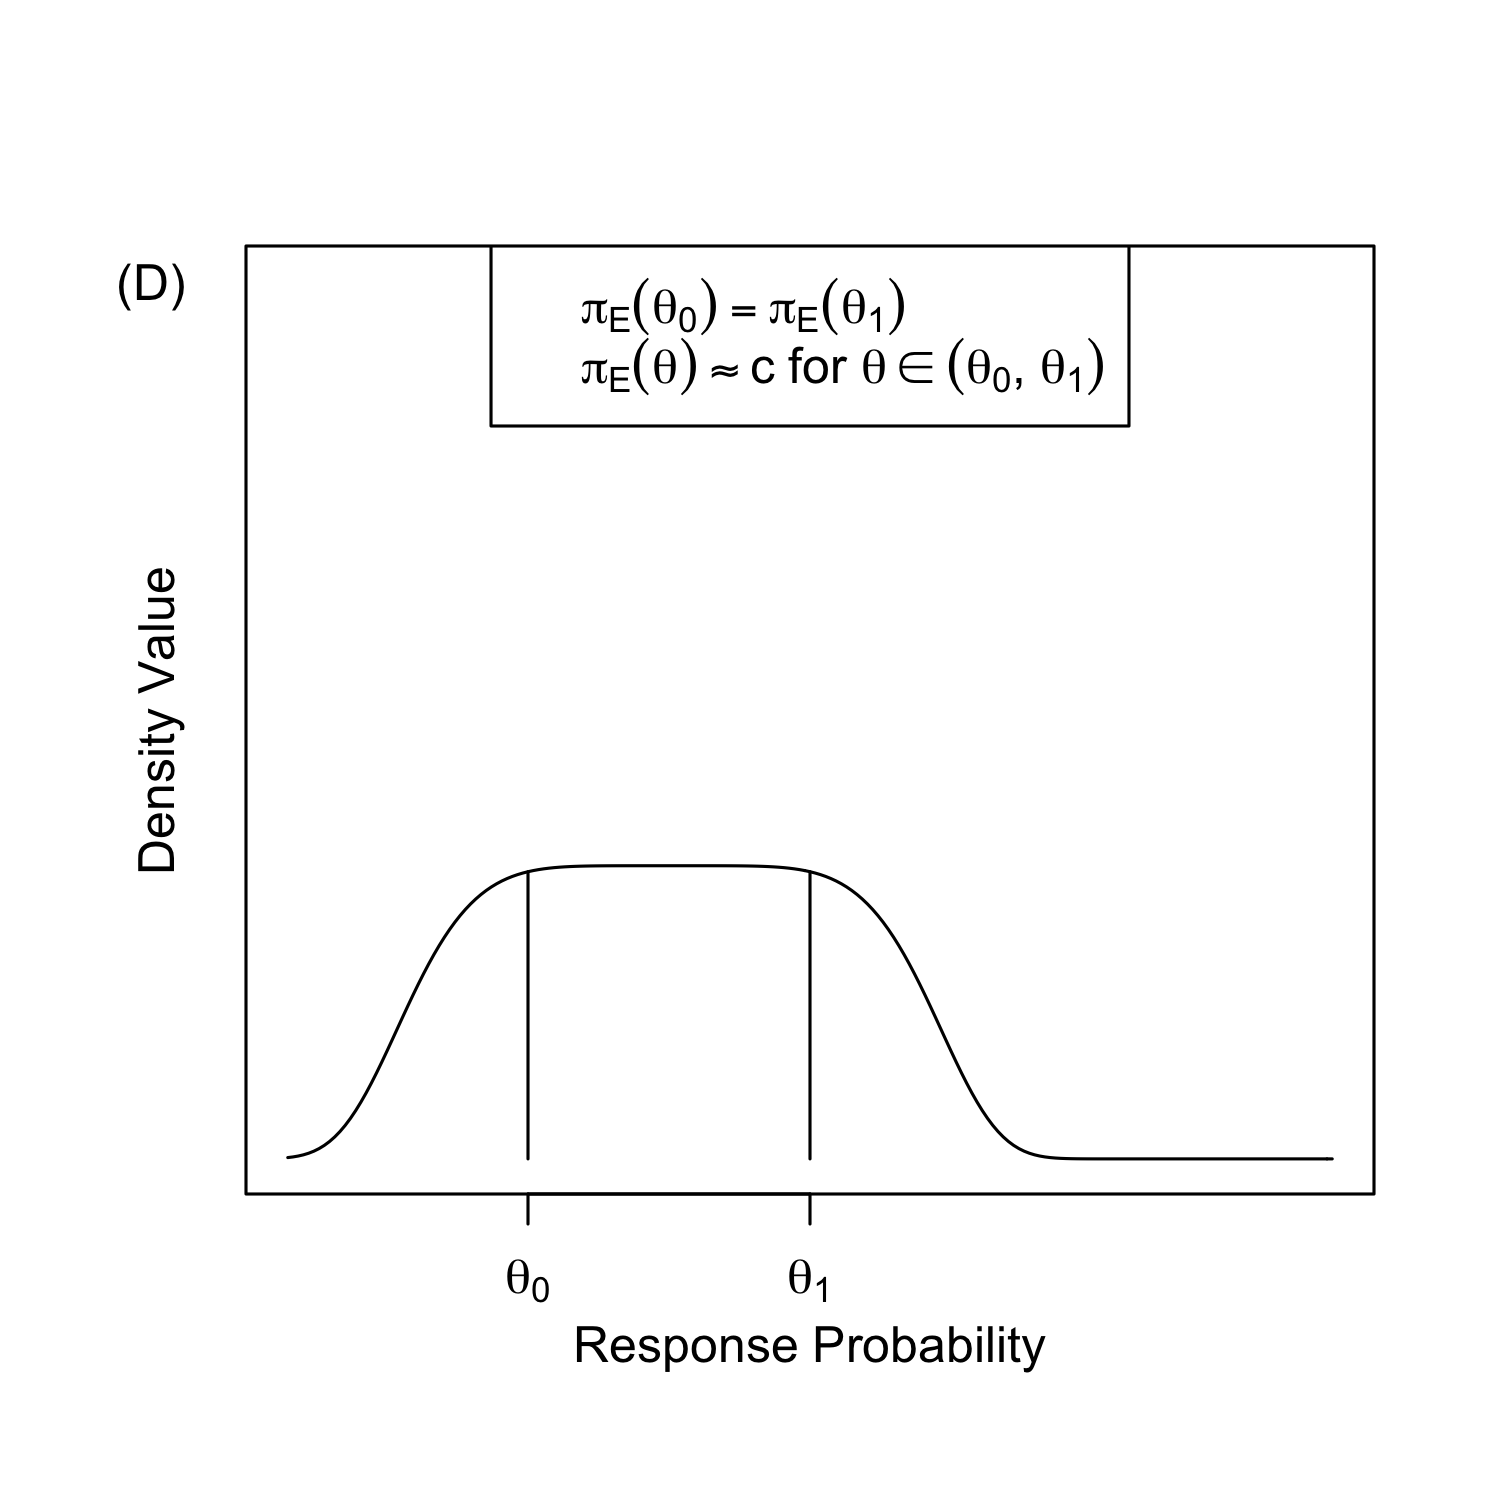
\includegraphics[width=3in]{figure1d.png}
\caption{A, Default enthusiastic prior. B, Concentrated enthusiastic prior. C, Flattened enthusiastic prior. D, Locally non-informative prior.}

\label{fig:figure1}
\end{center}
\end{figure}

{Panel B of Figure \ref{fig:figure1} presents a concentrated enthusiastic prior that satisfies 
the mode value and tail probability constraints given in Section~\ref{sec:MP}, and that has $k=1.5$ times the density value at the mode as compared to the default normal distribution. 
Increasing the density value at the mode translates to a more peaked distribution about the mode as compared to the default normal distribution (shown in Panel A). 
%
Panel C of Figure \ref{fig:figure1} presents a flattened enthusiastic prior that that satisfies the mode value and tail probability constraints given in Section~\ref{sec:MP}, and
that has $k=0.67$ times the density value at the mode as compared to the default normal distribution. This translates to a distribution that is significantly more flat about the mode value than the default normal distribution. 
%
Although we have focused on an enthusiastic prior in our discussion here, the same ideas apply to skeptical priors as well.
%
The approach we have proposed results in a unique flattened or concentrated prior.

The use of the scale factor $k$ corresponds to beliefs that reflect useful and nuanced perspectives for clinical trial decision making.
%
A concentrated skeptical prior views $\theta_0$ as being more likely than a data-driven (i.e. normally distributed via Bayesian CLT) perspective while still reflecting residual uncertainty that $\theta>\theta_1$.
%
This is a rational perspective for a monitoring prior since the skeptical viewpoint should give substantial preference to the null value.
%
Similarly, a flattened enthusiastic prior views $\theta_1$ as being less likely than a data-driven perspective while still reflecting residual uncertainty that $\theta<\theta_0$.
%
This is a rational perspective for a monitoring prior since even from an enthusiastic viewpoint, one may wish to reflect increased uncertainty regarding the likelihood of values at and around $\theta_1$.
%
While there is no \textit{correct} choice for the scale factor $k$ for either a skeptical or an enthusiastic prior, the author's choices
of $1.5$ and $0.67$ are relatively extreme perturbations from that afforded by the normal distribution and will be used henceforth to 
demonstrate the methodology proposed. 
	%
Lastly, we note that the default normal, flattened, and concentrated priors all can be truncated while maintaining the mode and tail 
probability constraints.
	%
This will be necessary when the parameter of interest has bounded support (e.g., $\theta$ is a response probability).
}

%\textcolor{red}{Note that I am changing the notation to what I think will make it more understandable but the graphs need to change too. I also struggle
%with how the definition given forces the distribution to be locally non-informative. It seems like the flattening criteria is what causes that. I recommend
%adding in the criteria $\pi_{NI}(\theta_0) \approx \pi_{NI}(\theta_1)$ \textit{as part of the definition} and revising this section accordingly. Another
%take on it would be to require $\pi_{NI}(\theta)$ be approximately equal for all $\theta \in \left[\theta_0,\theta_1\right]$ as a part of the definition.}
%\textcolor{blue}{
Lastly, we define a \textit{locally non-informative prior} as a prior that satisfies $\pi_{NI}(\theta_0) = \pi_{NI}(\theta_1)$, and where $\pi_{NI}(\theta)$ is approximately equal for all $\theta \in \left[\theta_0,\theta_1\right]$.
%%
%Let $\delta_{\theta} = 2\left(\theta_1 - \theta_0\right)$ (i.e., twice the difference between $\theta_1$ and $\theta_0$).
%%
%Specifically, we consider the locally non-informative prior, denoted by $\pi_{NI}(\theta)$, that suggests $\theta_{m}=\frac{\theta_0+\theta_1}{2}$ is the most likely value of $\theta$ 
%and that reflects the belief of an observer who is all but convinced that $\theta>\theta_{m} -\delta_{\theta}$ a priori and 
%all but convinced that $\theta < \theta_{m} +\delta_{\theta}$. 
%%
%Formally, this is defined as the prior $\pi_{NI}(\theta)$ satisfying
%\begin{equation}\label{eq:niprior}
%\text{argmax}_\theta~\pi_{NI}(\theta)=\frac{\theta_0+\theta_1}{2}\text{ and } 
%  P_{NI}\left(\theta>\theta_{m}-\delta_{\theta}\right)=P_{NI}\left(\theta< \theta_{m}+\delta_{\theta}\right) =1-\epsilon.
%\end{equation}
%This proposed prior is flattened such that there is $50\%$ more mass in the intervals $\left[\theta_{m}-\delta_{\theta},\theta_0\right]$ 
%and $\left[\theta_1,\theta_{m}+\delta_{\theta}\right]$ as compared to a normal distribution having the same mode value and tail probability constraints. 
%%
A locally non-informative prior is shown in Panel D of Figure \ref{fig:figure1}, and the technical definition is given in Web Appendix B.


%\item If $\gamma>1$ then the probability that $\theta\in(q,\frac{q+\mu}{2})$ increases and the concentration of $\theta$ around the mode value $\mu$ accordingly decreases, resulting in a flatter distribution around the mode value. 
%\item If $\gamma<1$ then the probability that $\theta\in(q,\frac{q+\mu}{2})$ decreases and the concentration of $\theta$ around the mode value $\mu$ accordingly increases, resulting in a more concentrated distribution around the mode value. 
%\item Flattening or concentrating the distribution around the mode value is useful for specifying monitoring priors that reflect varying opinions about the dispersion of $\theta$. 
%\item An example of parameterizing an enthusiastic prior with a $\mathcal{GN}_p(\tilde{\mu},q,\gamma)$ distribution is demonstrated in Figure \ref{fig:figure1}. 
%\item Choosing a concentrated distribution is appropriate when prior belief reflects a higher degree of certainty that $\theta$ is in a narrow range around $\theta_1$, while maintaining residual uncertainty that $\theta<\theta_0$. 
%\item This decreases the variance of the distribution, and can be seen to reflect a conservative opinion about the values of $\theta$. 
%\item Choosing a flattened distribution is appropriate when $\theta$ is more likely to be in a wide range of values around $\theta_1$, while maintaining the same residual uncertainty that $\theta<\theta_0$. 
%\item This increases the variance of the distribution, and can be seen to reflect a liberal opinion about the values of $\theta$. 

%\item The impact of flattening or concentrating the distribution of a monitoring prior on the operating characteristics of a trial is shown in Section \ref{sec:examples}.
%For example, consider creating skeptical and enthusiastic priors for a response probability on domain $[0,1]$, as $
%\pi_S(\theta)=\mathcal{GN}_{p=1-\epsilon,\Theta=[0,1]}(\tilde{\mu}=\theta_0,q=\theta_1,\gamma=1)$ and $
%\pi_E(\theta)=\mathcal{GN}_{p=\epsilon,\Theta=[0,1]}(\tilde{\mu}=\theta_1,q=\theta_0,\gamma=1)$ respectively.

%The normal and generalized normal family of distributions can be truncated to a restricted domain that reflects the research quantity of interest (e.g. a response probability on [0,1]).
%\subsubsection{Application to higher dimensions}
%Suppose the trial from Section \ref{sec:preliminaries} has added a control arm, and let $\eta_0$ and $\eta_1$ be the response proportions for a control and treatment group respectively. Suppose that the risk difference $\theta=\eta_1-\eta_0$ is the parameter of interest, and let $\eta_0$ be a nuisance parameter. Let $\delta_0$ denote a null risk difference and $\delta_1$ denote a highly efficacious risk difference.

\subsubsection{Incorporating Prior Information in the Monitoring Priors}\label{sec:incorporating}
The monitoring priors are constructed based on the quantities $\theta_0$ and $\theta_1$, as well as the definition of a compelling demonstration. 
%
As described previously, prior information may be directly used in the construction of the enthusiastic prior (e.g., choice of $\theta_1$).
%
It also may be desirable to incorporate prior information into the monitoring process when making a determination of when to stop enrollment 
early for efficacy.
%
To facilitate this, we introduce a procedure for modifying the monitoring process such that, if the enthusiastic prior is congruent with observed data, the degree of skepticism can be adaptively lessened.
	%
We propose incorporating prior information into the monitoring process for efficacy through constructing a mixture prior
from the skeptical and enthusiastic priors using a mixing weight that is constructed from measures of compatibility between the
observed data and the skeptical and enthusiastic priors. 
	%
We define the \textit{adaptive skeptical monitoring prior} as the mixture distribution	
\begin{equation}\label{eq:inference_prior}
	\pi_{AS}\left(\theta\right)=\omega\cdot\pi_{S}\left(\theta\right)+(1-\omega) \cdot \pi_E\left(\theta\right),
\end{equation}
where $\omega\in[0,1]$ is an adaptively determined mixing weight. Fixed choices of $\omega$ will be used as comparisons for the performance of the adaptive weight monitoring prior in Section \ref{sec:example2}. 


The adaptive mixing weight $\omega$ is determined by an assessment of prior-data conflict, proposed by \cite{Box1980}, derived using the prior predictive distribution of 
the data which is defined (in our case) using the skeptical and enthusiastic monitoring priors.
	%
The prior-predictive distribution for data $\mathbf{D}$ (also called the marginal likelihood) reflects the probability of observing $\mathbf{D}$ given 
the assumed prior distribution for $\theta$ and is defined formally as
\begin{equation}\label{eq:pred_dist}
p(\mathbf{D})=\int p(\bmath{D}|\theta)\pi(\theta)d\theta.
\end{equation}
	%
Let $\mathbf{D}_{\text{obs}}$ be the observed data at some point in time in an ongoing trial. 
	%
\textit{Box's p-value} is defined as the following:
%\begin{equation}
%p=P(p(y)\leq p(y_{obs}))
%\end{equation}
\begin{equation}\label{eq:box_p}
\psi({\mathbf{D}_{\text{obs}}})=\int {p(\mathbf{D})}  1[p(\mathbf{D})\leq p(\mathbf{D}_{\text{obs}})] d(\mathbf{D})
%\sum_{\mathbf{D}}p^{(h)}(\mathbf{D})1[p^{(h)}(\mathbf{D})\leq p^{(h)}(\mathbf{D}_{\text{obs}})]
\end{equation}
%which in the case of discrete data is equal to $\psi({\mathbf{D}_{\text{obs}}})=\sum_{\mathbf{D}}p(\mathbf{D})1[p(\mathbf{D})\leq p(\mathbf{D}_{\text{obs}})]$.
%
where $1[A]$ is an indicator that the event $A$ is true.

Box's p-value can be interpreted as the probability of observing data as or more extreme than $\mathbf{D}_{\text{obs}}$, given the predictive distribution. 
%
Small values of $\psi({\mathbf{D}_{\text{obs}}})$ indicate a lack of compatibility or congruency between the prior and the data. 
%
We propose using the skeptical and enthusiastic priors $\pi_S(\theta)$ and $\pi_E(\theta)$ to compute the quantities in \eqref{eq:pred_dist} and \eqref{eq:box_p} to create compatibility measurements $\psi^{(S)}(\mathbf{D}_{\text{obs}})$ and $\psi^{(E)}(\mathbf{D}_{\text{obs}})$ which are used to determine the mixing weight in \eqref{eq:inference_prior}. 
%
%If $\psi^{(E)}(\mathbf{D}_{\text{obs}})>\psi^{(S)}(\mathbf{D}_{\text{obs}})$, then the observed data are more consistent with the enthusiastic prior, which should be given a greater weight in the mixture. Similarly, if $\psi^{(S)}(\mathbf{D}_{\text{obs}})>\psi^{(E)}(\mathbf{D}_{\text{obs}})$ then the skeptical prior should be given a greater mixing weight.
A conservative choice of mixing weight which gives full weight to the skeptical prior (i.e. $\omega=1$) whenever $\psi^{(S)}(\mathbf{D}_{\text{obs}})\geq \psi^{(E)}(\mathbf{D}_{\text{obs}})$ is
\begin{equation}\label{eq:adaptive_prior}
\omega = 1 - \text{max}\left(0, \psi^{(E)}(\mathbf{D}_{\text{obs}})-\psi^{(S)}(\mathbf{D}_{\text{obs}})\right).
%\omega=\begin{cases} 
%      1 & \text{if } \psi^{(S)}(\mathbf{D}_{\text{obs}})\geq \psi^{(E)}(\mathbf{D}_{\text{obs}}) \\
%      1-\left[ \psi^{(E)}(\mathbf{D}_{\text{obs}})-\psi^{(S)}(\mathbf{D}_{\text{obs}}) \right] &\text{if } \psi^{(S)}(\mathbf{D}_{\text{obs}})< \psi^{(E)}(\mathbf{D}_{\text{obs}})
%   \end{cases}
\end{equation}
%
As can be seen, for the proposed approach the weight given to the enthusiastic component is the \textit{excess probability} in favor of the enthusiastic prior.
%
%Bayesian predictive model checking: model checking statistic and reference predictive distribution.




%

%


%Alternatively, $\omega$ can be informed by the data. Let $\hat{\theta}=\rmn{argmax} \{p(\bmath{D}|\theta)\}$ be the maximum likelihood estimator of $\theta$ given the data.
%%
%%%\begin{mydef}
%Define
%\begin{equation}\label{eq:dynamic_omega}
%\omega=\omega_{min}+(1-\omega_{min})\frac{\pi_S(\hat{\theta})}{\pi_S(\hat{\theta})+\pi_E(\hat{\theta})}
%\end{equation}
%as a mixing weight that dynamically gives preference to the prior that has the higher density evaluated at $\hat{\theta}$ with a minimum weight $\omega_{min}$ given to the skeptical component with $\omega_{min}\in[0,1]$.
%%%\end{mydef}

\subsubsection{Inference Priors}\label{sec:inferencepriors}
The purpose of the inference prior is to synthesize posterior inferences from the disparate skeptical and enthusiastic perspectives to 
facilitate interpretation of the data once it has been obtained. 
%
The skeptical and enthusiastic monitoring priors defined in Section~\ref{sec:MP} represent extreme but plausible 
beliefs about $\theta$.
%
While analysis with these priors provides a rational perspective from which one can determine whether interim data 
are sufficient to cease enrolling patients, the belief of most stakeholders will likely fall somewhere between the 
two perspectives.
%
Thus, when interpreting the final data once in hand, intermediate perspectives should be considered.
%
To that end, we define an inference prior through mixing the two monitoring priors, with the optional addition of a locally non-informative prior to provide added robustness.

{
Define the inference prior as
\begin{equation}\label{eq:3partmix}
\pi(\theta)=\omega_S\cdot \pi_S(\theta)+\omega_E\cdot\pi_E(\theta)+\omega_{NI}\cdot\pi_{NI}(\theta)
\end{equation}
where $\omega_S+\omega_E+\omega_{NI}=1$ and each weight is non-negative. 
	%
One may take $\omega_{NI}=0$ and fixed value of $\omega_S=\omega_E=1/2$ to obtain an \textit{agnostic} inference prior since it 
gives equal weight to the skeptical and enthusiastic components (see Section \ref{sec:example1}).
%
%This type of inference prior is demonstrated in Section \ref{sec:example1}.
}

{
Alternatively, an adaptive inference prior is obtained as follows.
	%
One first computes the quantities $\psi^{(S)}(\mathbf{D}_{\text{obs}})$, $\psi^{(E)}(\mathbf{D}_{\text{obs}})$, and $\psi^{(NI)}(\mathbf{D}_{\text{obs}})$ using the priors $\pi_S(\theta)$, 
$\pi_E(\theta)$, and $\pi_{NI}(\theta)$, respectively, based on Box's p-value as given in \eqref{eq:box_p}. 
	%
Each of $\psi^{(S)}(\mathbf{D}_{\text{obs}})$, $\psi^{(E)}(\mathbf{D}_{\text{obs}})$, and $\psi^{(NI)}(\mathbf{D}_{\text{obs}})$ characterizes compatibility of the data with the respective prior.
	%
Our goal is to create a mixture prior which gives more weight to the skeptical (or enthusiastic) prior in situations where the data are highly compatible 
with that prior and that favors the locally non-informative prior if data exhibit low compatibility with both the skeptical and enthusiastic priors.
	%
 To that end, we propose transforming $\psi^{(NI)}(\mathbf{D}_{\text{obs}})$ to obtain $\tilde{\psi}^{(NI)}(\mathbf{D}_{\text{obs}})$ which is defined as
\begin{equation}\label{eq:3partmix_ni}
\tilde{\psi}^{(NI)}(\mathbf{D}_{\text{obs}})=\text{max}\left[0,\psi^{(NI)}(\mathbf{D}_{\text{obs}})-\text{max}\left(\psi^{(S)}(\mathbf{D}_{\text{obs}}),\psi^{(E)}(\mathbf{D}_{\text{obs}})\right)\right].
%\begin{cases} 
%      \psi^{(NI)}(\mathbf{D}_{\text{obs}})-\text{max}(\psi^{(S)}(\mathbf{D}_{\text{obs}}),\psi^{(E)}(\mathbf{D}_{\text{obs}})) \text{ if }\\ \psi^{(NI)}(\mathbf{D}_{\text{obs}})>\text{max}(\psi^{(S)}(\mathbf{D}_{\text{obs}}),\psi^{(E)}(\mathbf{D}_{\text{obs}}))\\
%      0 \text{ if } \\\psi^{(NI)}(\mathbf{D}_{\text{obs}})\leq\text{max}(\psi^{(S)}(\mathbf{D}_{\text{obs}}),\psi^{(E)}(\mathbf{D}_{\text{obs}}))
%   \end{cases}.
\end{equation}	
	%
We then let the mixing weights $\omega^{(E)}$, $\omega^{(S)}$, and $\omega^{(NI)}$ be the normalized values of $\psi^{(E)}(\mathbf{D}_{\text{obs}})$, $\psi^{(S)}(\mathbf{D}_{\text{obs}})$, and $\tilde{\psi}^{(NI)}(\mathbf{D}_{\text{obs}})$ so that their sum is unity.
	%
This type of inference prior is demonstrated in Section \ref{sec:example2}.
}

\subsubsection{Prior Specification for Nuisance Parameters}\label{sec:cond_marg}
%\textcolor{red}{This section confuses me a good deal. In reference to the figure (and hypotheses to be tested), what are $\eta_0$ and $\eta_1$. These things have not be defined.
%	%
%Second, it seems like one would elicit $\pi(\theta)$ to satisfy tail probability constraints but it is not clear how or why they would do that for $\pi(\eta|\theta)$ since 
%this is a conditional distribution for nuisance parameters. 
%	%
%Third, why would $\pi(\eta|\theta)$ be a default skeptical prior as stated in the figure caption. That does not make sense as $\eta$ has nothing to do with the 
%hypotheses being tested.
%	%
%I think this entire section needs to be rewritten and perhaps simulations redone. It is hard for me to tell based on what is written here.
%}
	%
Often there are additional parameters besides the treatment effect $\theta$ that are not of primary interest (i.e. nuisance parameters).
%
It is necessary to elicit a prior distribution $\pi(\theta,\eta)$ for all unknown quantities.
%
The marginal-conditional factorization of the joint prior $\pi(\theta,\eta)=\pi(\theta)\times\pi(\eta|\theta)$ allows direct elicitation of the marginal prior on the treatment effect and provides the ability to incorporate prior information on the nuisance parameters through their conditional distribution given $\theta$.
%
The prior for $\pi(\theta)$ will be a generalized normal distribution that satisfies the aforementioned mode value and tail probability constraints.
%
We propose to define $\pi(\eta|\theta)$ as a generalized normal distribution, with parameters chosen based on shape of the conditional distribution evaluated at the most likely value of $\pi(\theta)$. For example, if $\pi_S(\theta)$ is a skeptical prior, then the location, shape, and scale parameters for a generalized normal distribution for $\pi(\eta|\theta)$ will be chosen based on $\pi(\eta|\theta=\theta_0)$. The location parameter will be the most likely value of $\eta$ when $\theta=\theta_0$ (e.g. $\text{mode}(\eta|\theta=\theta_0)=\eta_0)$, and shape and scale parameters will be chosen to reflect a reasonable amount of uncertainty regarding $\eta$. 
%

If the parameters $\theta$ and $\eta$ are assumed to be independent, then the joint prior can be factored as $\pi(\theta,\eta)=\pi(\theta)\times\pi(\eta)$ and the priors $\pi(\theta)$ and $\pi(\eta)$ can be elicited separately.
%
In some cases this is not possible. For example, suppose that $\theta$ is the risk difference between response probabilities of a treatment group and the control group, and denote the response probability in the control group by $\eta$.
%
In this case $\theta$ and $\eta$  are linked through constrained support (e.g. $0\leq \theta+\eta\leq 1)$. Such a prior specification is demonstrated in Figure \ref{fig:figure5}, and Section \ref{sec:example2model} uses this representation of the joint prior. Panel A shows the marginal distribution $\pi(\theta)$, Panel B shows the conditional distribution $\pi(\eta|\theta=\theta_0)$, and Panel C shows the joint prior $\pi(\theta,\eta)$. In this example, the conditional distribution $\pi(\eta|\theta)$ will look very similar to the marginal distribution of $\pi(\eta)$ except at the boundaries of the parameter space.

\begin{figure}\begin{center}
%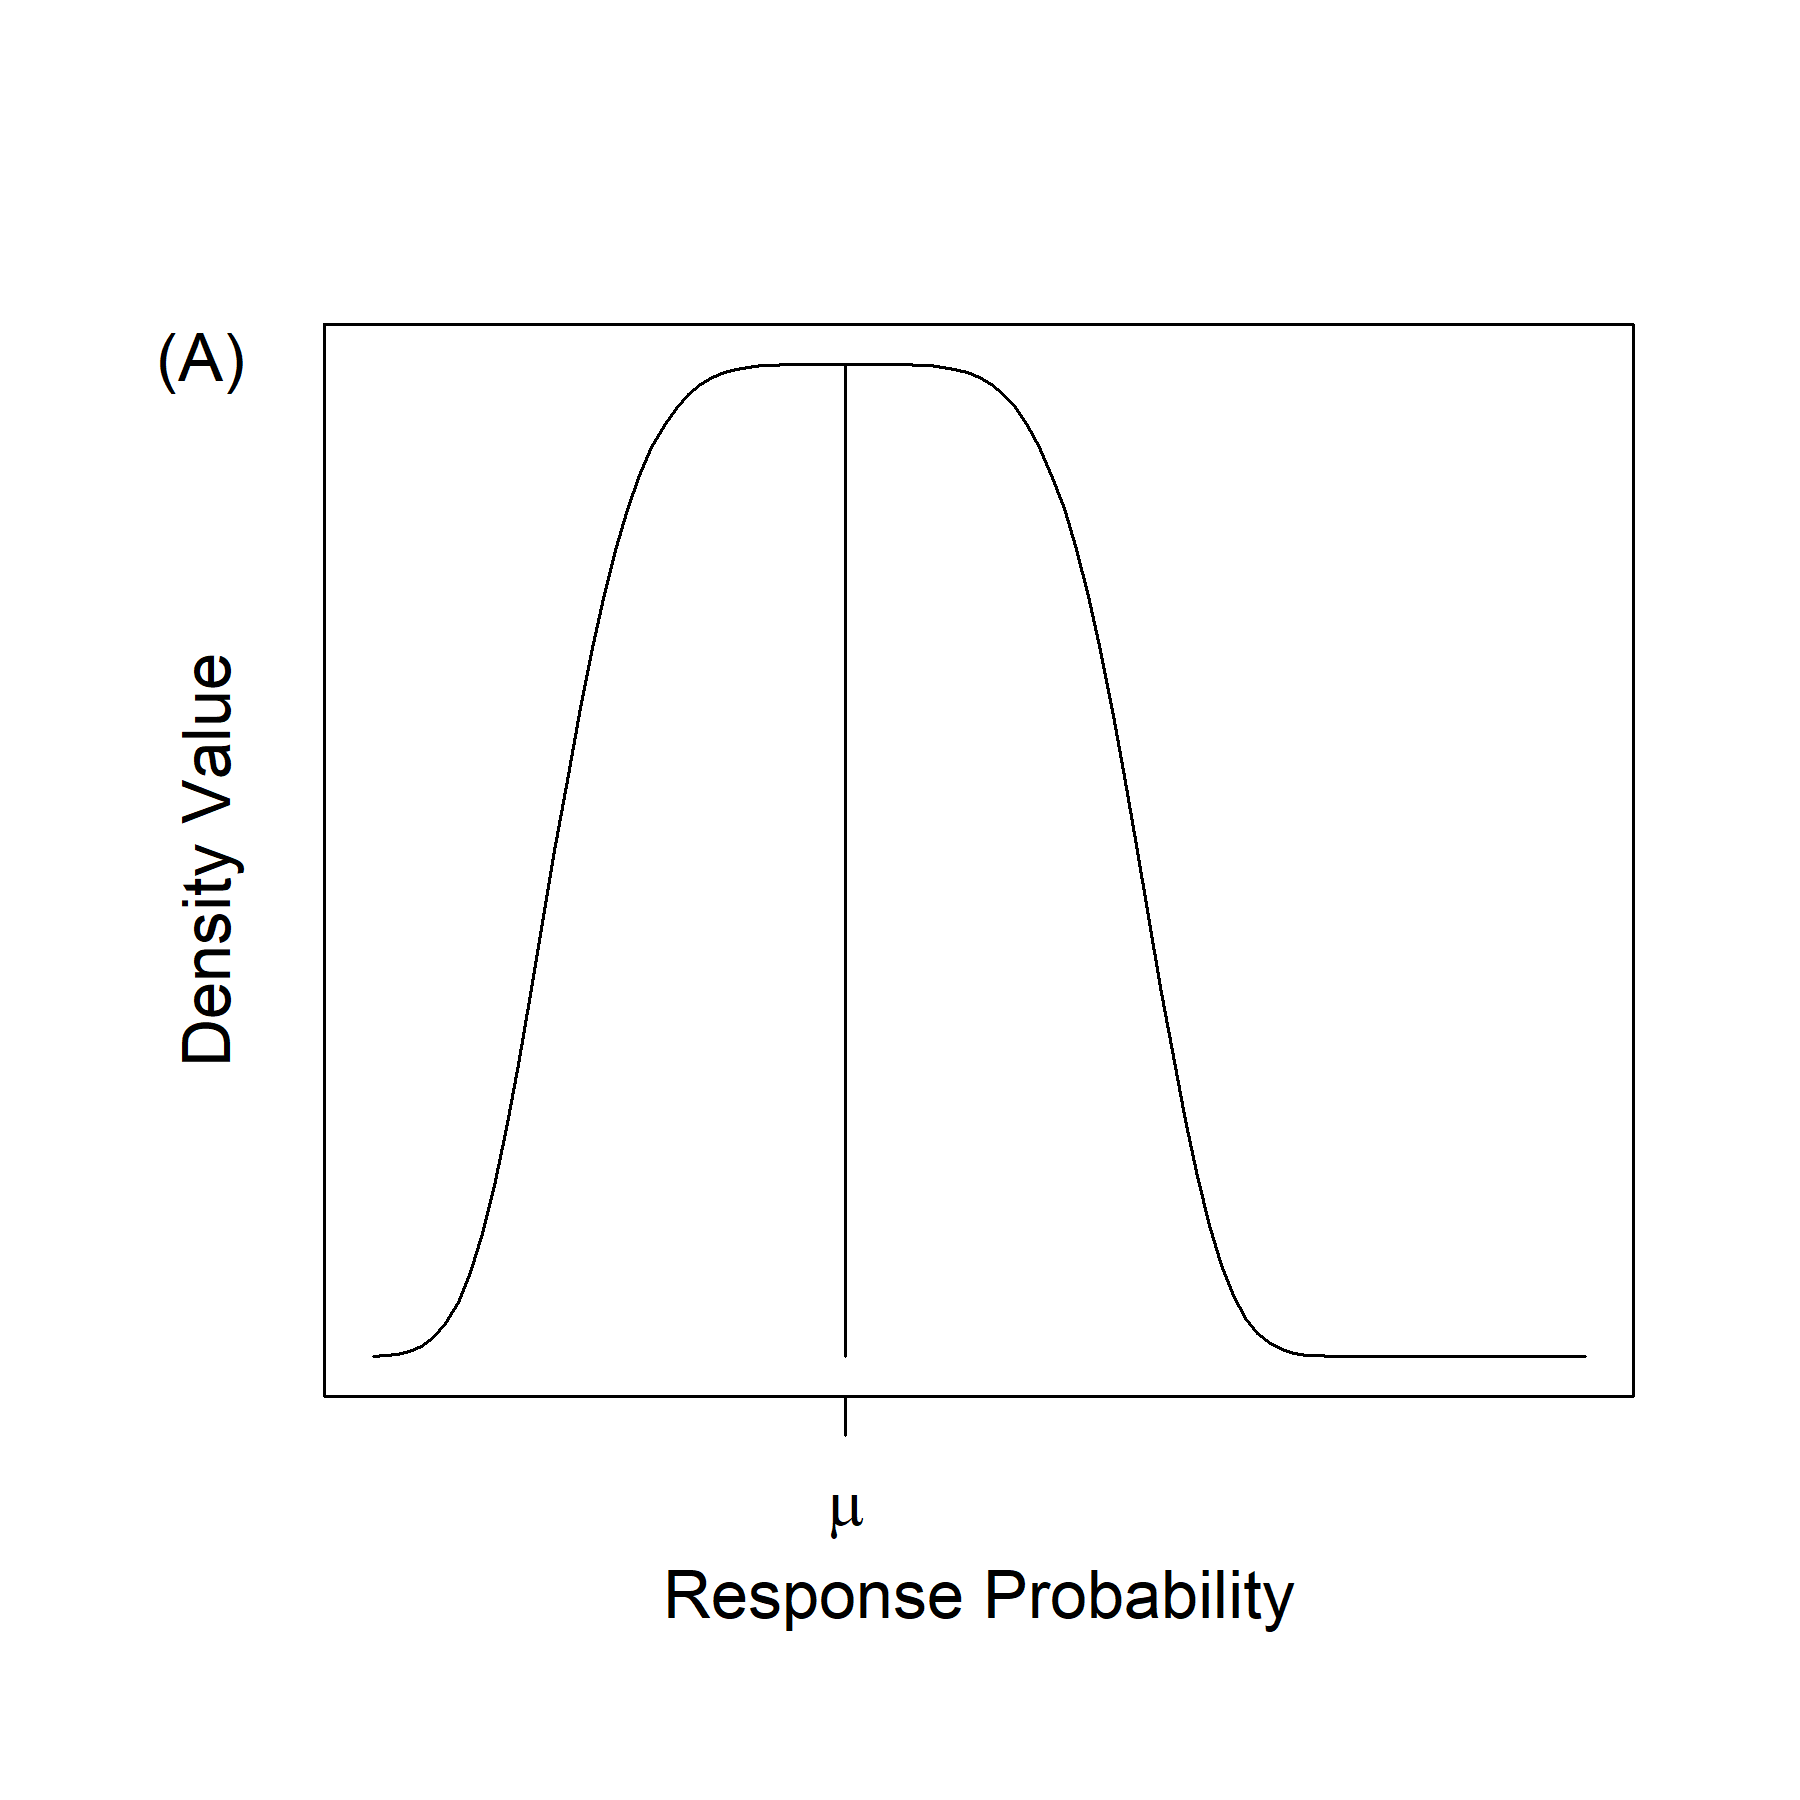
\includegraphics[width=6in]{figure5c.png}
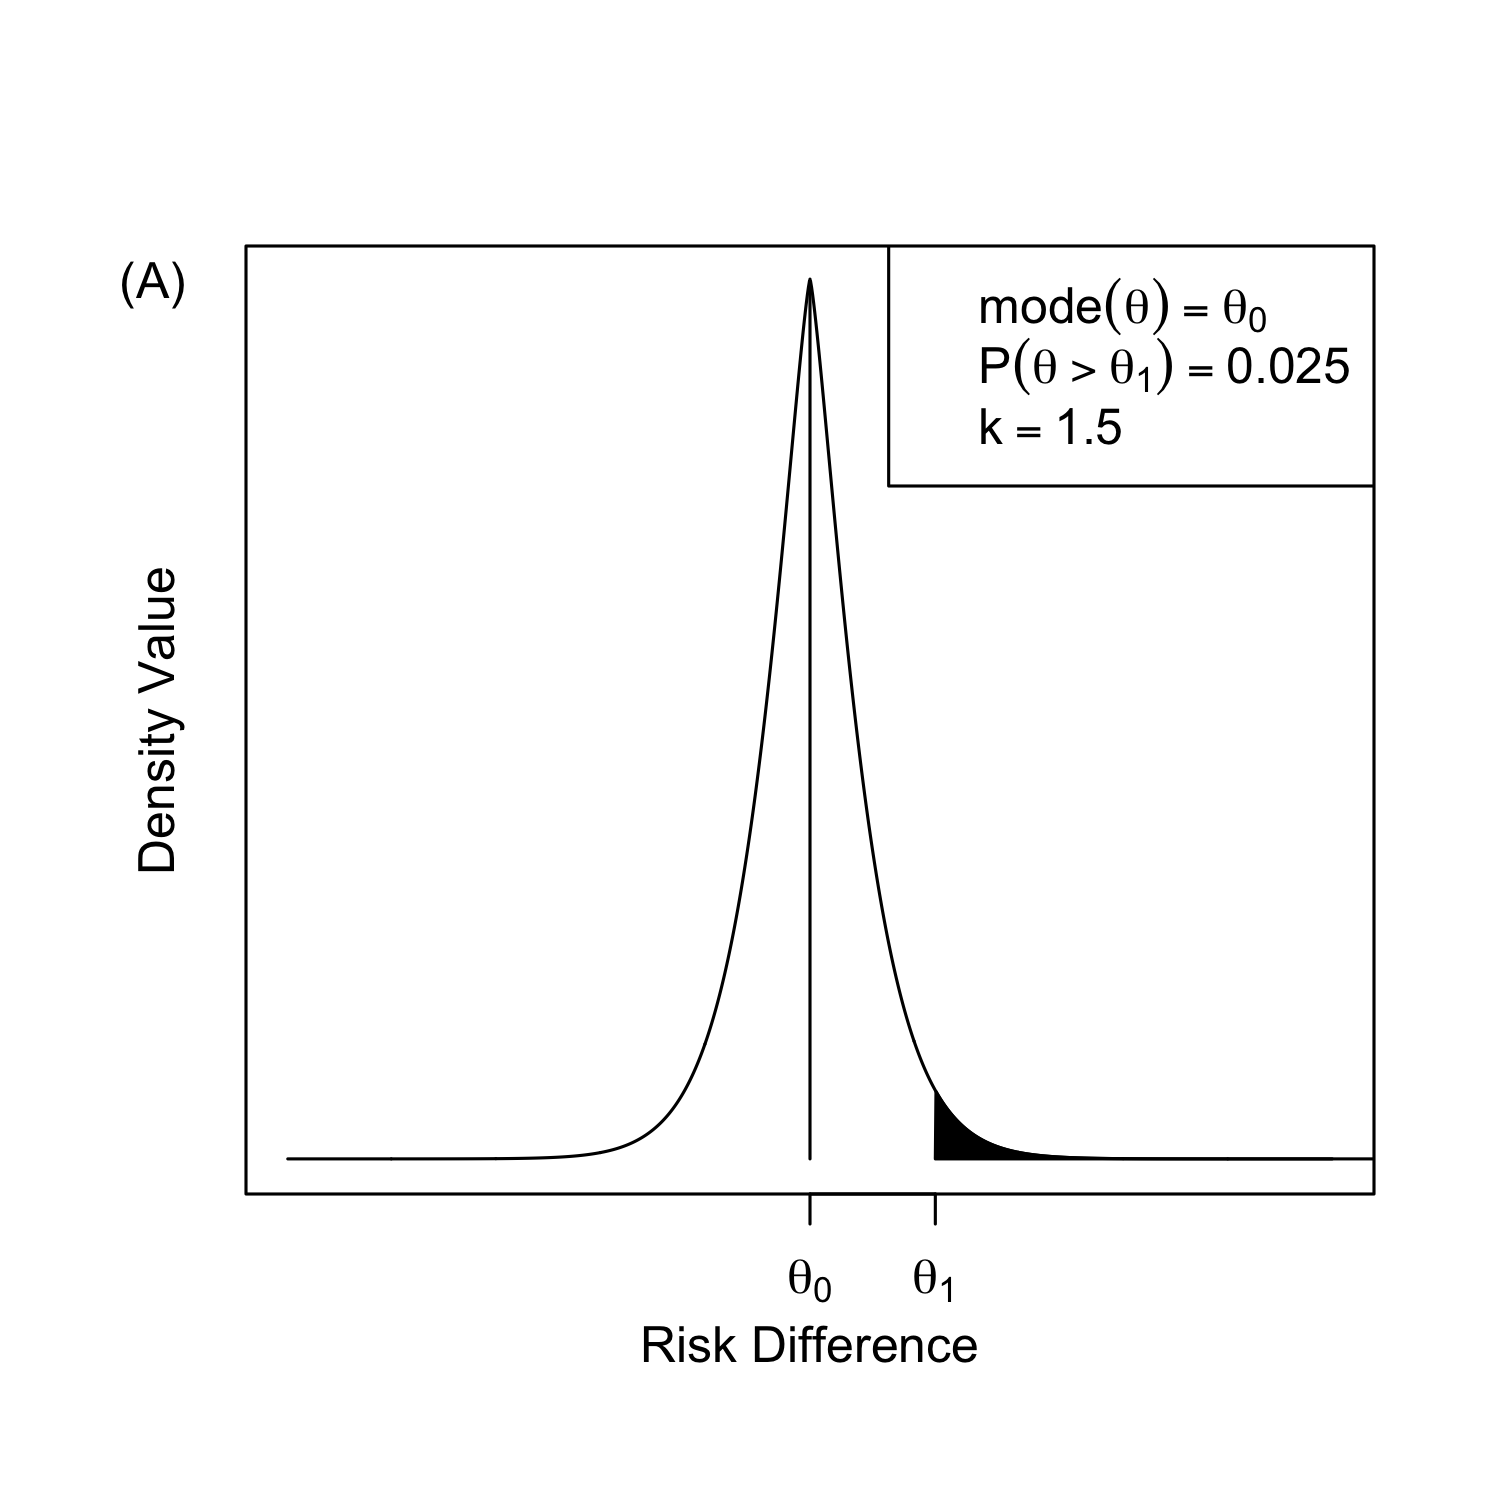
\includegraphics[width=3in]{figure5a_NEW.png}
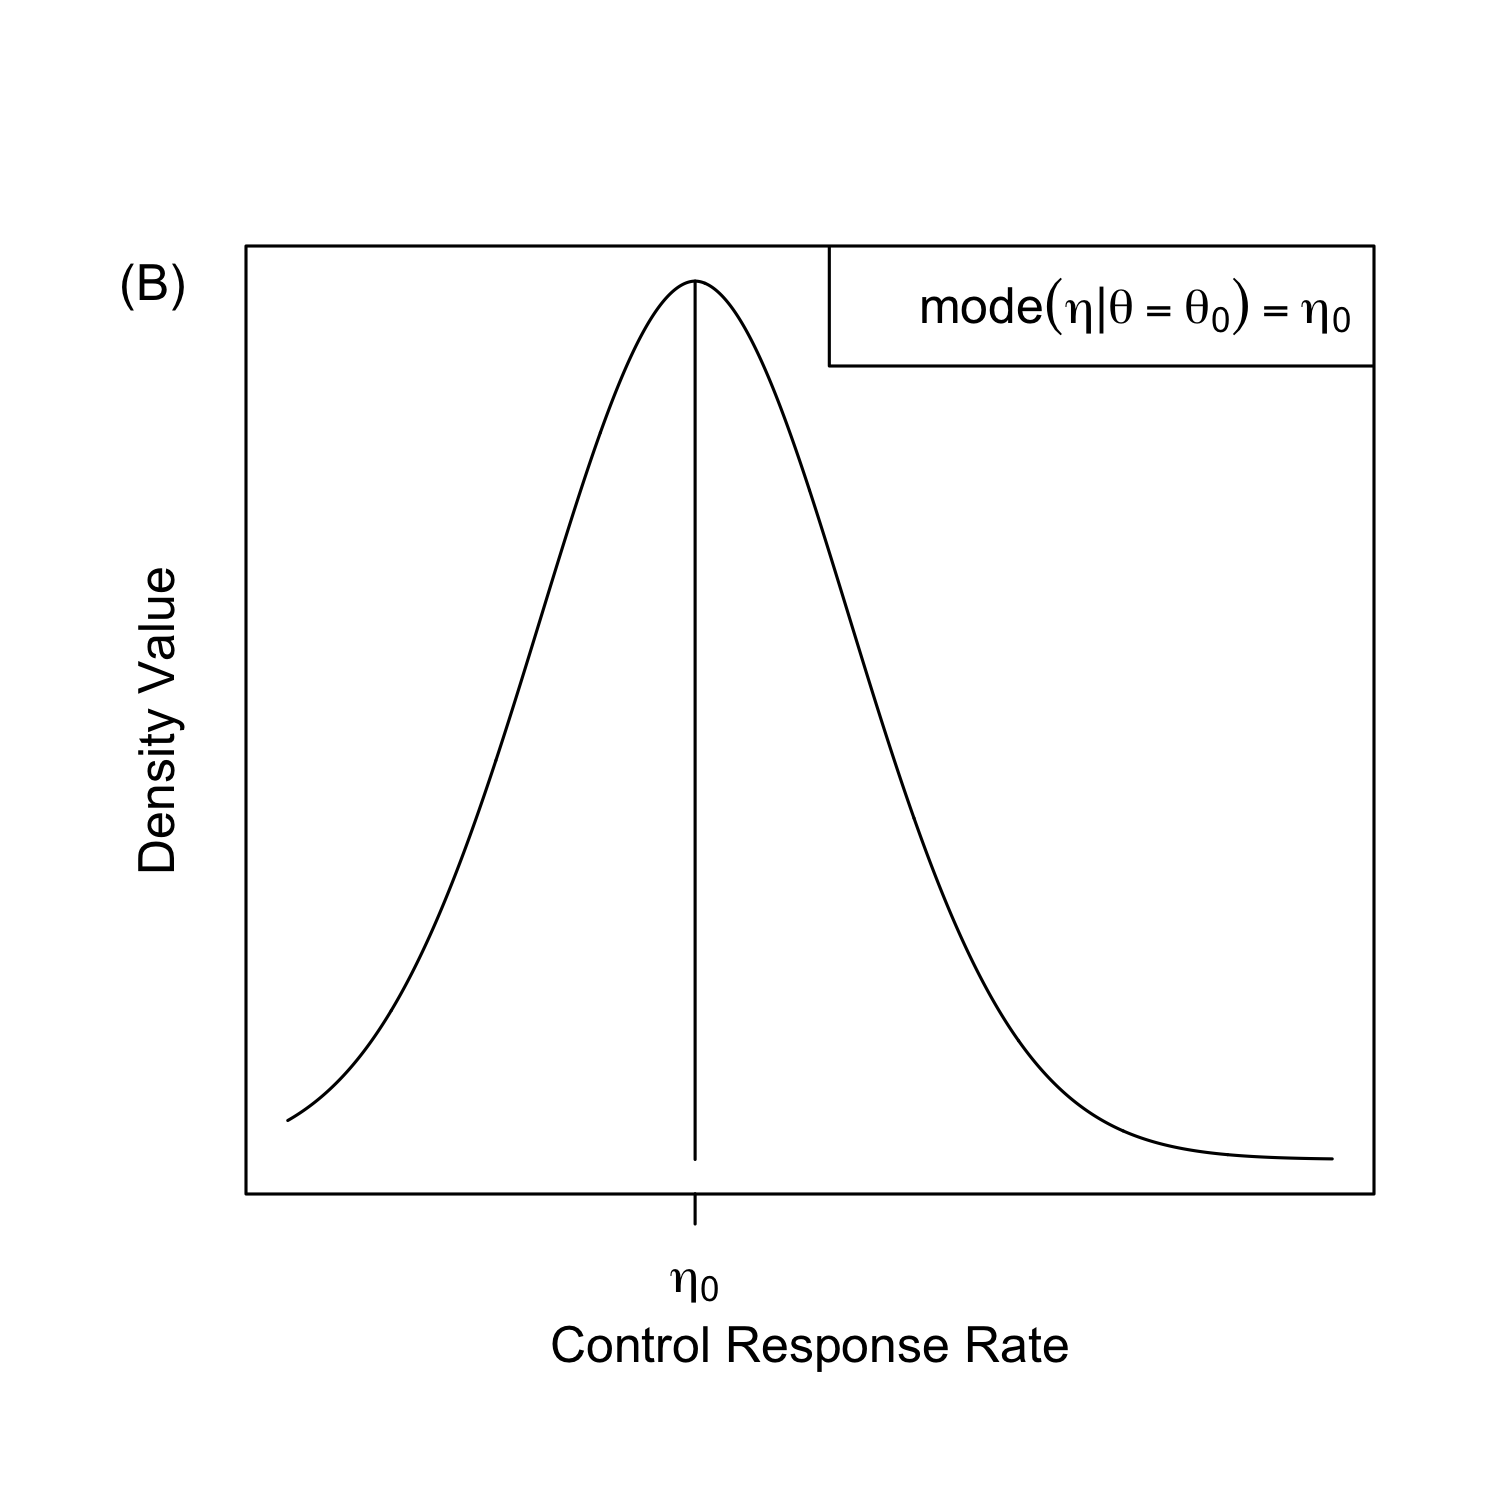
\includegraphics[width=3in]{figure5b_NEW.png}
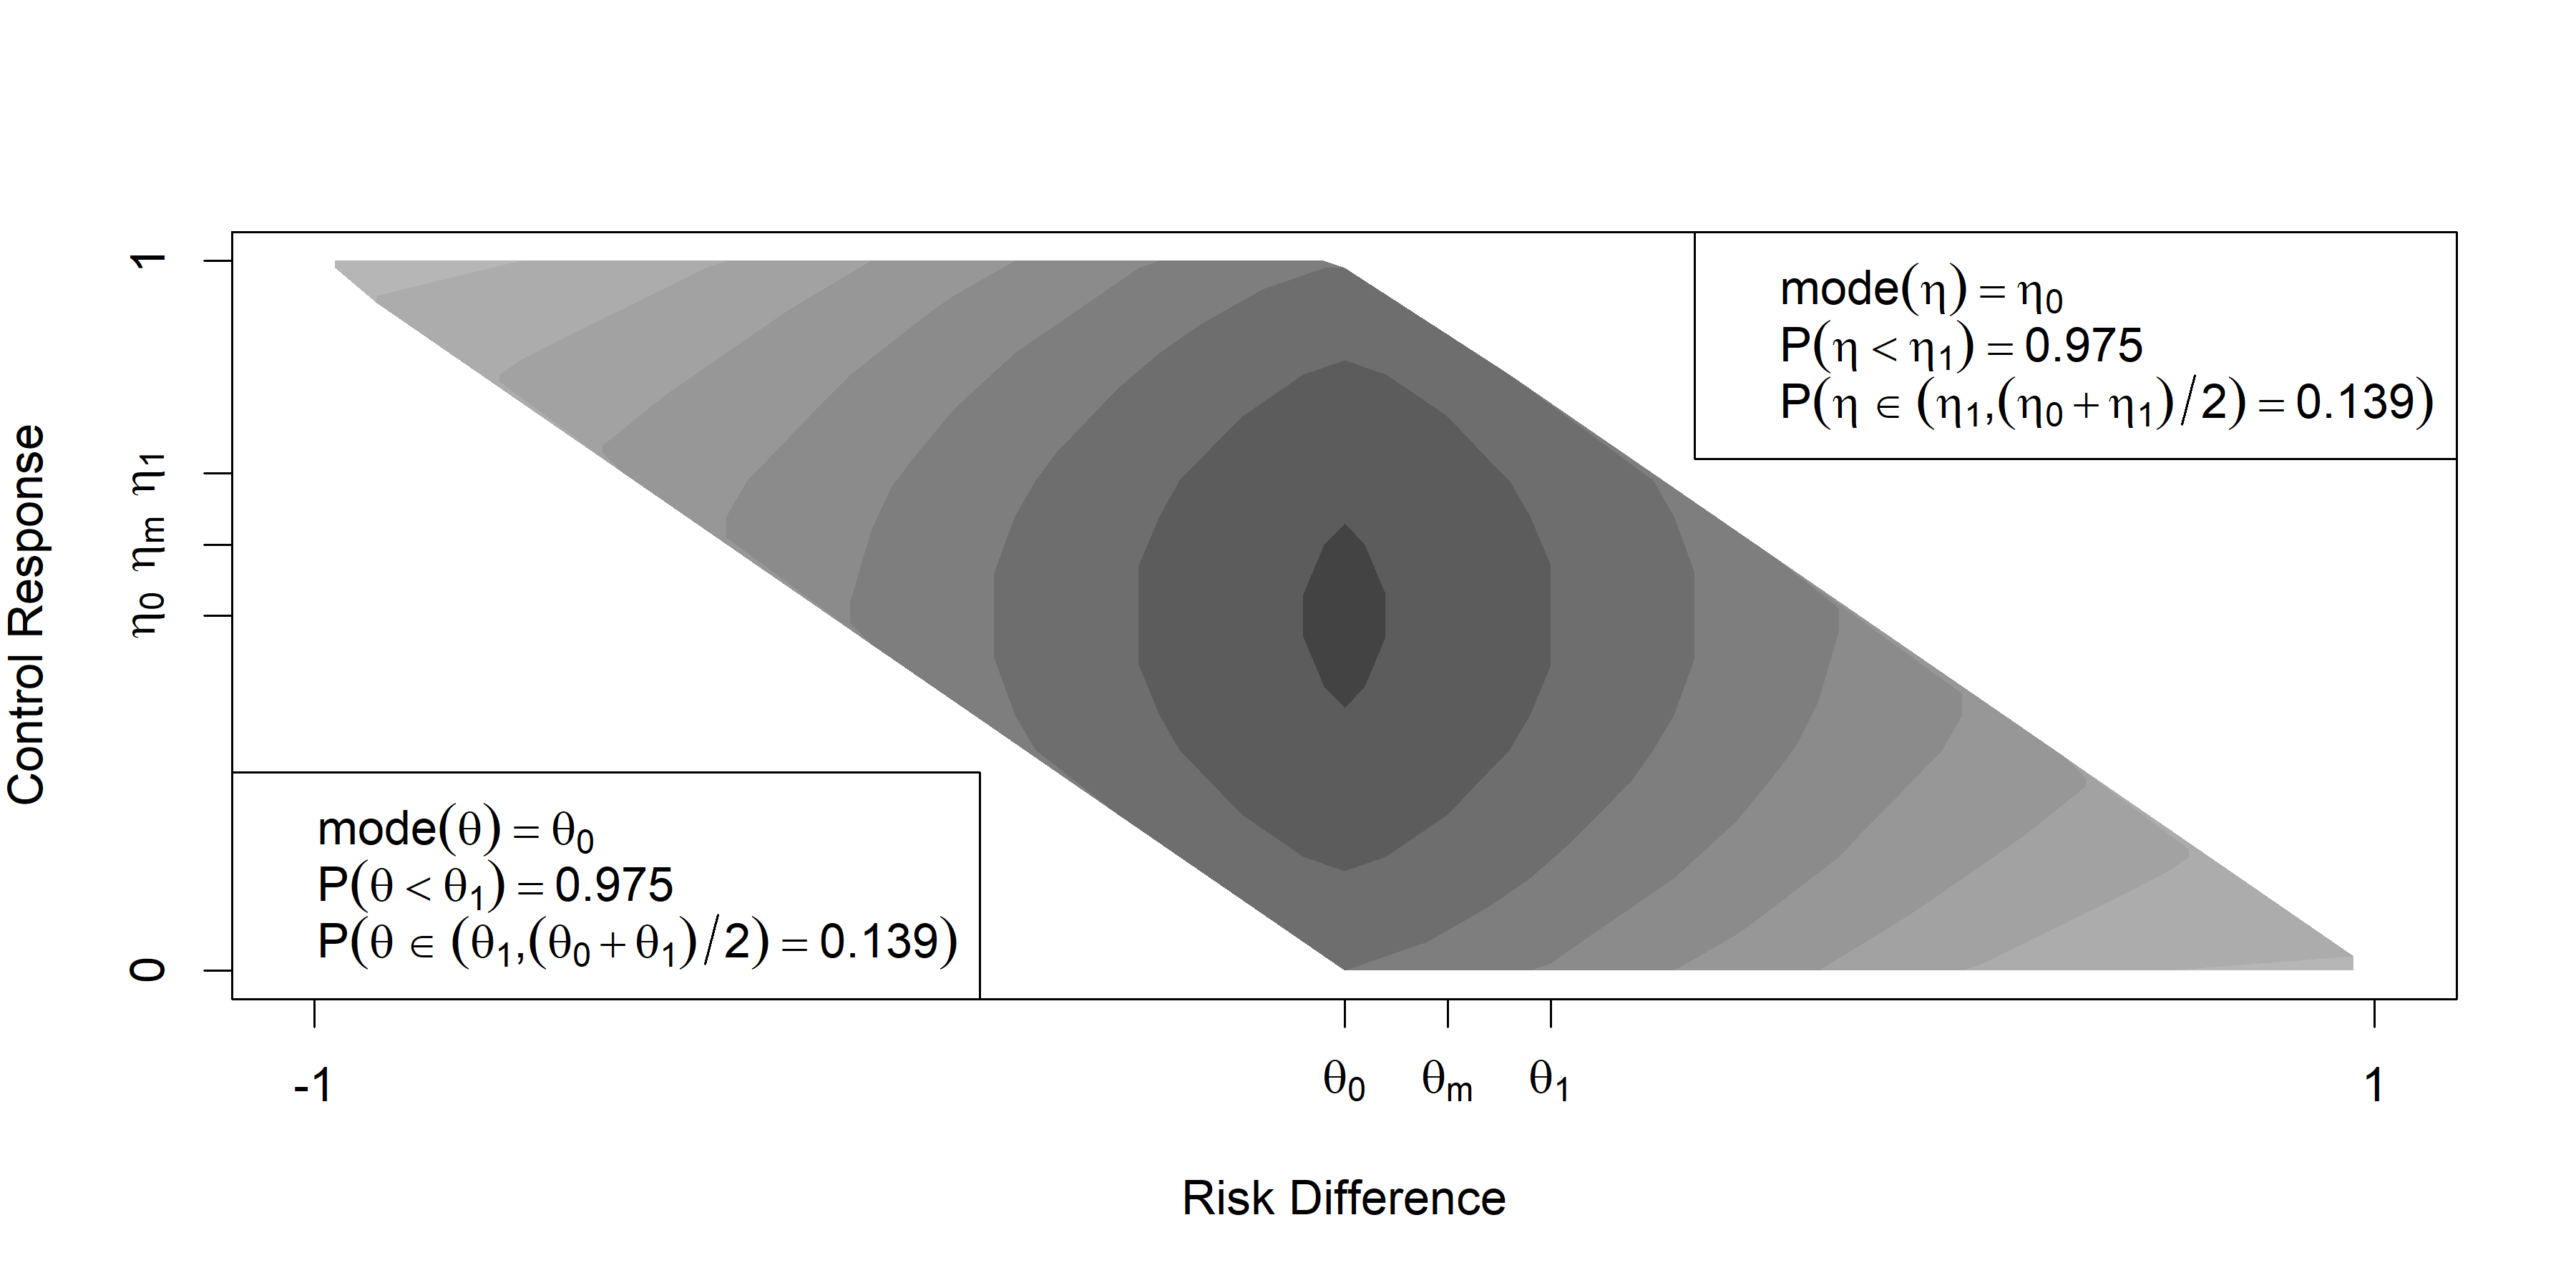
\includegraphics[width=6in]{figure5a.png}
%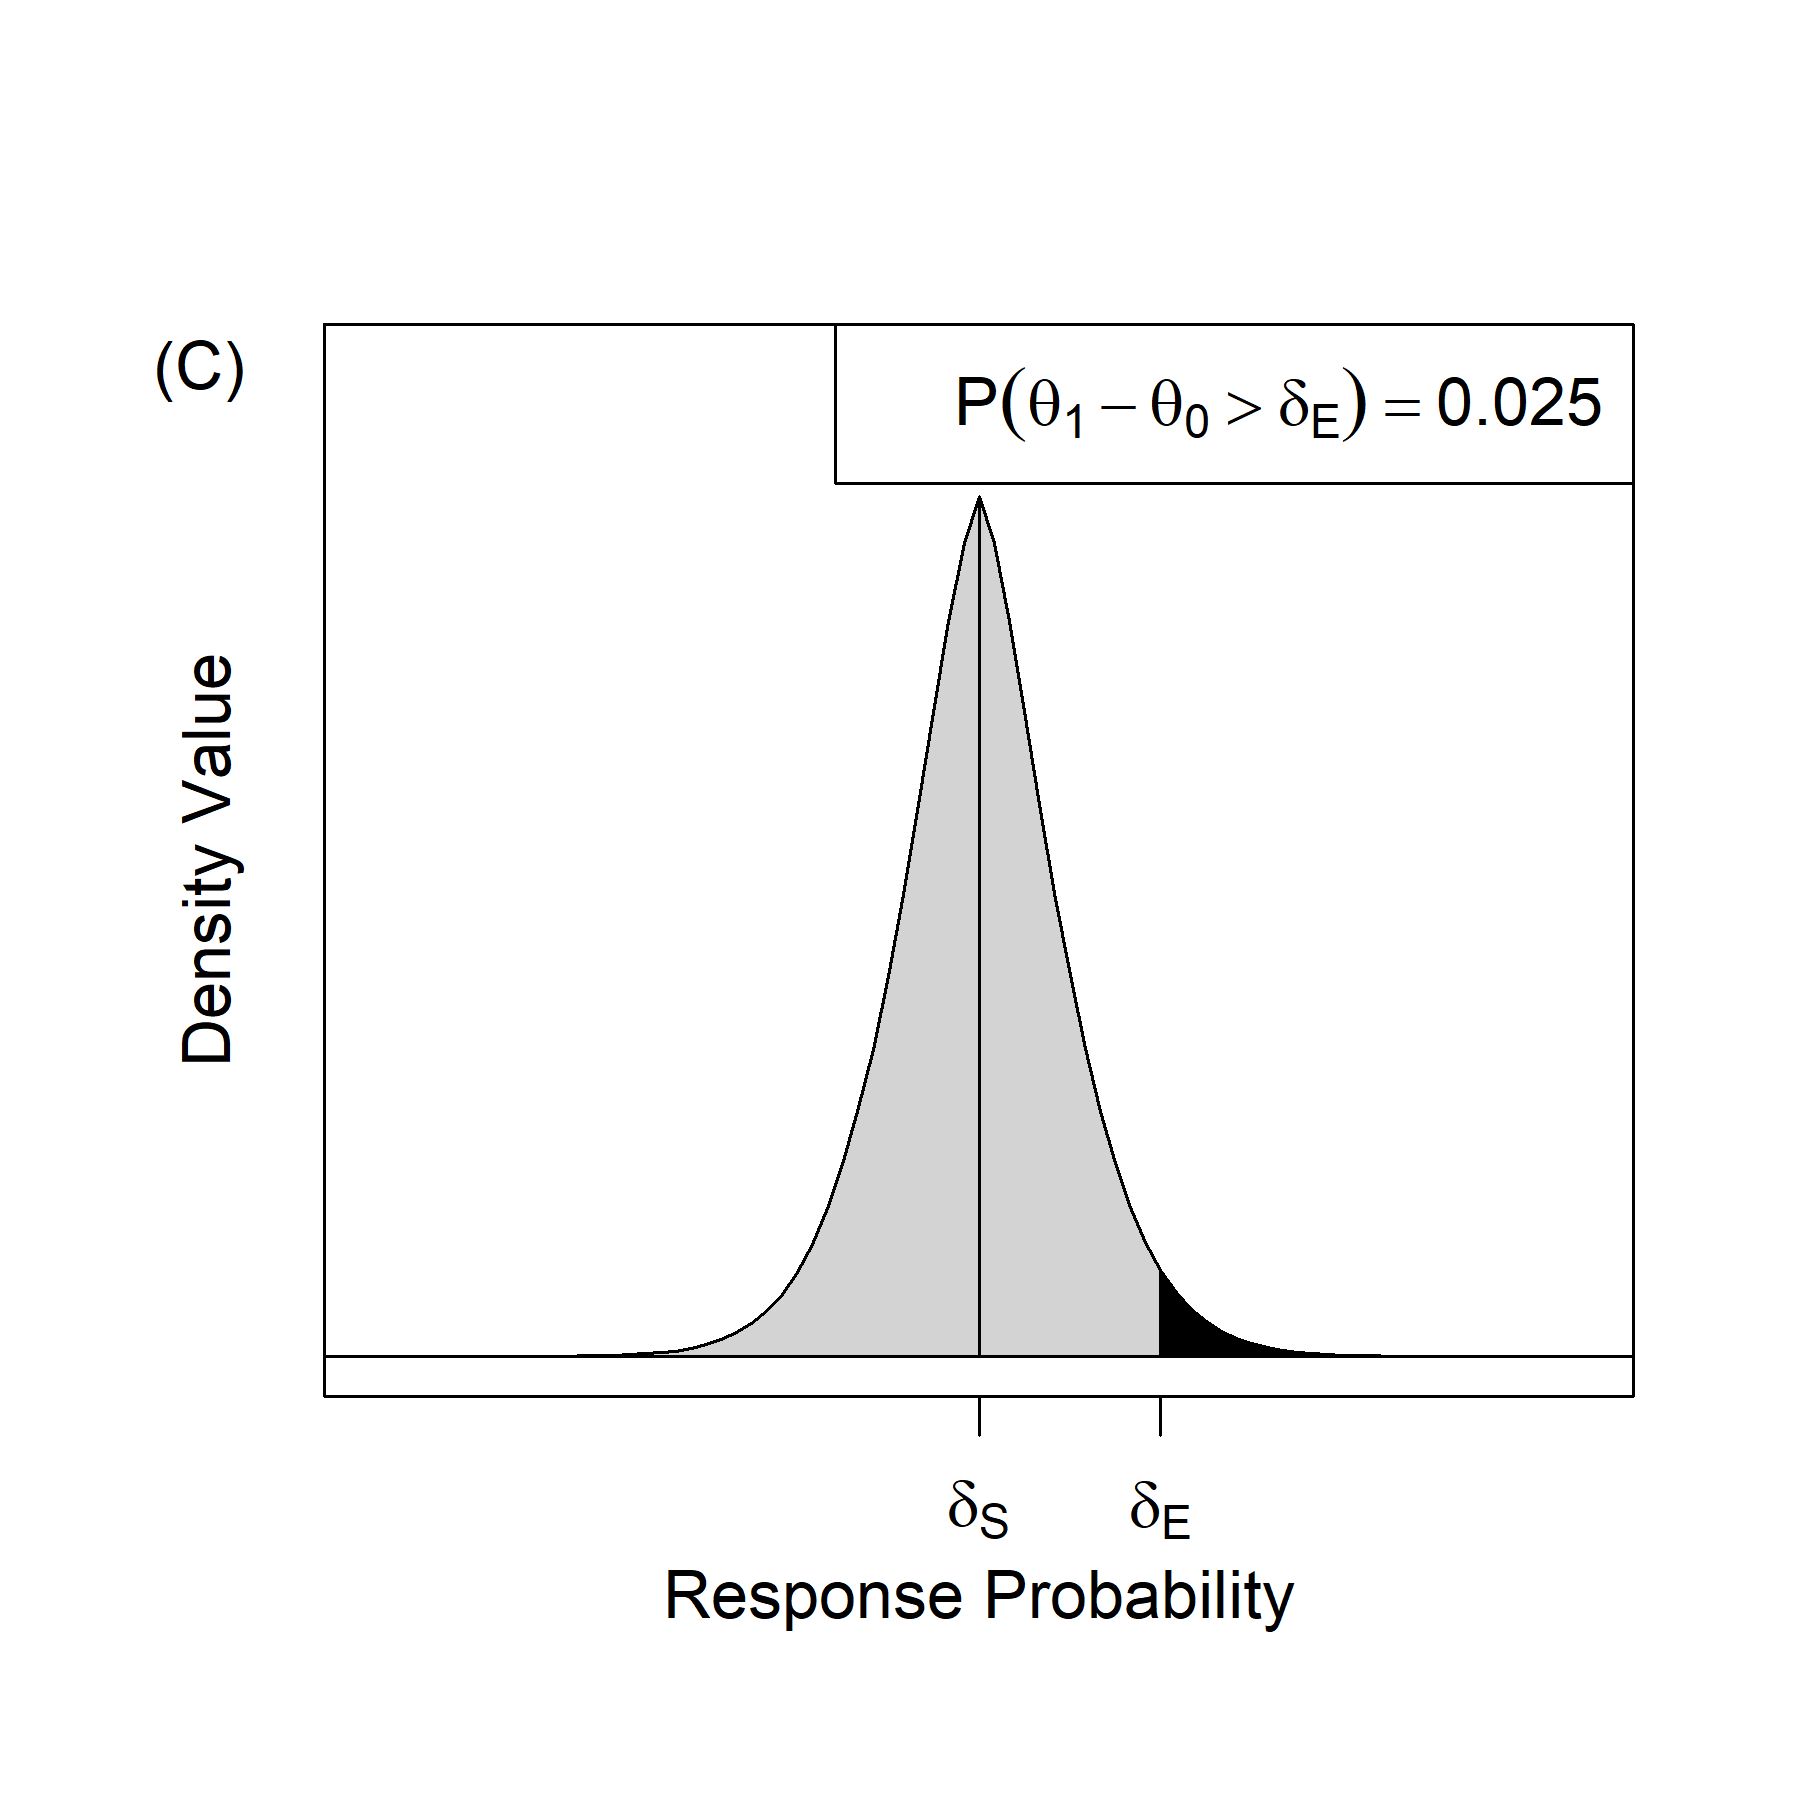
\includegraphics[width=6in]{figure5d.png}
%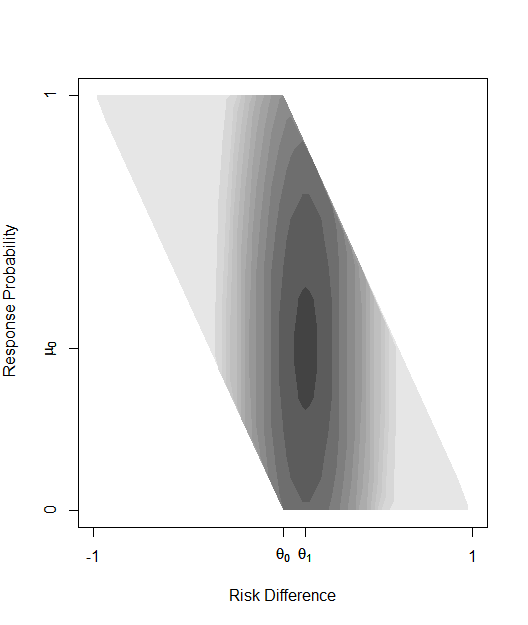
\includegraphics[width=6in]{figure5b.png}
%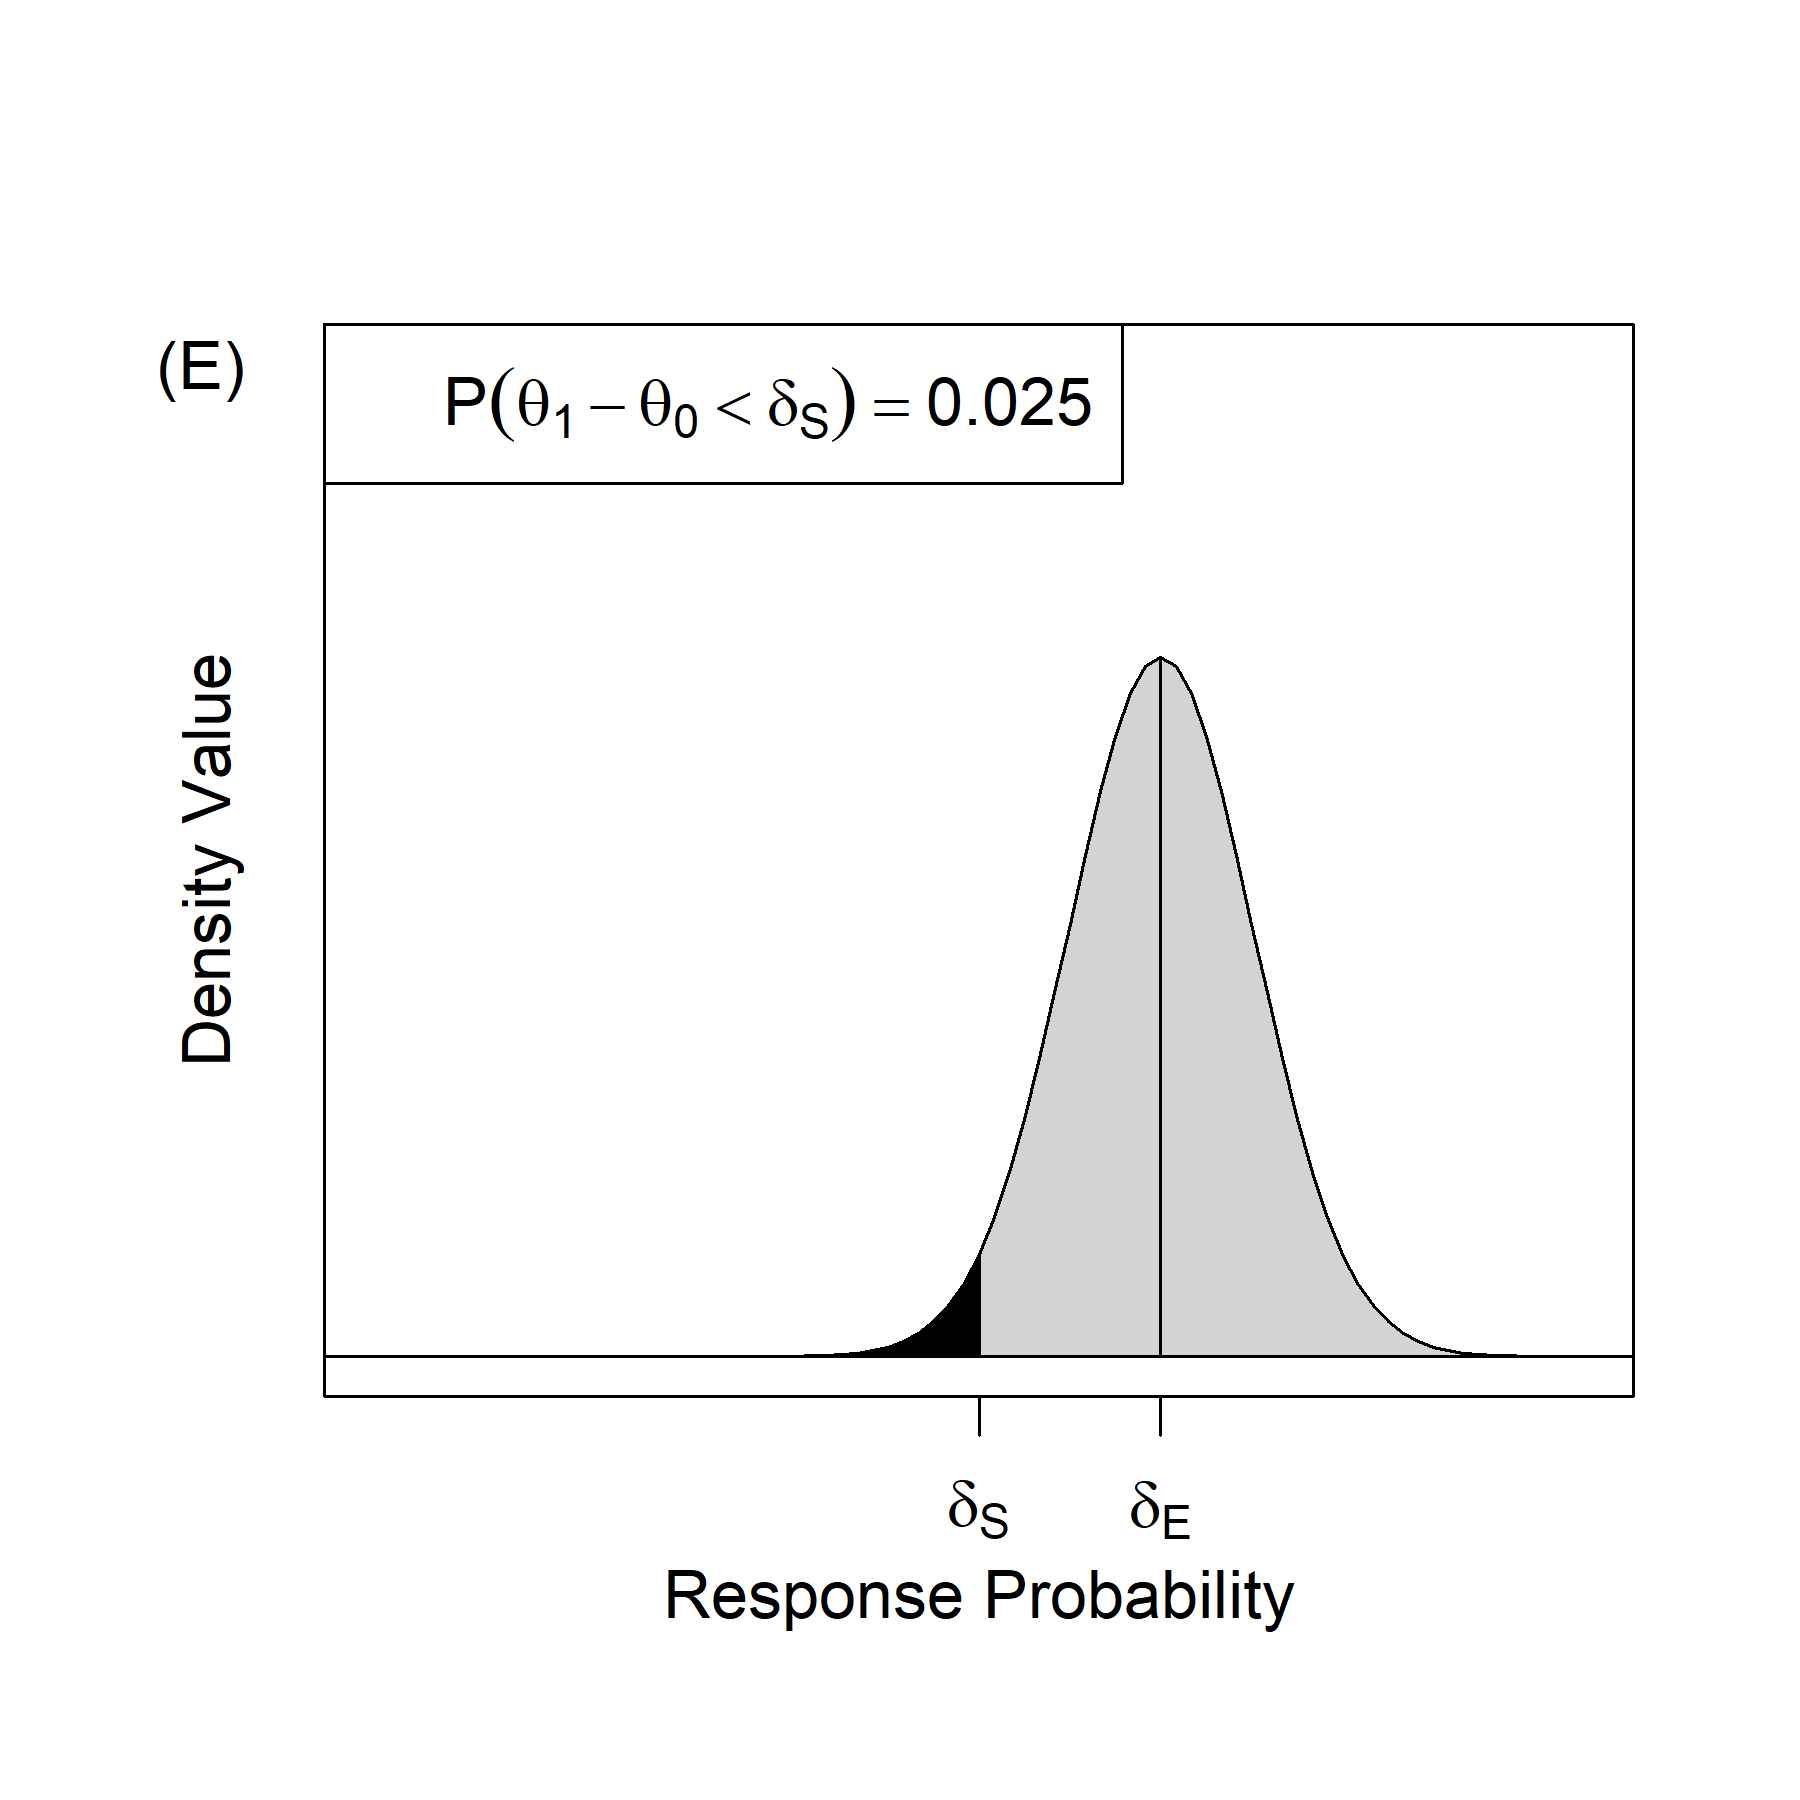
\includegraphics[width=6in]{figure5e.png}
\caption{A, Concentrated skeptical prior $\pi_S(\theta)$ truncated to $[-1,1]$. B, Conditional prior $\pi(\eta|\theta=\theta_0)$. C, Joint prior $\pi(\theta,\eta)=\pi(\theta)\times\pi(\eta|\theta)$ truncated based on the conditions $-1<\theta<1$ and $0<\theta+\eta<1$.}
\label{fig:figure5}
 \end{center}
\end{figure}

%\subsection{Operating Characteristics}
%\textcolor{red}{All of the concepts in this Section are basic and need not take up space in the main paper. I would cut this entire section. Still, I give some comments
%to help with clarity for the future (still, cut this all). There is some useful information in this section but it can be sprinkled in much more briefly when results are presented
%with notation revised according to the changes I made before. Keep the content of Section 2.3.4. Perhaps that can be a brief subsection of its own. The rest can go keeping on minimal discussion where the associated results are first presented.}

%\subsubsection{Expected sample size and trial duration}
%\textcolor{red}{I do not understand what this paragraph is saying. Neither the expected sample size or expected trial duration are rigorously defined. In the absence of that, 
%there is no point for this subsection.}
%Suppose that the trial has interim analyses based on the number of completed outcomes. Let $\bmath{D}(n)$ denote the data after $n$ completed outcomes are ascertained. Let $n_{\text{initial}}$ be the first instance where either the efficacy criteria \eqref{eq:efficacy_criteria} or futility criteria \eqref{eq:futility_criteria} are satisfied and enrollment is henceforth terminated, or $n_{\text{max}}$ if the efficacy criteria or futility criteria are not satisfied at any point. Let $n_{\text{final}}$ be the final sample size which includes patients whose outcomes were in progress at the time of enrollment termination. The expected trial duration is determined based the projected time needed for subject enrollment and outcome ascertainment for a number of subjects equal to the expected sample size.

%\subsubsection{Posterior mean and coverage probability}
%Any prior of the form \eqref{eq:inference_prior} and the data likelihood $\mathcal{L}(\theta|\mathbf{D})$ are used to evaluate the posterior distribution for $\theta$ denoted $\pi(\theta|\mathbf{D})$. The posterior mean at the final sample size is $E(\pi(\theta|\mathbf{D}(n_{\text{final}}))$. The coverage probability is the probability of the generating value of $\theta$ to be in an equal-tailed $100(1-\alpha)\%$ credible interval, which is the interval $[\theta^{(\alpha/2)},\theta^{(1-\alpha/2)}]$ based on the quantiles of the posterior distribution $\pi(\theta|\mathbf{D}(n_{\text{final}}))$.

%\subsubsection{Probability of efficacy, futility, and inconclusive findings}
%The probability of stopping early for efficacy and futility are the probability that the efficacy criteria \eqref{eq:efficacy_criteria} or futility criteria \eqref{eq:futility_criteria} are satisfied at an interim analysis with data $\mathbf{D}(n_{\text{initial}})$. The final determination of efficacy and futility refer to the corresponding criteria begin satisfied with data $\mathbf{D}(n_{\text{final}})$. To evaluate the frequentist properties of Bayesian designs, type I error and power are based on $\rmn{eff}(\bmath{D}(n_{\text{initial}}))$.  Inconclusive findings refers to situations where neither the efficacy or futility criteria are satisfied.

%\subsection{Design Considerations}
%\begin{enumerate}
%\item DC \#1
%\item DC \#2
%\item DC \#3
%\item DC \#4
%\item DC \#5
%\end{enumerate}

\section{Examples}\label{sec:examples}

\subsection{Single-Arm Proof-of-Activity Trial with Binary Endpoint}\label{sec:example1}
\subsubsection{Motivating Example}
We consider the T72 pediatric trial ``A Study of the Safety and Efficacy of Infliximab (REMICADE) in Pediatric Patients With Moderately to Severely Active Ulcerative Colitis" (NCT00336492) ~\citep{Hyams2012} which was conducted between August 2006 and June 2010.
%
The study population was patients ages 6 through 17 with moderate to sever ulcerative colitis defined as having a baseline Mayo score of 6 or above on a scale of 0-12, where higher scores indicate more severe disease activity.
%
A 5mg/kg dose of infliximab was given to patients at weeks 0, 2, and 6.
%
The primary endpoint was clinical response, corresponding to a 3-point or greater decrease in Mayo score from baseline to week 8. 
%
Patients were enrolled over approximately 33.5 months (approximately 1 patient enrolled per 17 days). 
%
The sample size of 60 patients was chosen so that a frequentist 95\% two-sided confidence interval for the response probability would have a half-width of 0.12 if the true response probability is 0.67.
%
The value 0.67 was the observed proportion of responders among adults with the same disease enrolled in the ACT 1 and ACT 2 trials \citep{Rutgeerts2005} who received the same weight-based dose of 5mg/kg (N = 242).
%
Obtaining a 95\% confidence interval that excluded 0.40 was used as the criterion for classifying the results as clinically significant.
%
Clinical response was observed in 44 of 60 (73.3\%) pediatric patients.

\subsubsection{Model Formulation \& Prior Elicitation}\label{sec:example1model} We use this trial as a motivating example to demonstrate the proposed 
framework for sequential monitoring. The data $\bmath{D}$ are assumed to be comprised of independent Bernoulli random variables having common response 
probability $\theta$. 
%
As mentioned above, the primary hypotheses evaluated in the trial were $H_0:\theta \le 0.4$ and $H_1: \theta>0.4$.
%
For purposes of monitoring, we took $\theta_1=0.67$ consistent with the ACT 1 and ACT 2 trial data. 
%
The example presented in this section make use of a concentrated skeptical prior and a default enthusiastic prior for monitoring.
%
%\textcolor{red}{Make sure this is moved to supplemental appendix and appropriately referenced. See my recent paper in biometrics for examples for how to write references to the online supplementary materials.}
%
A comparison of design properties based on various combinations of the monitoring priors is given in Web Appendix D.
%
In this example, we considered an inference prior defined as the mixture \eqref{eq:3partmix} using the values $\omega_S=\omega_E=0.5$ (i.e., a non-adaptive inference prior), which was used to determine the posterior mean and 95\% credible intervals. For sequential monitoring, we consider analyzing the accumulating data after every two patients complete follow-up.

The early stopping criteria, as well as any quantity involving the posterior distribution of $\theta$ requires evaluating integrals of the dimension of $\theta$ (or the dimension of $(\theta,\eta)$ in the case of nuisance parameters).
%
For the cases we consider in this paper, these quantities are 1$-$ or 2$-$dimensional integrals which are evaluated using numerical integration in R \citep{R2017} using the \texttt{pracma} package \citep{Borchers2019}.

\subsubsection{Example Paths}
Figure 3 presents violin plots to illustrate the monitoring process for two hypothetical instances of the trial. 
%
For each instance, the monitoring priors (left-most set of distributions), and the posterior distributions at three selected interim analyses (middle sets) and from the final analysis (right-most set) are shown.
	%
Panel A of Figure \ref{fig:figure2} shows the results of a trial with early stopping for efficacy once 30 outcomes are ascertained, and enrollment is henceforth terminated. 
%
The final data (i.e., the data after ongoing patients are followed-up) in this example no longer meet the criteria for a compelling demonstration of efficacy.
	%
%A discussion of this type of evidence attenuation is given in Section \ref{sec:evid_decrease}.
%
Panel B of Figure \ref{fig:figure2} shows the results of a trial with early stopping for futility once 30 outcomes are ascertained, and enrollment is henceforth terminated. The final data matches the last interim analysis since enrolled patients would be transitioned off the IP.

\begin{figure}\begin{center}
    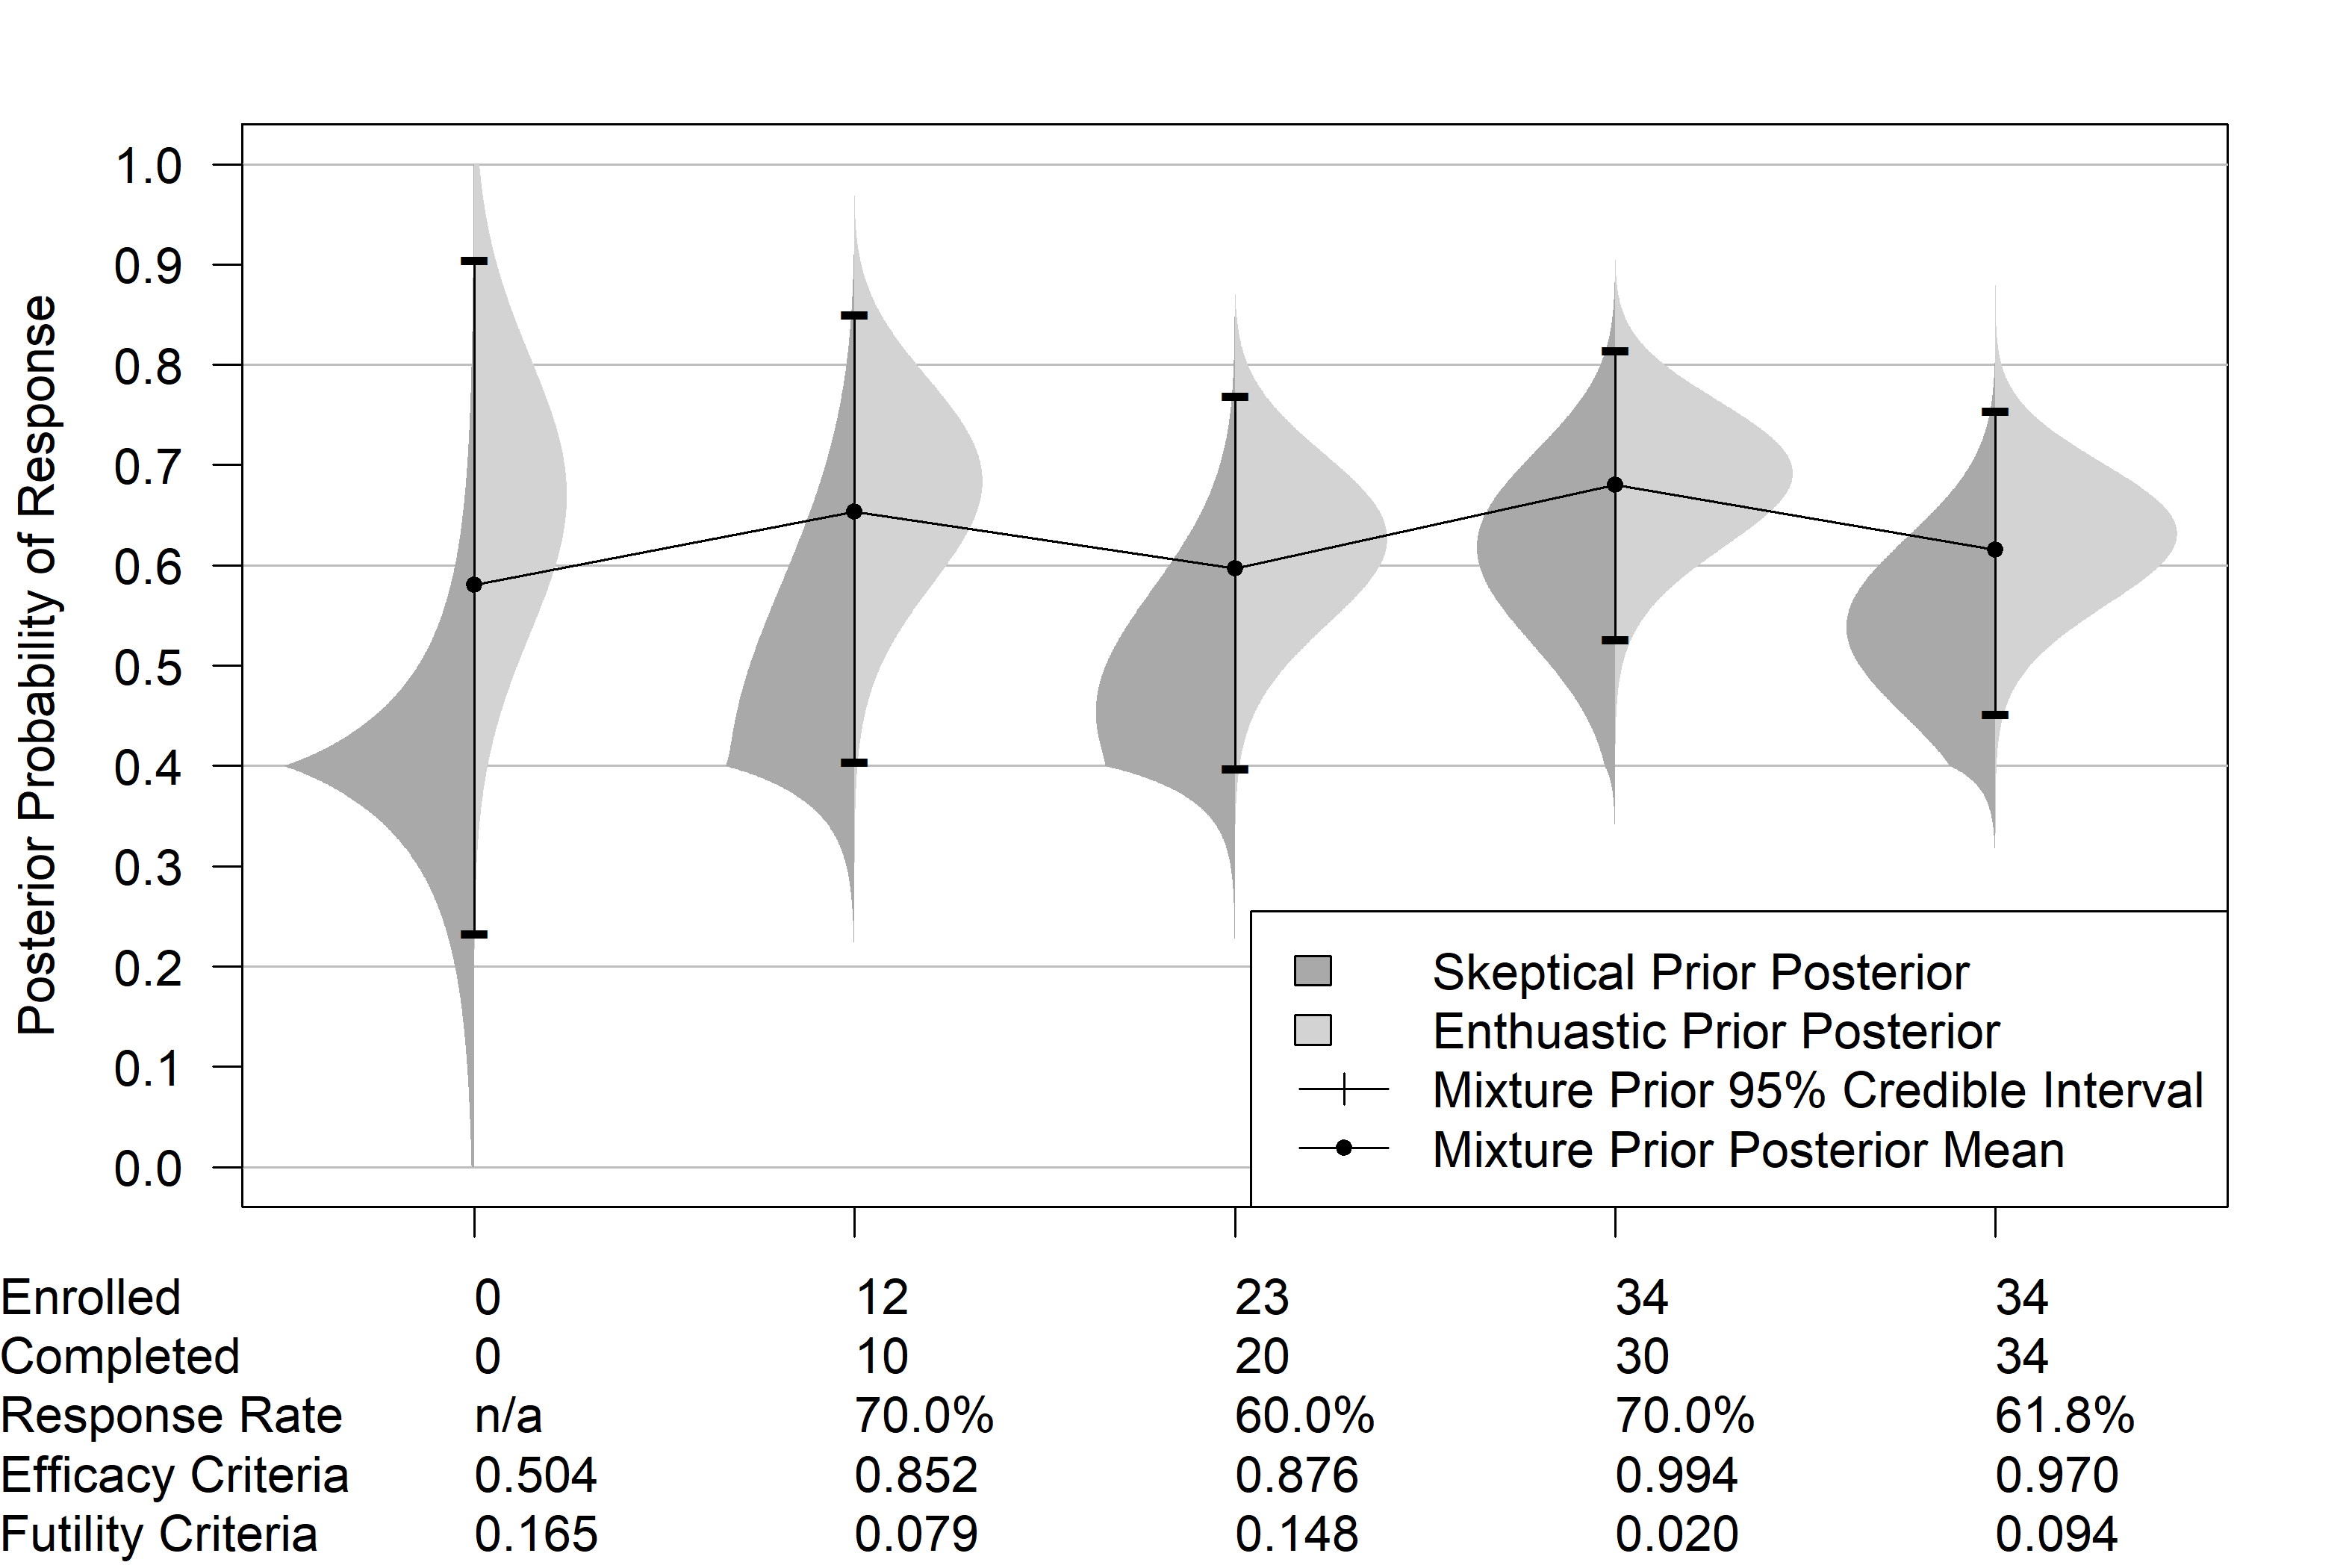
\includegraphics[width=6in]{figure2a.png}
    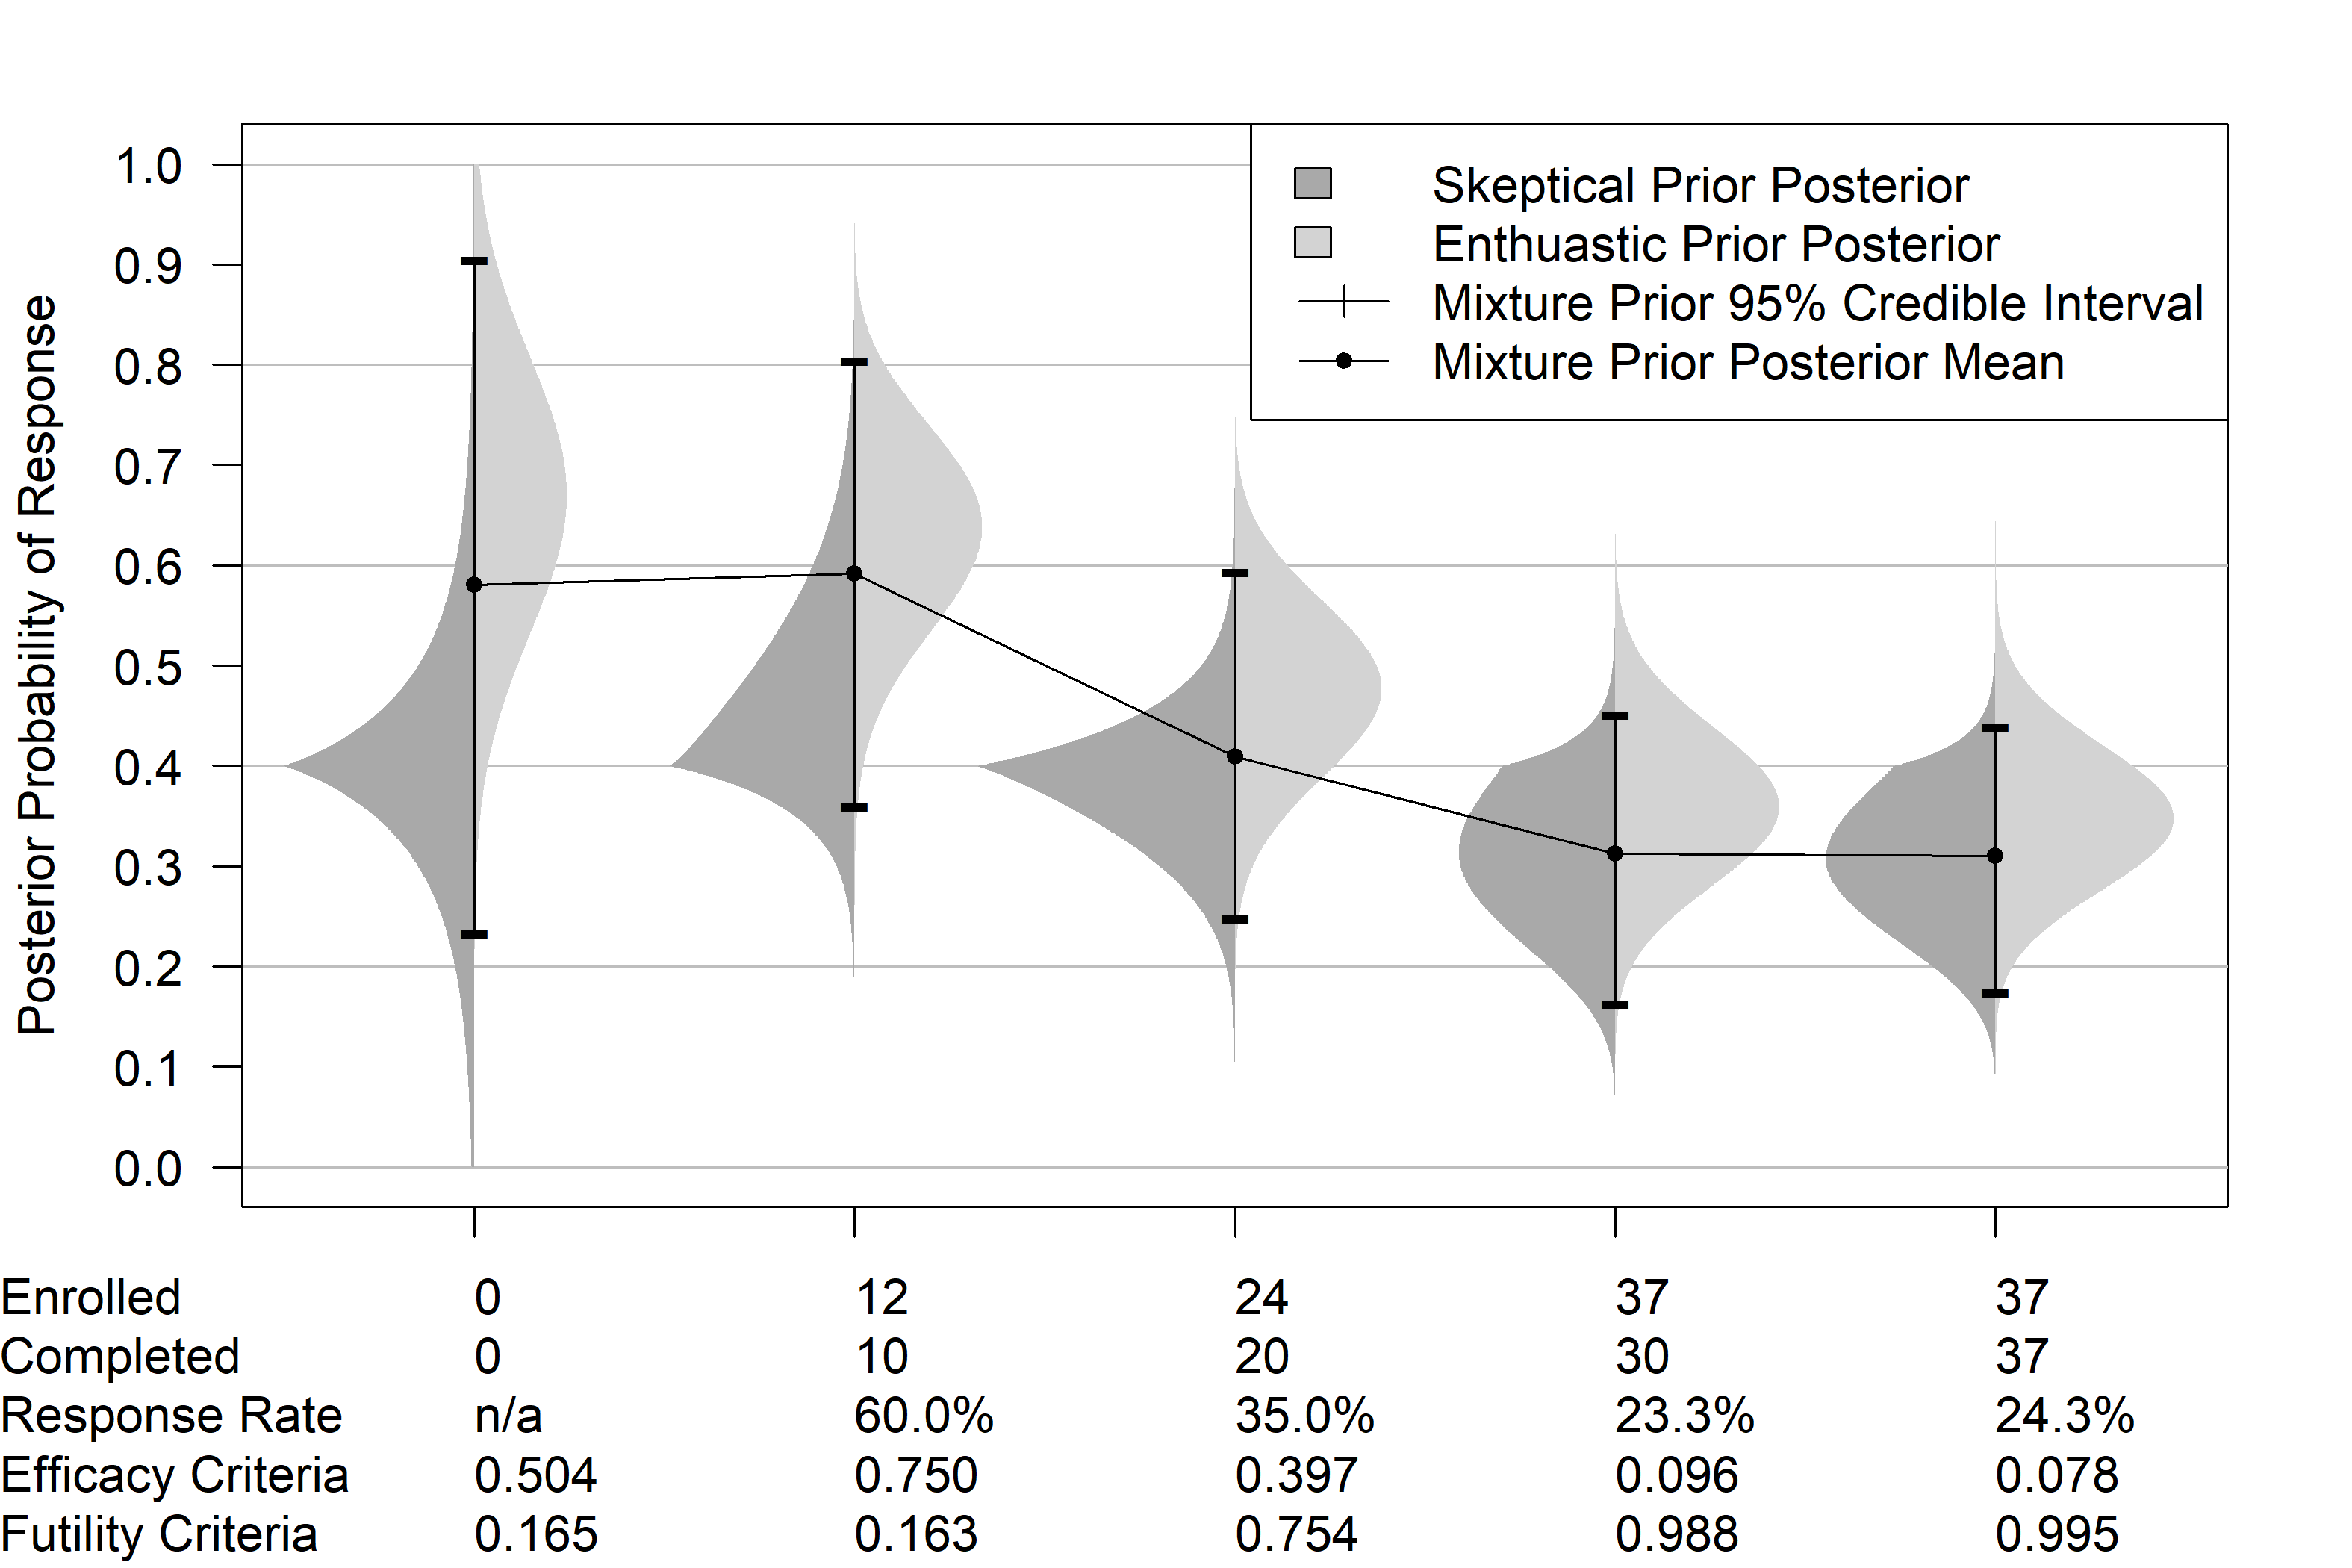
\includegraphics[width=6in]{figure2b.png}
    \caption{Example paths for the trial described in Section \ref{sec:example1model}. A, Early stoppage for efficacy. B, Early stoppage for futility.}
	\label{fig:figure2}
\end{center}
\end{figure}

\subsubsection{Preposterior Analysis of Operating Characteristics}\label{sec:ex1.1}
The operating characteristics presented in this section are estimated using $100,000$ simulated trials per value of $\theta$ using the trial design as described in Section \ref{sec:example1model}. 
%
As shown in Panel A of Figure \ref{fig:ex1.1}, when the true response probability is $\theta_0=0.4$, the probability of stopping the trial early for efficacy is equal to $0.026$, and at $\theta_1=0.67$ it is $0.953$. 
%
% The expected sample size is less than 60 for each value of $\theta$ considered. 
Interim stoppage for either efficacy or futility occurred in each simulation (i.e., the maximum sample size was such that the trial could not reach the maximum). The expected sample sizes are the lowest when the true response probabilities are $\theta_0$ or $\theta_1$. This is because the trial is more likely to be stopped for futility or efficacy when the data are consistent with the skeptical or enthusiastic priors respectively, which have modes at $\theta_0$ and $\theta_1$. 
%
At $\theta_0=0.4$, the posterior mean estimates using the mixture prior are slightly greater than the true underlying value, and at $\theta_1=0.67$, the posterior estimates using the mixture prior are slightly less than the true underlying value. 
%
This slight bias towards the interval $[\theta_0,\theta_1]$ is because those are the values determined to be the most likely a priori by the mixture prior.
% This is because the mixture prior is a weighted combination of priors that have $\theta_0$ and $\theta_1$ as the most likely values, and the enthusiastic component with mode $\theta_1$ contributes bias towards greater values. 
%
% In a similar way, at $\theta_1=0.67$, the posterior estimates using the mixture prior are slightly less than the true underlying value because the skeptical component with mode $\theta_0$ contributes bias towards smaller values. 
%
The 95\% credible intervals are shown to have coverage probabilities exceeding their nominal level for all values of $\theta$ considered.
%
%For the generating values of $\theta$ considered, the posterior mean shows bias towards the alternative hypothesis.
%%
%This is because the inference prior is still informative towards to alternative hypothesis.
%%
%The coverage probability of an equal-tailed $95\%$ credible interval is shown to cover the true generating value of $\theta$ with more than $95\%$ probability when $\theta$ is near $\theta_0$ or $\theta_1$, and less than $95\%$ of the time when $\theta$ is an intermediate value (e.g. final coverage probability of $93.1\%$ when $\theta=0.535$.
%%
%This is because the mixture prior places high prior probability near $\theta_0$ and $\theta_1$ and less prior probability at intermediate values.

Given that the early stopping criteria was satisfied as an interim analysis, it is of interest to compare the posterior probability of the alternative once patients in follow-up have completed outcomes using the same skeptical prior.
%
It is of particular interest when the threshold for a compelling demonstration is satisfied for an interim analysis but is no longer satisfied once outcomes from patients in progress are ascertained, as was the case in Panel A of Figure \ref{fig:figure2}.
%
The probability of such an occurrence and the difference between the posterior probabilities evaluated at the different time points is shown in Panel B of Figure \ref{fig:ex1.1}.
%
The probability of these cases occurring is reflected by the percent agreement between interim and final results.
%
Recall that when the generating value of theta is $\theta_0=0.4$, the trial is stopped early for efficacy with probability $0.026$. Among these cases, the posterior probability is still greater than $1-\epsilon$ with probability $0.433$. 
%
This means that the completed outcomes from patients in progress at time enrollment was terminated are likely to meaningfully diminish the evidence in favor of efficacy relative to the threshold for what is viewed as compelling.
%
When the generating value of theta is $\theta_1=0.67$, the trial is stopped early for efficacy with probability $0.952$, and among those cases the posterior probability is  greater than $1-\epsilon$ with probability $0.887$.

The distribution of the posterior probability given the final data for these cases demonstrate that even in the cases where there is evidence decrease, the final posterior probability is still similar to the $1-\epsilon=0.975$ threshold.
%
Consider $\theta_1=0.67$: in the $11.3\%$ of situations where there is evidence decrease below the $1-\epsilon=0.975$ threshold, $90\%$ of these cases have a final posterior probability of approximately $0.93$ or greater. 
%
These analyses show that even if the skeptical prior was used for the final determination of efficacy rather than an inference prior, the final posterior probability of the alternative would be similar to that which triggered stoppage of enrollment, and the level of similarity increases as the underlying response probability $\theta$ increases.
%

\begin{figure}\begin{center}

    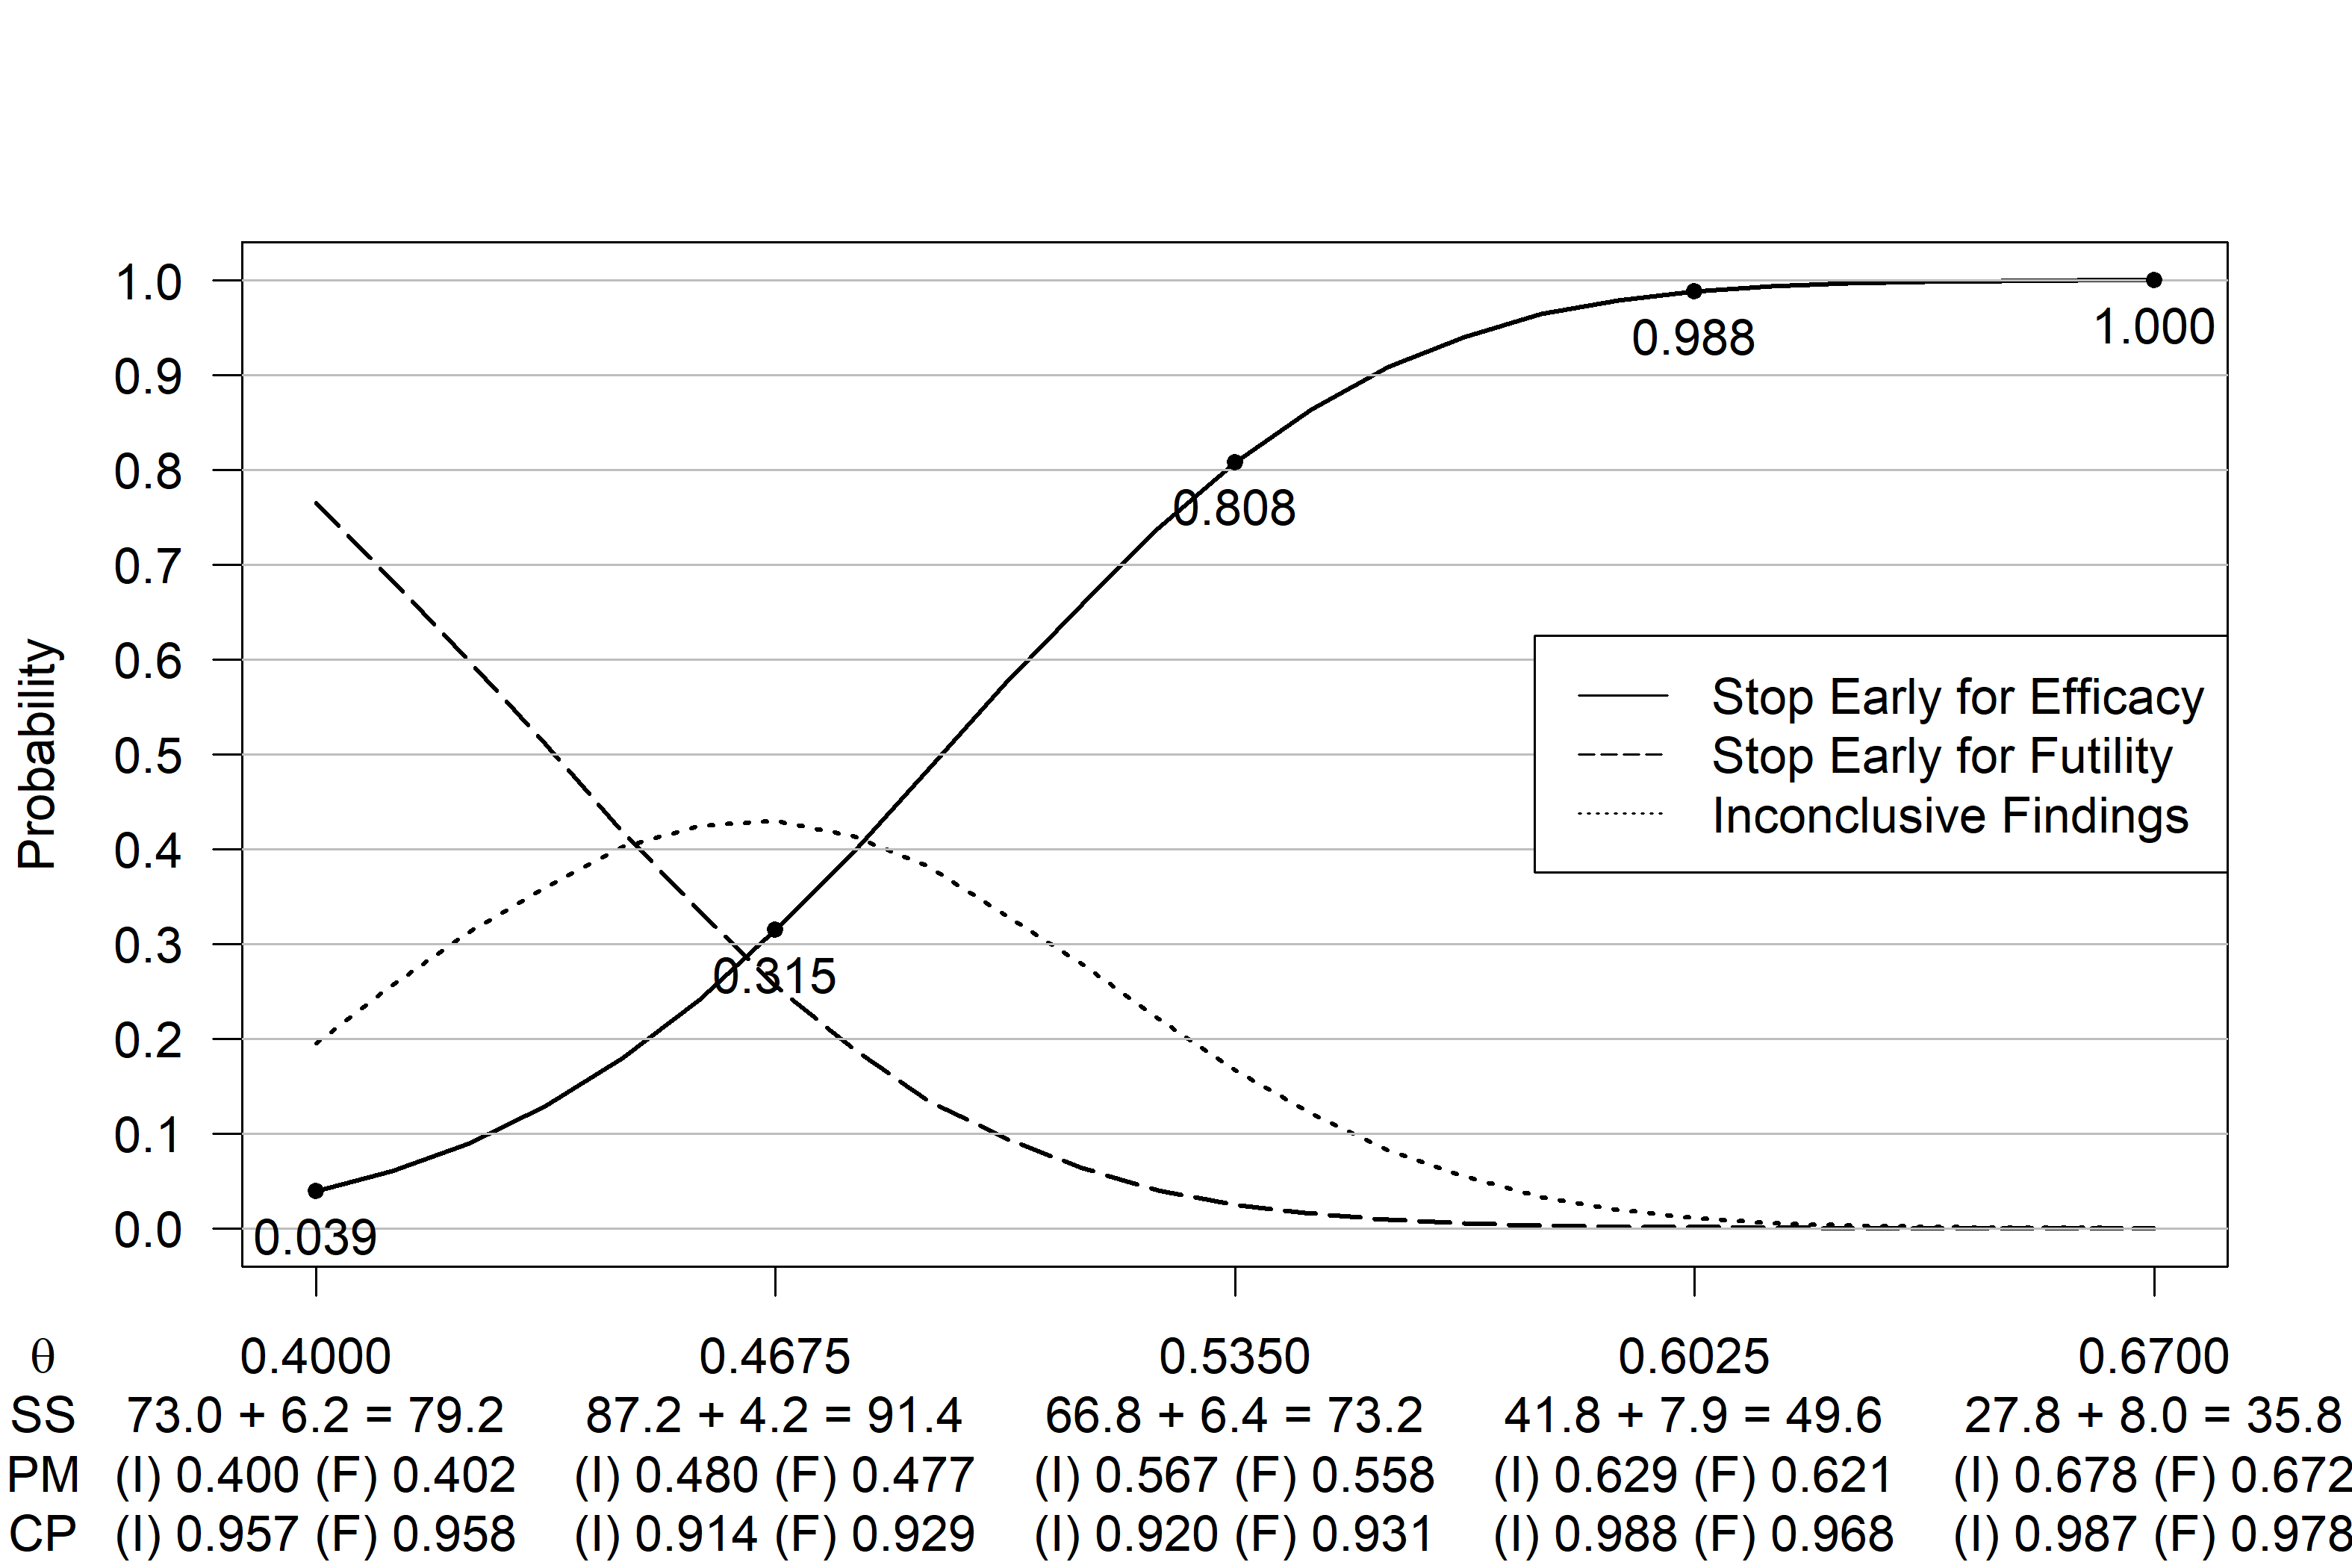
\includegraphics[width=6in]{figure3a.png}
    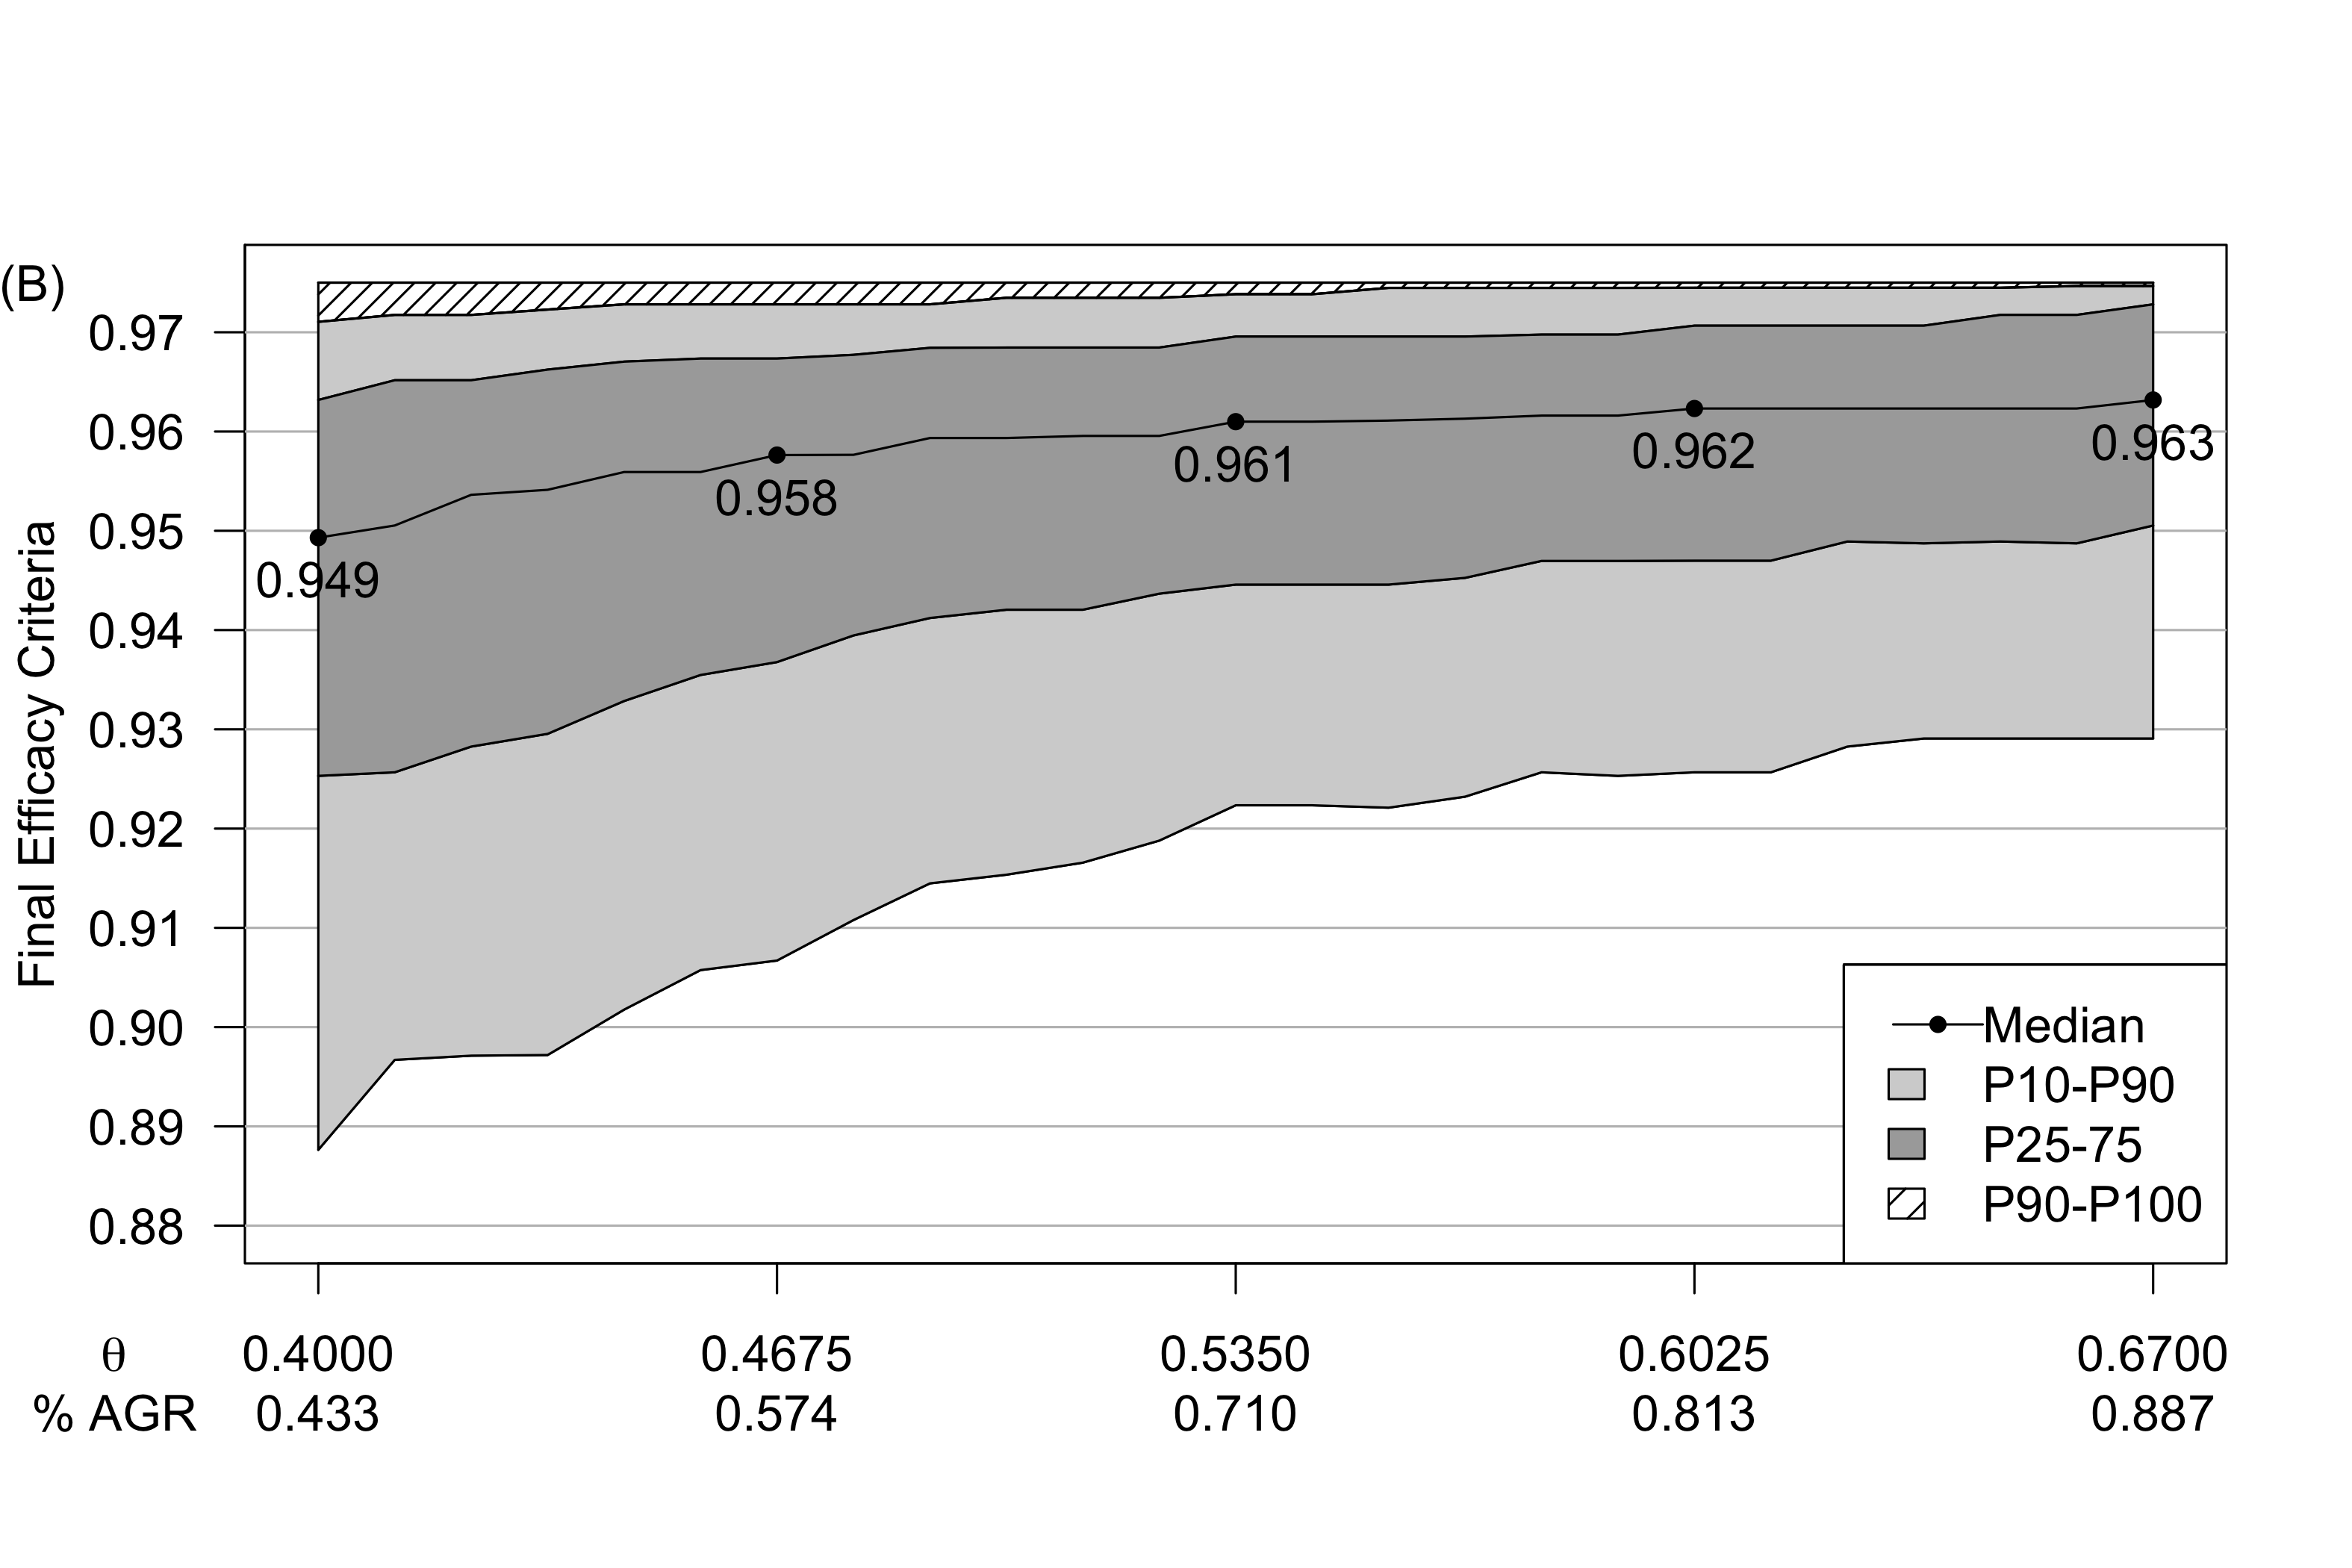
\includegraphics[width=6in]{figure3b.png}
    \caption{A, Sequential design properties. (SS; mean sample size, PM; posterior mean, CP; coverage probability, (I); interim analysis, (F); final analysis). B, Distribution of final posterior probability given interim stoppage and evidence decrease ($\%$ AGR; percent of agreement between final and interim posterior probabilities relative to $1-\epsilon$ threshold).}
	\label{fig:ex1.1}

\end{center}
\end{figure}
\subsubsection{Type 1 Error Rate by the Frequency of Data Monitoring}\label{sec:ex1t1e}
Figure \ref{fig:ex1t1e} shows the probability of stopping early for efficacy and the posterior probability that the alternative hypothesis is true at the final analysis assuming true response probability of $\theta_0=0.4$. 
%
The monitoring frequency is one when an interim analysis is made after every completed outcome (i.e. fully sequential), and is 60 (the maximum sample size) if the only analysis is done at the maximum sample size.
%
When there is only a single analysis completed at the maximum sample size, the probability of determining efficacy with the skeptical monitoring prior is $1.3\%$.
%
%This is because the determination of efficacy is made with an informative skeptical prior.
%
%If the determination of efficacy was made with a non-informative prior, then the probability of the efficacy criteria being satisfied with a single analysis completed at the maximum sample size would be $2.5\%$.
%
For more frequent data monitoring, the probability of obtaining a compelling demonstration of efficacy at an interim analysis increases slightly, but never far exceeds the typical nominal level. 
%
In many of these cases with early stoppage for efficacy with a true $\theta=\theta_0$, the final posterior probability which includes the total follow-up no longer meets the threshold for a compelling demonstration.
\begin{figure}\begin{center}

    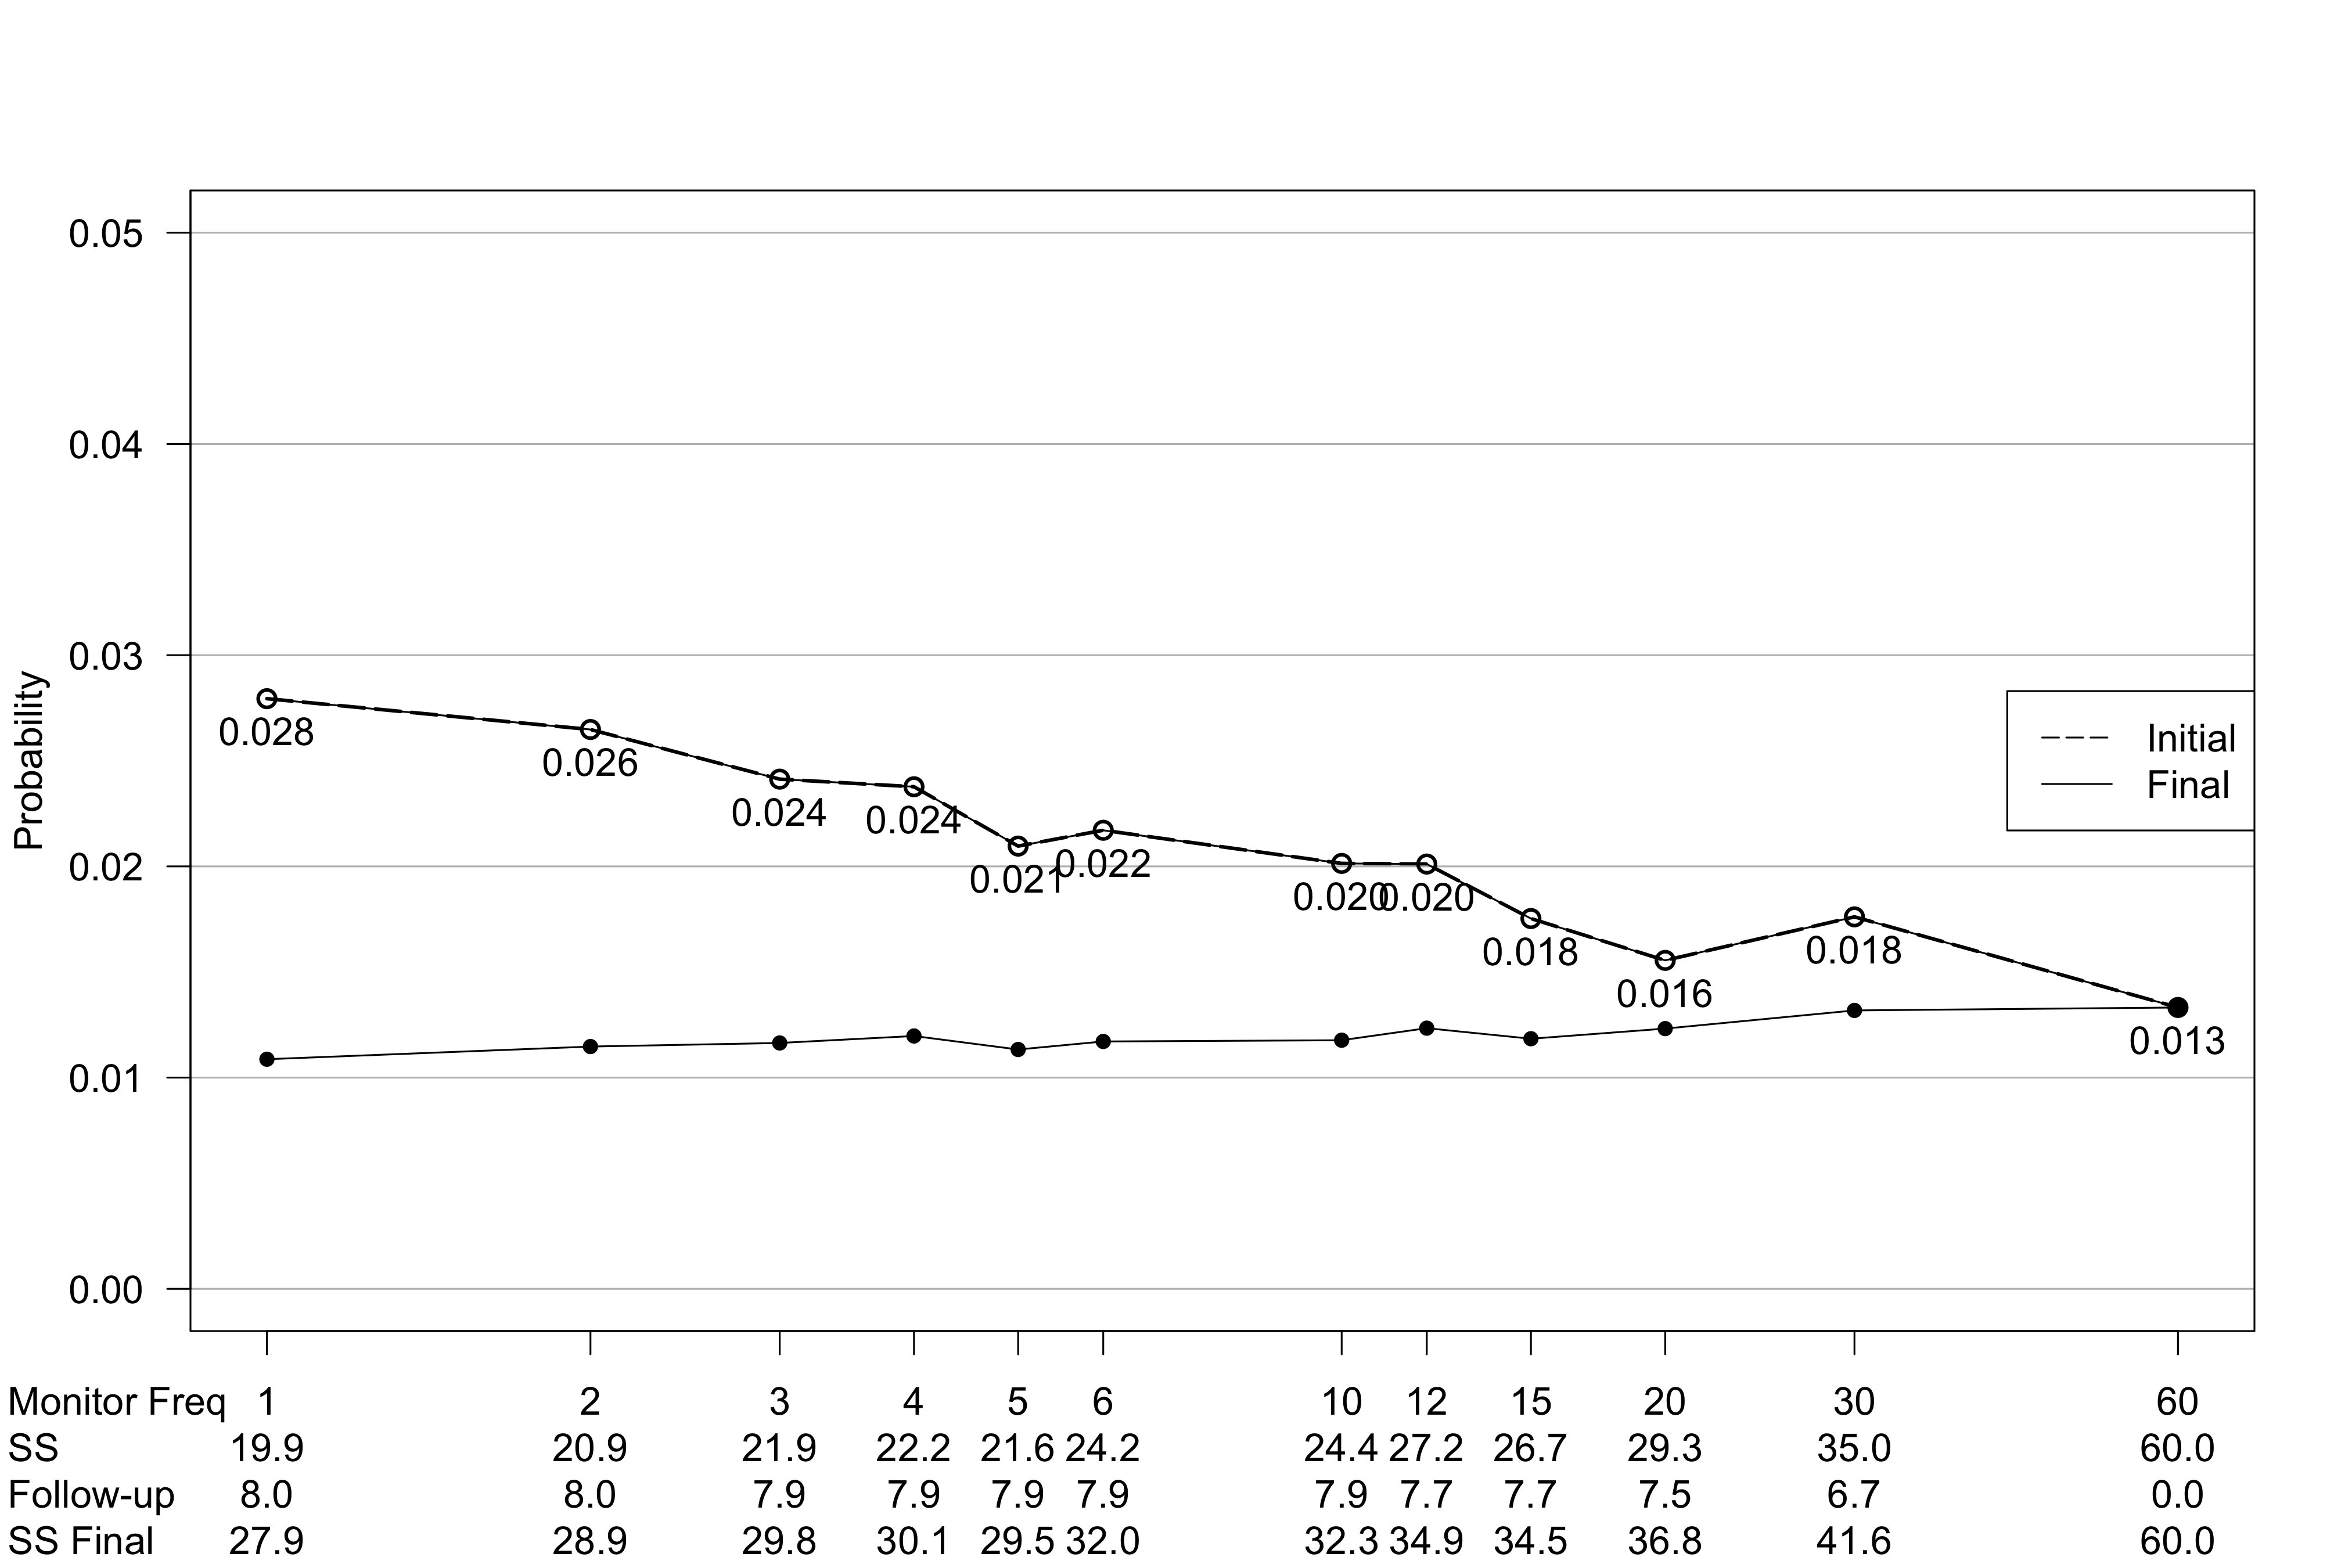
\includegraphics[width=6in]{figure4.png}
    \caption{Probability of stopping early for efficacy and the posterior probability that the alternative hypothesis is true at the final analysis when $\theta=\theta_0$ (SS; mean sample size, Monitor Freq; monitoring frequency).}
	\label{fig:ex1t1e}

%  \begin{subfigure}{7in}
%    \centering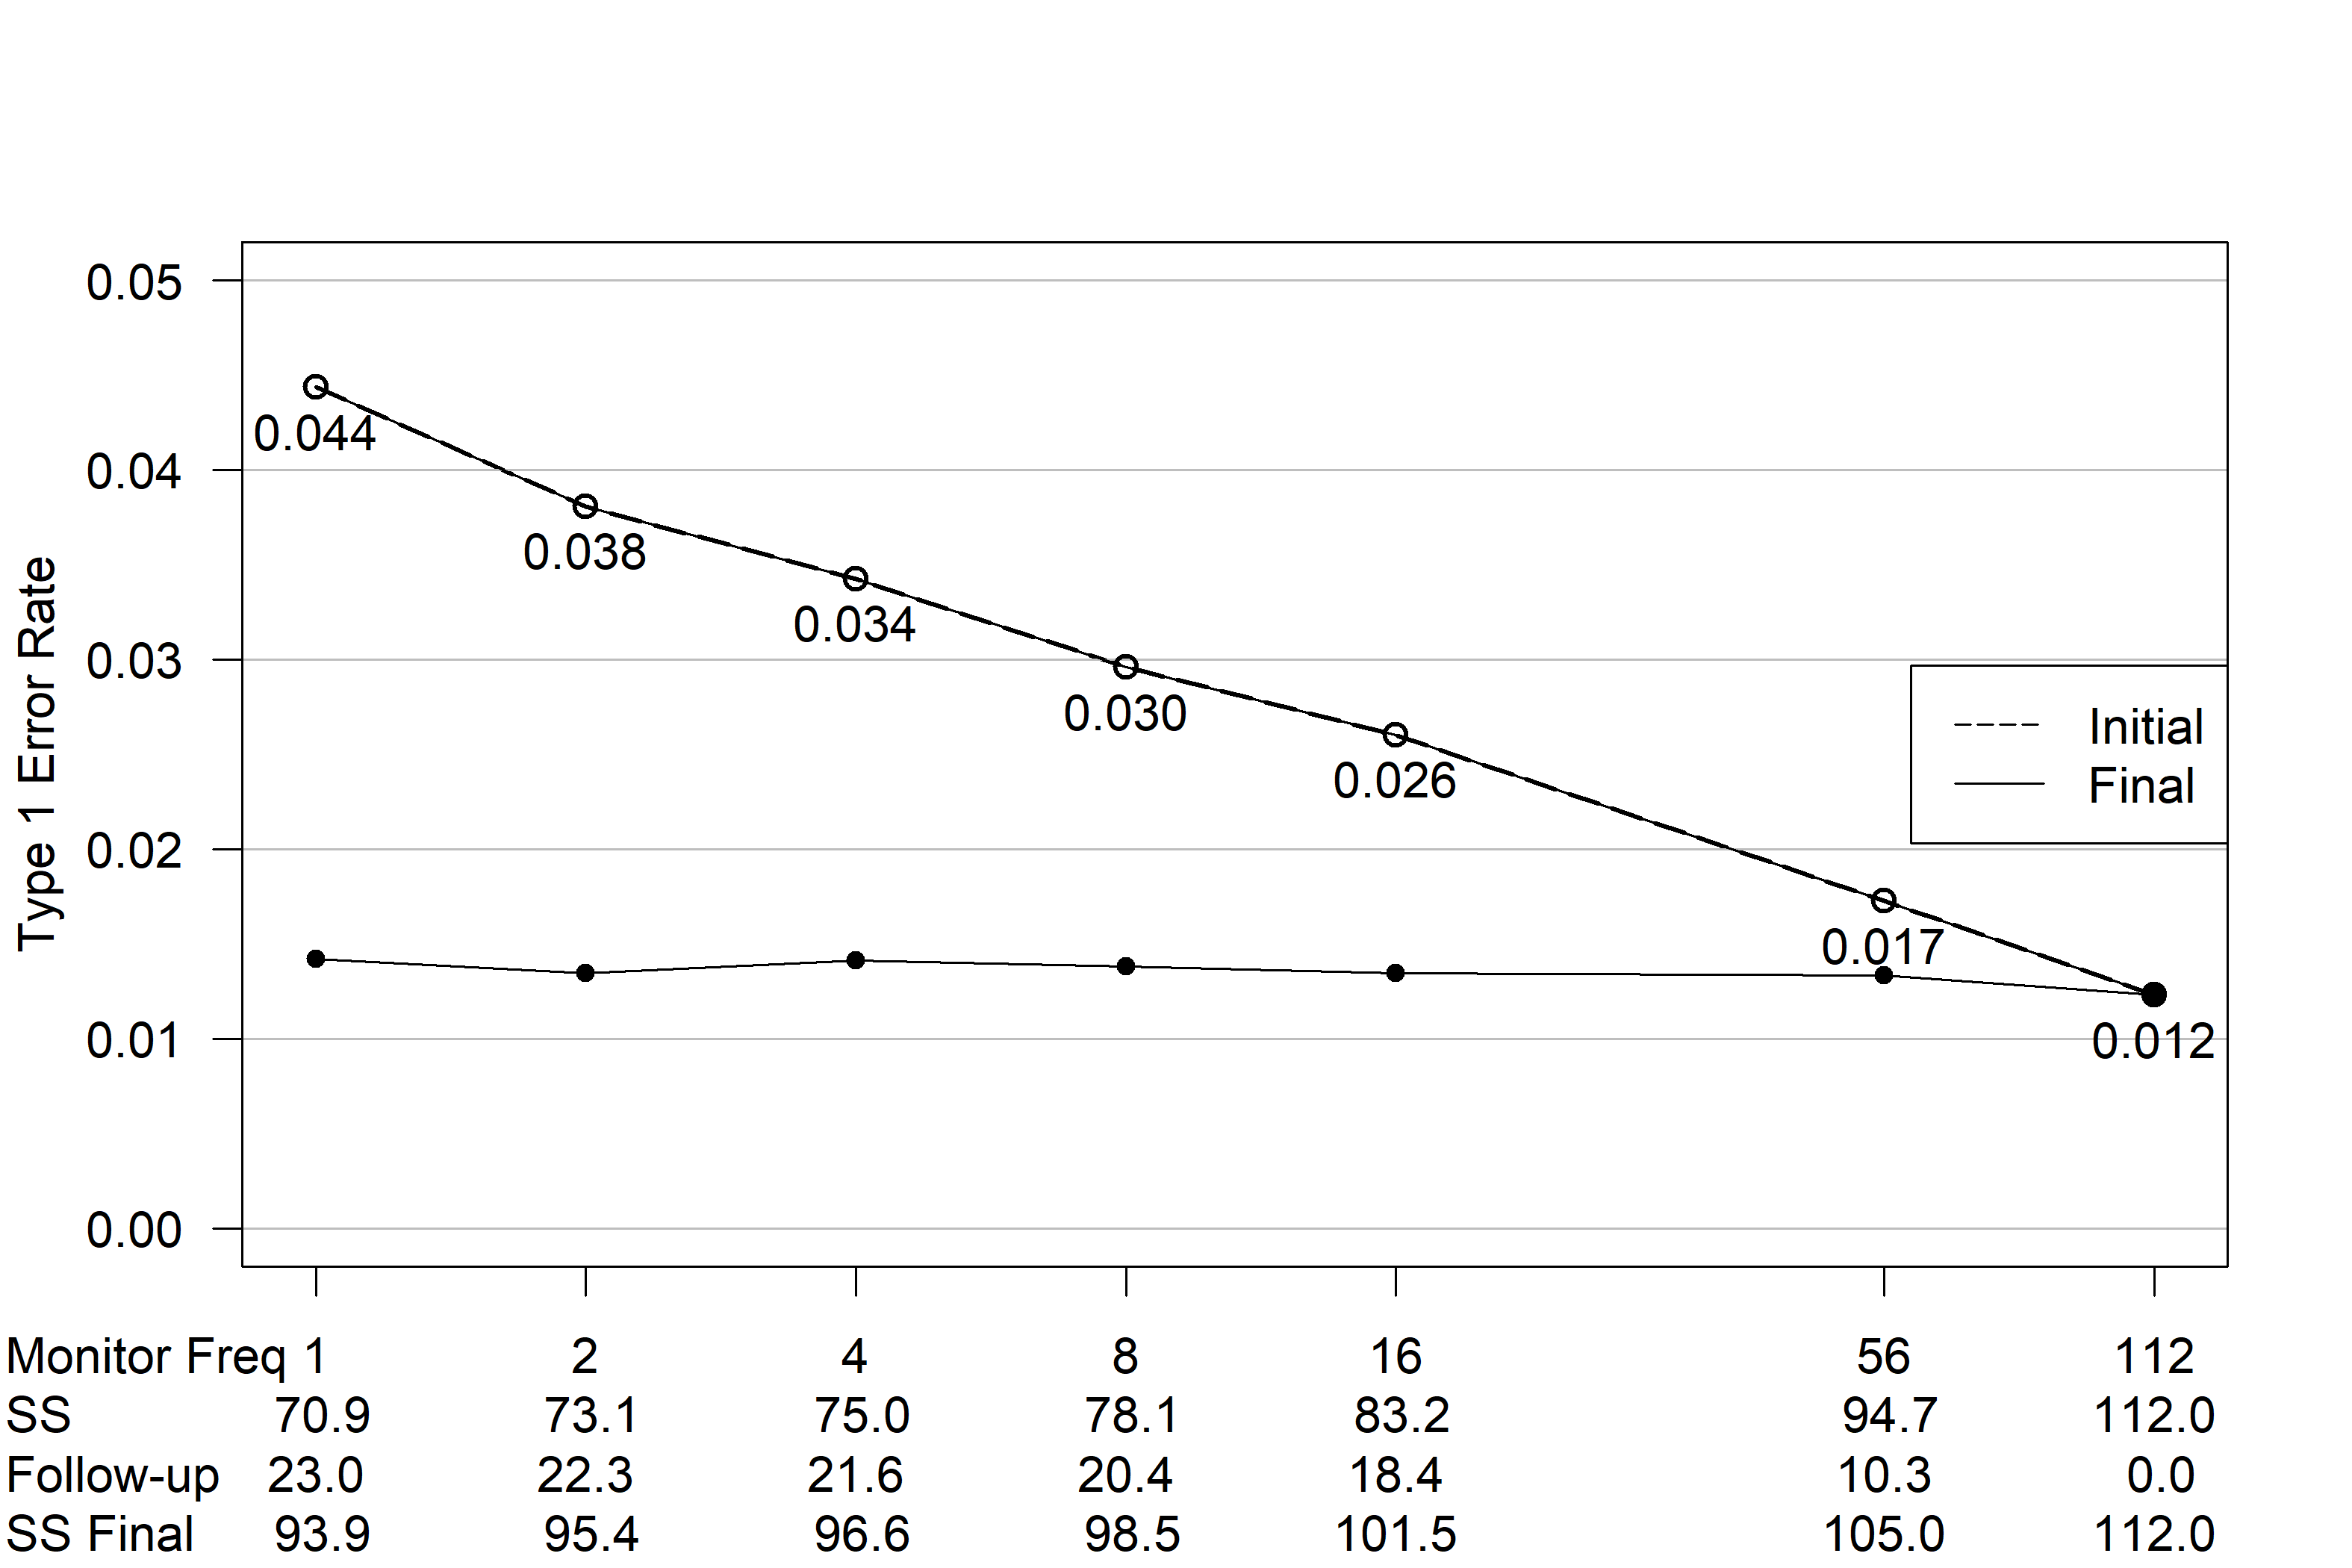
\includegraphics[width=6in]{figureS1.png}
%    \caption{Caption text 2}
%  \end{subfigure}
 
\end{center}
\end{figure}
%\item The two sides of the discussion: first is what happens during the trial regarding sequential monitoring, such as \% of time stopping early vs. trial done to completion and expected sample size. Second is the final determination of efficacy or futility and how that relates to Type 1 Error and power. 
%\item  Remember the best case for sequential monitoring is slow enrollment relative to outcome ascertainment. Slow enrollment means there is a benefit to ending trial early and reach a conclusion faster. Outcome ascertainment needs to be somewhat fast to ensure a good \# of outcomes are generated.

\subsection{Parallel Two-Group Design with Binary Endpoint}\label{sec:example2}
\subsubsection{Motivating Example}\label{sec:example2motivating}
We consider the trial ``The Pediatric Lupus Trial of Belimumab Plus Background Standard Therapy (PLUTO)" (NCT01649765) which was conducted between September 2012 and January 2018 \citep{Brunner2020}.
%
The study population was comprised of patients ages 5 though 17 with active systemic lupus erythematosus (SLE), defined as a baseline SELENA SLEDAI score of 6 or above on a scale of 0-105, where higher scores indicate more severe disease activity.
%
Patients were randomized to monthly dosing of either belimumab 10mg/kg or placebo, while continuing to receive standard of care therapy regardless of assignment.
%
The primary endpoint was a dichotomous variable reflecting a 4-point or greater reduction in SELENA SLEDAI score from baseline to week 52. 
%
The original study design included enrollment of 100 patients, the first 24 patients randomized in a 5:1 allocation ratio (belimumab:placebo) and the remaining 76 patients in a 1:1 ratio, resulting in 58 patients randomized to belimumab and 42 to placebo. 
%
The sample size was based on feasibility constraints rather than power considerations.
%
Data from two studies of belimumab in adults having the same disease resulted in a placebo response probability of $0.39$, and a 10mg/kg response probability of $0.51$. 
%
Using these values for the null and hypothesized response probabilities for the treatment group and assuming a response probability of 0.39 for the control group, a frequentist two-sided hypothesis test with confidence level $95\%$ and $80\%$ power would require 266 patients per group.
%
Ultimately, 93 patients were enrolled over approximately 52.5 months (approximately 1 patient enrolled per 17 days).
%
Clinical response was observed in 28 of 53 (52.8\%) of patients randomized to belimumab and in 17 of 40 (43.6\%) of patients randomized to placebo.

\subsubsection{Model Formulation \& Prior Elicitation}\label{sec:example2model}
We use this trial as a template to demonstrate our framework, in particular the performance response-adaptive sequential monitoring from Section \ref{sec:incorporating}. Response-adaptive sequential monitoring is necessary since the power analysis in Section \ref{sec:example2motivating} shows the need for many more patients than were available, therefore, a strategy for prospective incorporation of prior information must be implemented for the trial to have a chance of providing a compelling demonstration of efficacy through a pre-specified design.
%
The data $\bmath{D}$ are assumed to be independent Bernoulli random variables with response probability $\eta_0$ for the placebo group and $\eta_1$ for the treatment group, with $\theta=\eta_1-\eta_0$ denoting the difference in response probabilities. 
%
This trial has a superiority hypothesis of treatment to control with null difference in response probabilities, denoted by $\theta_0=0$.
%
An estimate for the pediatric response probability is denoted by $\eta_0=0.39$ (i.e. the sample proportion of responders from the pooled adult studies), and for purposes of monitoring, a plausible, clinically meaningful difference in response probabilities is $\theta_1=0.12$ (i.e. based on the pooled adult study's treatment response probability of $0.51$).% \citep{Furie2011,Navarra2011}.
%


The skeptical monitoring prior is $\pi_S(\theta,\eta_0)=\pi_S(\theta)\times\pi(\eta_0|\theta)$, where $\pi_S(\theta)$ is a concentrated skeptical prior.
%
The enthusiastic monitoring prior is $\pi_E(\theta,\eta_0)=\pi_E(\theta)\times\pi(\eta_0|\theta)$, where $\pi_E(\theta)$ is a default enthusiastic prior.
%
The probability of concluding efficacy at an interim analysis is made using a mixture prior with dynamic weight of the form \eqref{eq:adaptive_prior} as described in Section \ref{sec:incorporating}.
%
A 3-part mixture inference prior of the form \eqref{eq:3partmix} as described in Section \ref{sec:inferencepriors} was used to estimate the posterior mean and coverage probabilities for $\theta$.
%
%The locally non-informative prior is $\pi_{NI}(\theta,\eta_0)=\pi_{NI}(\theta)\times\pi(\eta_0|\theta)$.
%
%For the skeptical, enthusiastic, and locally non-informative priors, $\pi(\eta_0|\theta)$ is a flattened prior with mode value $0.39$ and tail probability condition $P(\eta_0>0.59 | \theta)=0.025$.

%, where $\pi_S(\theta)\sim\mathcal{GN}_{p=0.975,\Theta=[-1,1]}(\tilde{\mu}=\theta_0,q=\theta_1,\gamma=0.75)$. The value $\gamma=0.75$ reflects a concentrated distribution which was chosen to reflect a conservative opinion for added Type 1 error control. The enthusiastic monitoring prior is $\pi_E(\theta,\eta_0)=\pi_E(\theta)\times\pi(\eta_0|\theta)$, where $\pi_E(\theta)\sim\mathcal{GN}_{p=0.025,\Theta=[-1,1]}(\tilde{\mu}=\theta_1,q=\theta_0,\gamma=1)$. The value $\gamma=1$ was chosen as the default value. For both the skeptical and enthusiastic monitoring prior,$\pi(\eta_0|\theta)\sim\mathcal{GN}_{p=0.975,H=[max(-\theta,0),min(1,1+\theta)]}(\tilde{\mu}=0.39,q=0.59,\gamma=1.5)$. The value $\gamma=1.5$ was chosen to reflect a liberal opinion about the distribution of $\eta_0$. In general, it is recommended to use flattened priors for nuisance parameters.

A maximum sample size of $n_{\text{max}}=100$ was chosen based on the original trial protocol.
%
A minimum sample size of $n_{min}=70$ was chosen to provide an adequate number of placebo controls to be enrolled given the initial 5:1 allocation to the treatment group.
%
An interim analysis is completed after every two patients have outcomes beginning at $n_{min}$.

\subsubsection{Preposterior Analysis of Operating Characteristics}\label{sec:ex2operatingcharacteristics} 
The operating characteristics presented in this section are estimated using 20,000 simulated trials per value of $\theta$ using the trial design as described in Section \ref{sec:example2model}. The generating response probability in the placebo group was assumed to be 0.39, and the generating response probability in the treatment group was determined based on risk differences $\theta$ in $\{0, 0.06, 0.12, 0.18, 0.24\}$.

Panel A of Figure \ref{fig:ex2varyomega} shows the operating characteristics of this design using the adaptive weight monitoring prior and the 3-part mixture inference prior (see Web Appendix E for discussion of the mixture inference prior weights). 
%
When $\theta=0$, there is probability 0.008 of concluding efficacy at an interim analysis.
%
This probability increases to $0.193$ at $\theta_1=0.12$. While this does not attain traditional power thresholds, it is much greater than the respective probability of 0.006 using the default (non-adaptive) skeptical prior at this effect size.
%
At the effect size $0.24$ the probability of concluding efficacy increases to $0.711$, and the expected final sample size is 90.3 patients.

Panel B of Figure \ref{fig:ex2varyomega} shows the probability of stopping early for efficacy using a fixed weight mixture prior of the form \eqref{eq:inference_prior}  for efficacy monitoring with a fixed choice of $\omega$ chosen at the outset to be in the set $\{0.25,0.5,0.75,1\}$, and the associated sample sizes.
%
%Note that $\omega=1$ corresponds to the traditional skeptical prior, $\omega=0.5$ gives equal weight to the skeptical and enthusiastic components, and $\omega=0.25$ most of the weight is applied to the enthusiastic component.
%
The design based on the adaptive weight mixture behaves similar to the design based on the fixed weight prior that equally weighs the skeptical and enthusiastic prior.

\begin{figure}\begin{center}
      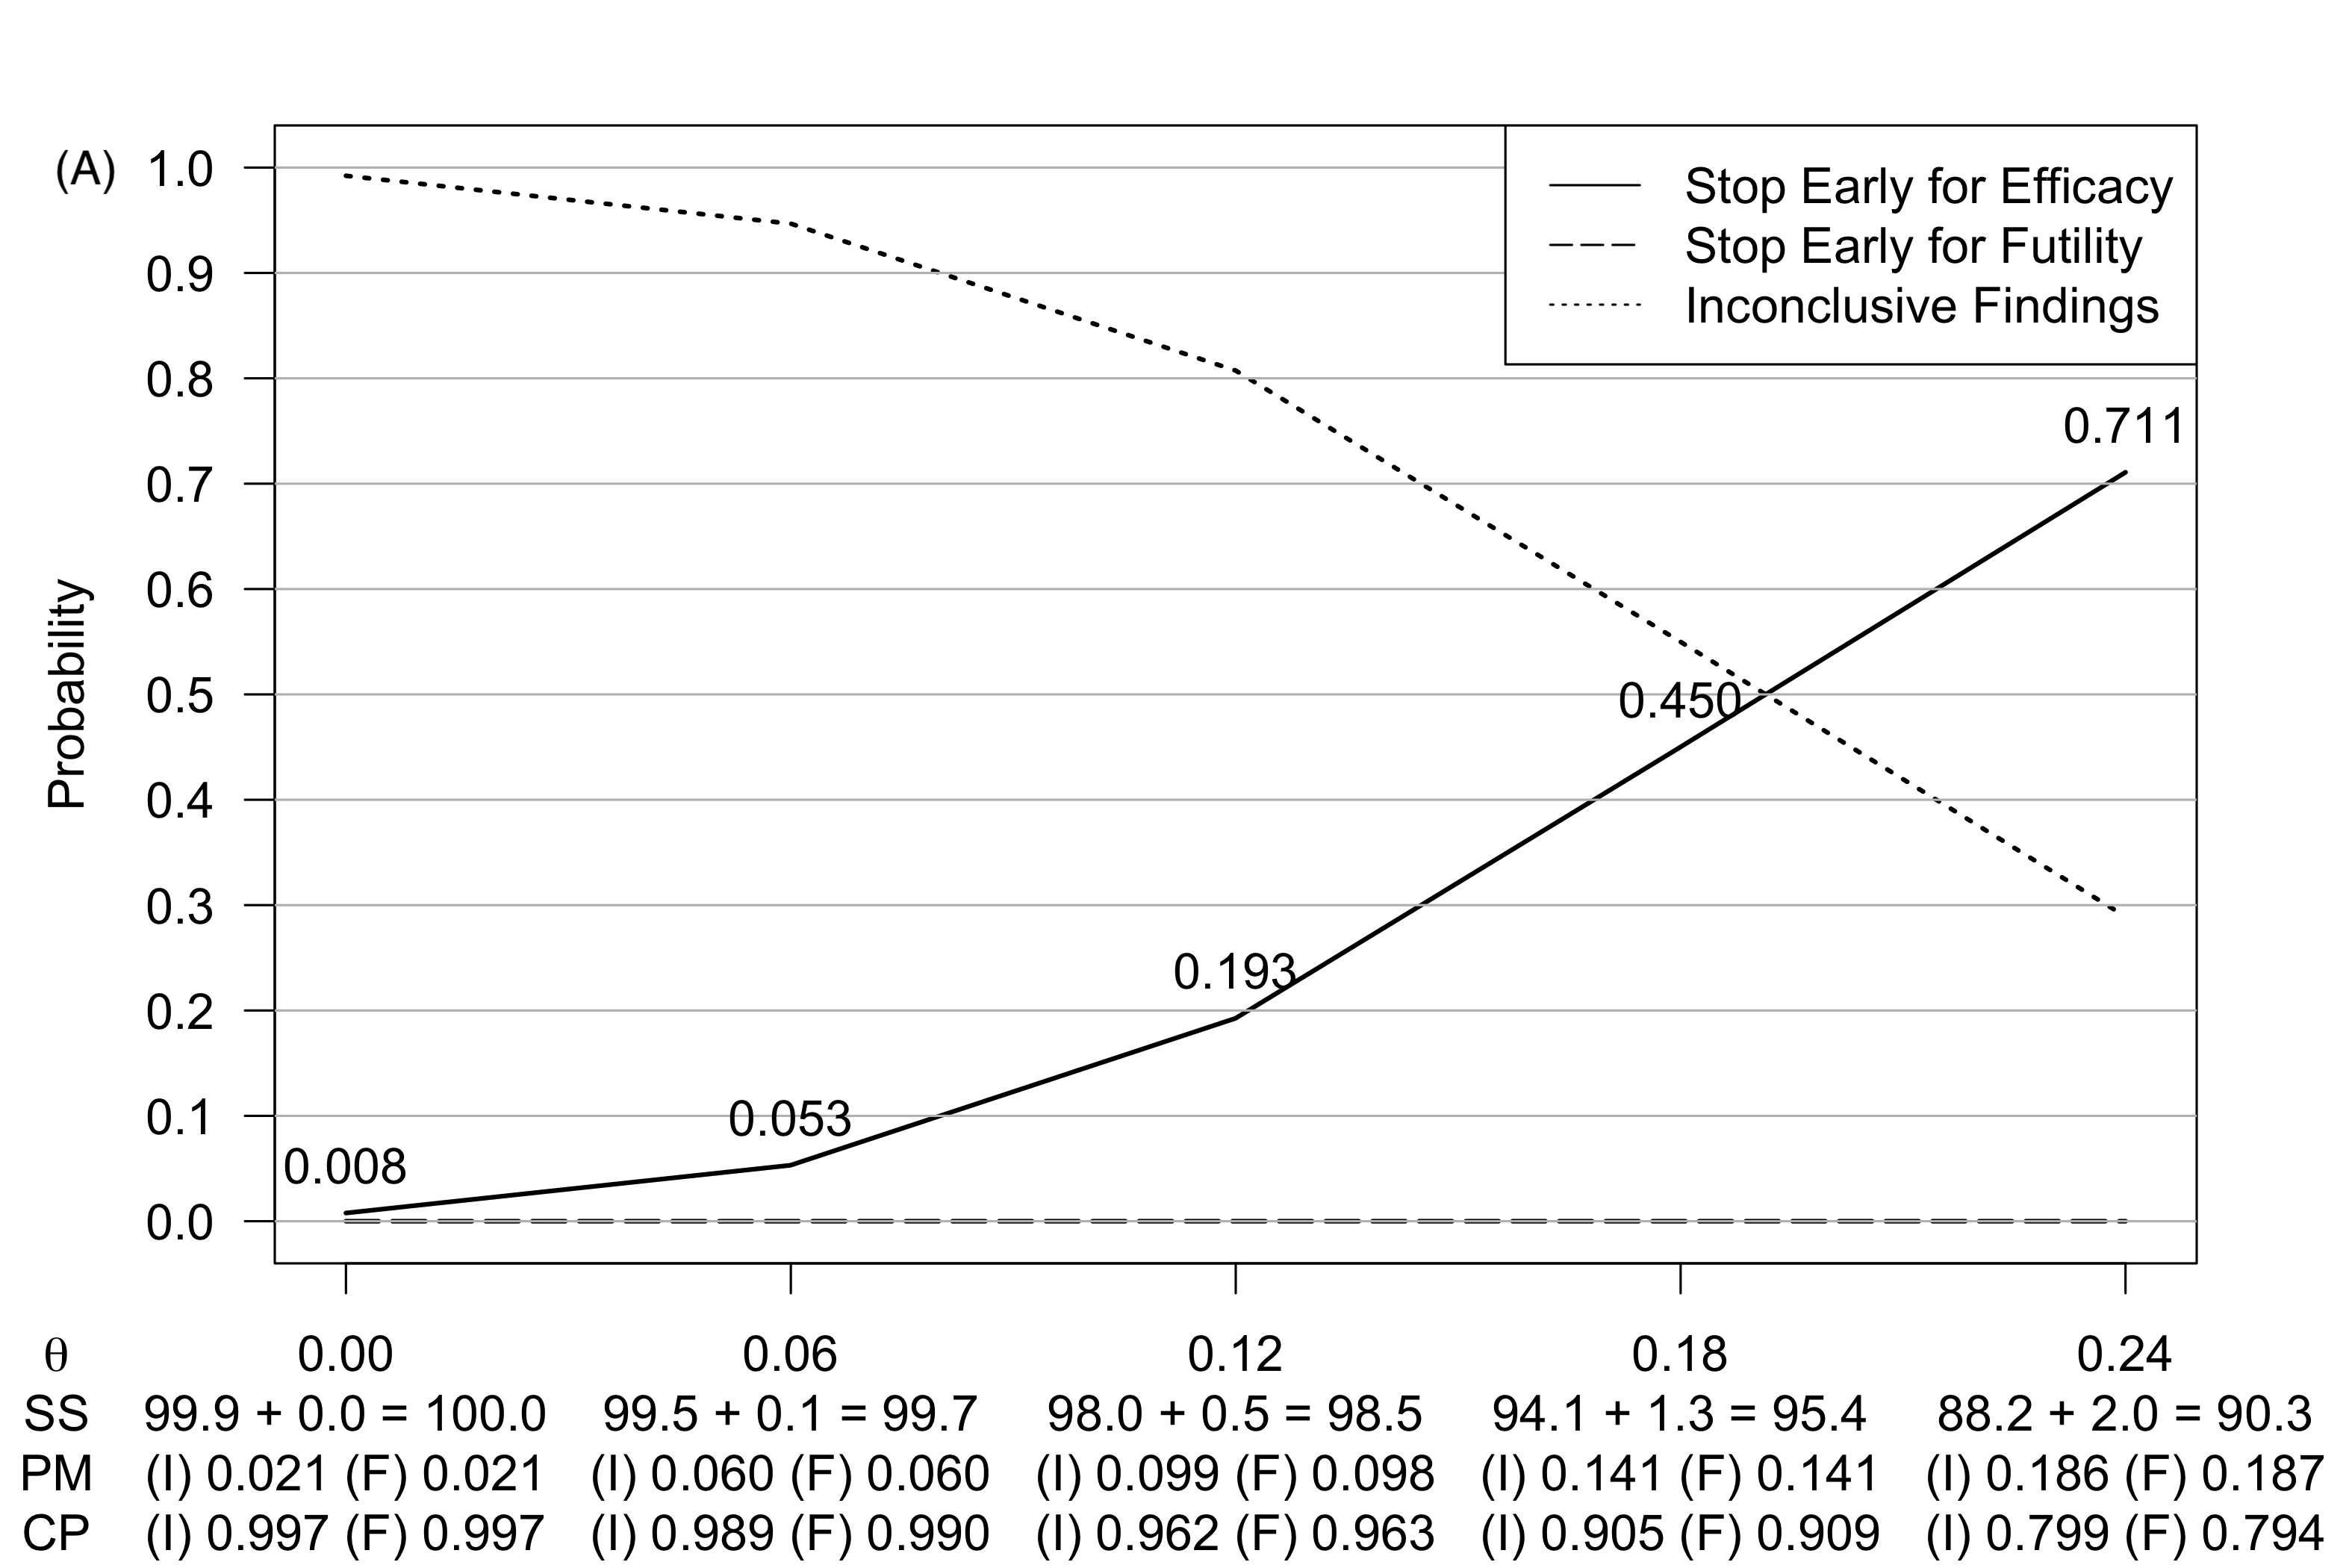
\includegraphics[width=6in]{figure9.png}
   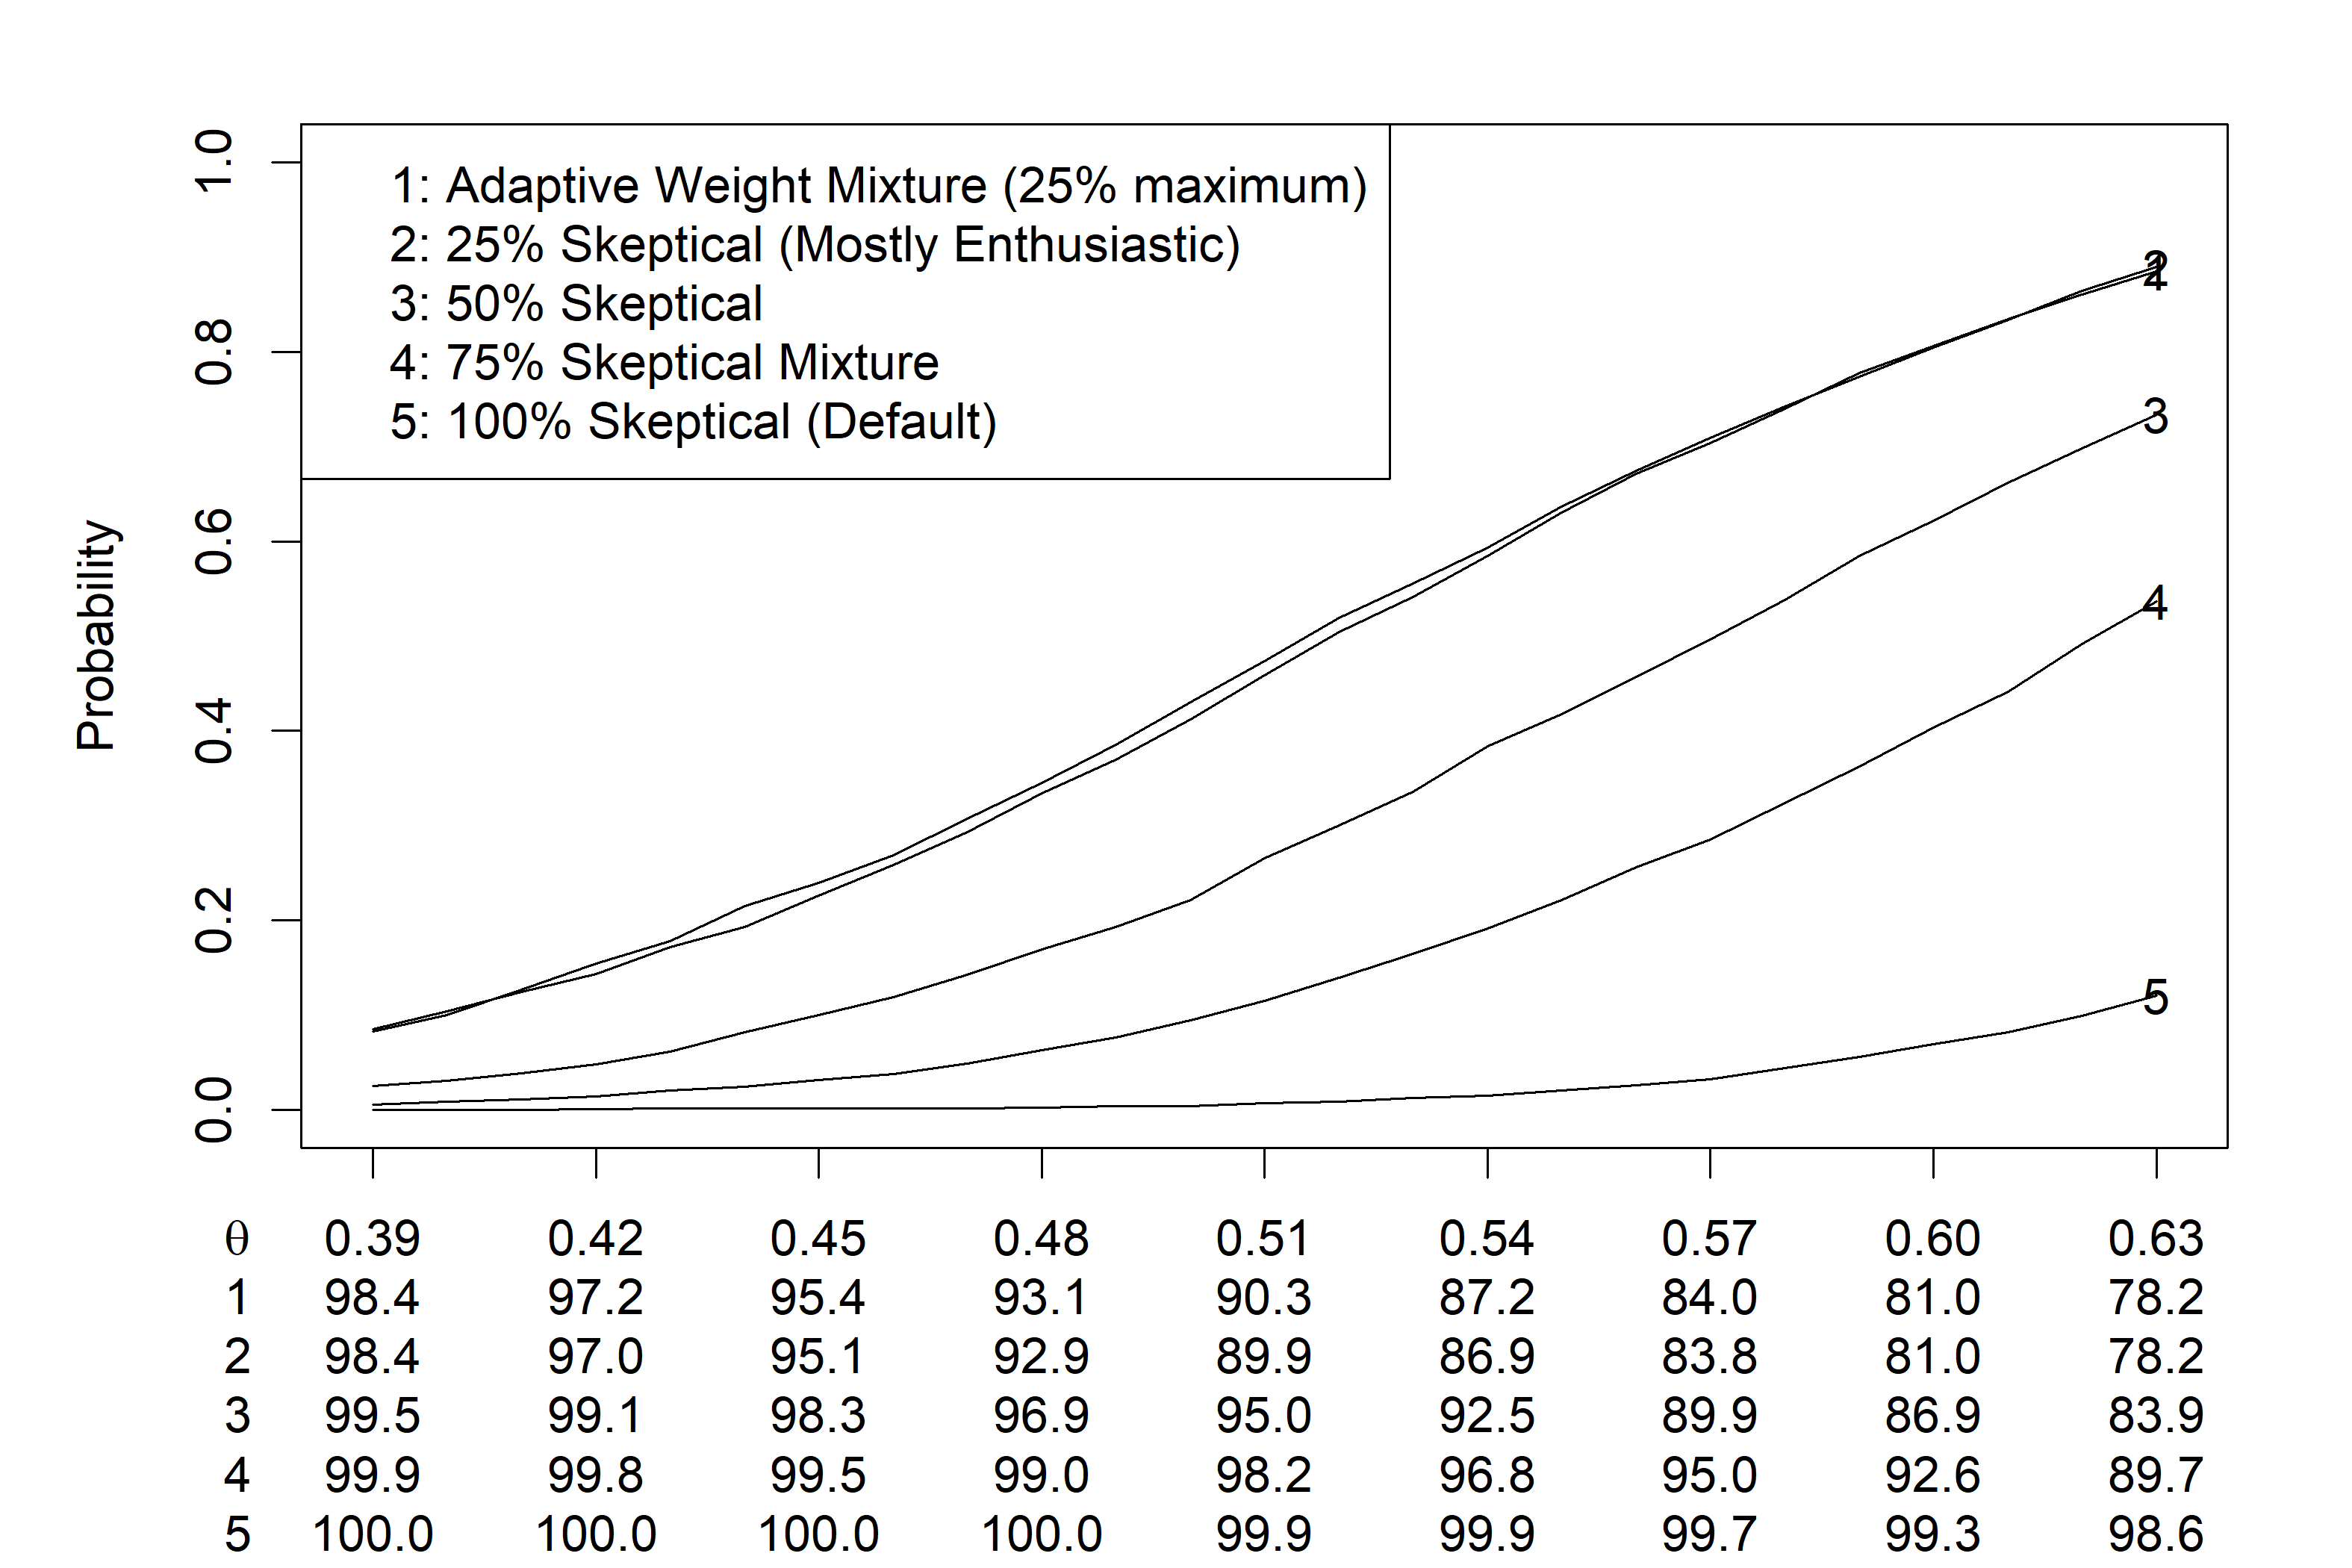
\includegraphics[width=6in]{figure6.png}
    \caption{A, Sequential design properties using adaptive weight monitoring prior (SS; mean sample size, PM; posterior mean, CP; coverage probability, (I); interim analysis, (F); final analysis). B, Probability of stopping for efficacy and associated sample sizes by true IP response probability $\theta$ with different choices of efficacy monitoring prior.}
\label{fig:ex2varyomega}
 \end{center}
\end{figure}

\section{Discussion}
In this paper, we present a structured framework for specifying monitoring priors and stoppage criteria for a Bayesian sequentially monitored clinical trial that is based on intuitive justification for the design quantities rather than being motivated by having pre-specified frequentist operating characteristics.
%
%To develop this methodology, we present a precise definition of sufficient level of evidence as it relates to the trial hypotheses and relevant external data, and use the generalized normal distribution for the monitoring priors.
%
%The inputs necessary to parameterize the monitoring priors and define the stoppage criteria are the sufficient level of evidence, the boundary null value for the treatment effect, and a plausible, clinically meaningful value for the treatment effect.
%
%This framework provides a reproducible process that emphasizes interpretability of the trial results as it directly relates to the design choices.
%
%We begin the presentation with fixed choices for the skeptical and monitoring priors, and then extend to adaptive mixtures based on assessments of prior-data conflict.
%
Consequently, the choice of monitoring prior and stoppage criteria are the same regardless of the frequency of data monitoring and the number of patients in progress at enrollment termination, although these factors do impact the operating characteristics of the trial.
%
Even though frequentist operating characteristics are not an explicit focus of the design, we demonstrate that the Bayesian approaches proposed provide good operating characteristics across a wide range of data monitoring frequencies and enrollment patterns.

Our results in Section \ref{sec:example2} can be compared to a post-hoc Bayesian hierarchical analysis which used data from two studies of the use of belimumab in adults \citep{Brunner2020}. Patients in the pediatric trial had 1.5 times the odds of clinical response with 95\% CI (0.6, 3.5), and a meta-analysis of the two adult studies showed an odds ratio of 1.6 with 95\% CI (1.3, 2.1). The analysis used a mixture prior which was a weighted sum of a skeptical prior centered at null effect with effective sample size equal to two pediatric patients and an informative prior resulting from the meta-analysis. When the weight of the informative component was 0.55 and above, efficacy was concluded based on a 95\% credible interval excluding one. The 0.55 weight of the informative component, interpreted as a 55\% weight on the relevance of the adult information to the pediatric population, was determined to be reasonable by the clinical team. Our method contrasts such a post-hoc analysis with the prospective use of a monitoring prior for efficacy which gives weight to the adult data at interim analyses, although both methods show the necessity of information borrowing. Our analyses show that for such a trial to have any chance of early stopping, it is necessary to borrow information for the skeptical monitoring prior as frequent data monitoring with a default skeptical prior has limited potential to conclude efficacy (see Figure \ref{fig:ex2varyomega}). In fact, the adaptive weight skeptical prior used in this example may be too conservative for this setting, and adaptive methods that include more liberal information borrowing could be used.

Although the examples provided are based on superiority trials with binary endpoints and response probabilities as the parameter of interest, the framework applies to any type of data and parameter of interest.
%
Future work will involve demonstrating the framework in Bayesian clinical trials with survival outcomes, such as large cardiovascular outcomes trials where frequent analysis of data may be useful to reduce excessive sample size requirements..


%\begin{table}
%\caption{This is a simple table.}
%\label{t:one}
%\begin{center}
%\begin{tabular}{lrrr}
%\Hline
%Estimator & \multicolumn{1}{c}{$\beta_1$} &  \multicolumn{1}{c}{$\beta_2$} & 
%\multicolumn{1}{c}{$\beta_3$} \\ \hline
%MLE & 10.18 & $-$3.26 & 0.13 \\
%OLS & 9.92 & $-$3.19 & 0.11 \\
%WLS & 9.88 & $-$3.33 & 0.12 \\
%\hline
%\end{tabular}
%\end{center}
%\end{table}

%  The \backmatter command formats the subsequent headings so that they
%  are in the journal style.  Please keep this command in your document
%  in this position, right after the final section of the main part of 
%  the paper and right before the Acknowledgements, Supporting Information (Supplementary %  Materials),   and References sections. 

\backmatter

%  This section is optional.  Here is where you will want to cite
%  grants, people who helped with the paper, etc.  But keep it short!

%\section*{Acknowledgements}

\vspace*{-8pt}



%  Here, we create the bibliographic entries manually, following the
%  journal style.  If you use this method or use natbib, PLEASE PAY
%  CAREFUL ATTENTION TO THE BIBLIOGRAPHIC STYLE IN A RECENT ISSUE OF
%  THE JOURNAL AND FOLLOW IT!  Failure to follow stylistic conventions
%  just lengthens the time spend copyediting your paper and hence its
%  position in the publication queue should it be accepted.

%  We greatly prefer that you incorporate the references for your
%  article into the body of the article as we have done here 
%  (you can use natbib or not as you choose) than use BiBTeX,
%  so that your article is self-contained in one file.
%  If you do use BiBTeX, please use the .bst file that comes with 
%  the distribution.  In this case, replace the thebibliography
%  environment below by 
%
\bibliographystyle{biom} 
\bibliography{jan-07-bib}

%\begin{thebibliography}{}
%
%\bibitem{ } Cox, D. R. (1972). Regression models and life tables (with
%discussion).  \textit{Journal of the Royal Statistical Society, Series B}
%\textbf{34,} 187--200.
%
%\bibitem{ }  Hastie, T., Tibshirani, R., and Friedman, J. (2001). \textit{The 
%Elements of Statistical Learning: Data Mining, Inference, and Prediction}.
%New York: Springer.
%
%\end{thebibliography}

%  If your paper refers to supporting web material, then you MUST
%  include this section!!  See Instructions for Authors at the journal
%  website http://www.biometrics.tibs.org

%\vspace*{-8pt}

%\vspace{-0.40in}
%\vspace{0.01in}
\section*{Supporting Information}
Web Appendices referenced in Sections 2 and 3 are available with this paper at the Biometrics website on Wiley Online Library. A GitHub repository contains the programs and other resources needed to reproduce the analyses presented in this paper 

\noindent (https://github.com/psioda/Bayesian-Sequential-Monitoring). The software provided was written using R \citep{R2017} version 4.0.0.



%\appendix

%  To get the journal style of heading for an appendix, mimic the following.

%\section{}
%\subsection{Title of appendix}

%% latex table generated in R 4.0.0 by xtable 1.8-4 package
% Tue Jul 14 12:05:34 2020
\begin{table}[ht]
\centering
\begin{tabular}{llrrrr}
  \hline
  \hline
0.4 & FUT INITIAL & 0.7572 & 0.7653 & 0.8069 & 0.8183 \\ 
   & FUT FINAL & 0.5862 & 0.5930 & 0.6371 & 0.6455 \\ 
   & SS & 71.0198 & 73.0444 & 66.6849 & 68.6982 \\ 
  0.535 & FUT INITIAL & 0.0260 & 0.0251 & 0.0384 & 0.0370 \\ 
   & FUT FINAL & 0.0137 & 0.0127 & 0.0199 & 0.0193 \\ 
   & SS & 56.8978 & 66.8005 & 56.1953 & 66.4028 \\ 
  0.67 & FUT INITIAL & 0.0000 & 0.0000 & 0.0000 & 0.0000 \\ 
   & FUT FINAL & 0.0000 & 0.0000 & 0.0000 & 0.0000 \\ 
   & SS & 22.9456 & 27.8308 & 23.0299 & 27.8094 \\ 
   \hline
\end{tabular}
\end{table}


\label{lastpage}

\end{document}